\PassOptionsToPackage{full}{textcomp}
% include symmetric to place margins left and right instead of right only
% nohyper, nobib?
\documentclass[nobib,a4paper,twoside,notoc,justified,marginals=justified]{tufte-book}
% \documentclass{caesar_book}
\usepackage[utf8]{inputenc}

% \usepackage{hyperref}
\hypersetup{colorlinks}

% \usepackage{setspace}
% \newcommand{\newthought}[1]{\textsc{#1}}

%%
% For nicely typeset tabular material
\usepackage{booktabs}

% fix too many alphabets error
\usepackage{amsmath, amssymb}
\newcommand\hmmax{0}
\newcommand\bmmax{0}

% fix margins?
% \usepackage{marginfix}

\usepackage{enumitem, bm, xcolor, braket, dsfont, graphicx, cancel}
\usepackage[multidot]{grffile}
% \usepackage[colorlinks, linkcolor = red, citecolor = black, filecolor = black, urlcolor = blue]{hyperref} 
% \usepackage{nameref}
% \hypersetup{colorlinks}
\usepackage{algorithmic}
\usepackage{todonotes}

% Quotes
\usepackage{epigraph}
\setlength\epigraphwidth{10cm}
\setlength\epigraphrule{0pt}

%% style
% \usepackage{mathptmx}
% \usepackage{setspace}
% \linespread{1.0}

% \iflarger
%\AtBeginDocument{%
%	\fontsize{12}{14}\selectfont
%}%
% \else\fi


% integrate amsthm and txmath
\usepackage{savesym}
\usepackage{amsthm}
\savesymbol{openbox}
\usepackage{newtxtext,newtxmath}
\restoresymbol{TX}{openbox}

% theorems
\newtheorem*{theorem}{Theorem}
\newtheorem*{thm}{Theorem}

% shorthand
\renewcommand{\t}[1]{\text{#1}}
\renewcommand{\d}{{\rm d}}
\renewcommand{\b}[1]{{\bf #1}}
\newcommand{\B}[1]{\mathbf{#1}}
\newcommand{\D}[1]{{#1}^\dagger}
\newcommand{\fD}[1]{{#1}^{ \phantom{\dagger}}}
\renewcommand{\P}[1]{{#1}^\prime}
\newcommand{\fP}[1]{{#1}^{\phantom{\prime}}}
\newcommand{\im}{{\rm i}}
\newcommand{\halb}{\frac{1}{2}}
\DeclareMathOperator{\Tr}{Tr}
\newcommand{\kb}{k_{\rm B}}
\newcommand{\sigmaA}{\sigma^\mathrm{A}}
\newcommand{\sigmaAOS}{\sigma^\mathrm{A}_\mathrm{OS}}
\newcommand{\sigmaAMD}{\sigma^\mathrm{A}_\mathrm{MD}}

% transpose
\usepackage{relsize}
\newcommand{\tp}[1]{{#1}^{\mathrm t}}
% \!\: = 1mu distance; \!\; = 2mu (\, = 3mu)
\newcommand{\itp}[1]{{#1}^{\!\:\scalebox{0.55}[1.0]{\( - \)}1 \mathrm t}}

% comments:
% dblue: https://coolors.co/1f77b4
\definecolor{dblue}{RGB}{31,119,180}
\definecolor{dblue_light}{HTML}{5AAAE3}
\definecolor{purple_light}{HTML}{A61EB3}
\definecolor{yellow1}{HTML}{E7EB90}
\definecolor{yellow2}{HTML}{FADF63}
\definecolor{yellow3}{HTML}{E6AF2E}
\definecolor{red_light}{HTML}{FE404A}
\definecolor{cite}{HTML}{2BB31E}
\definecolor{djordje}{RGB}{192,225,215}
\newcommand{\MOVE} [1] 
{\todo[inline,backgroundcolor=red_light, bordercolor=white]{{\bf MOVE:} #1}}
\newcommand{\REM} [1] 
{\todo[inline,backgroundcolor=dblue_light, bordercolor=white]{{\bf REM:} #1}}
\newcommand{\CITE} [1] 
{\todo[inline,backgroundcolor=cite, bordercolor=white]{{\bf CITE:} #1}}
% \newcommand{\FK}[1]{\textcolor{blue}{{\bf #1 }}}
\newcommand{\TODO} [1] 
{\todo[inline,backgroundcolor=red, bordercolor=white]{{\bf TODO:} #1}}
\newcommand{\ADD} [1] 
{\todo[inline,backgroundcolor=red, bordercolor=white]{{\bf ADD} #1}}
\newcommand{\FK} [1] 
{\todo[inline,backgroundcolor=yellow2, bordercolor=white]{{\bf Florian:} #1}}
\newcommand{\idea} [1] 
{\todo[inline,backgroundcolor=red, bordercolor=white]{{\bf idea:} #1}}
\newcommand{\inlinecomment}[1]{\textcolor{red}{{\bf #1 }}}
\newcommand{\prelim}[1]{\textcolor{red}{{\bf prelim:} {\it #1 }}}
\newcommand{\CC} [1] 
{\todo[inline,backgroundcolor=yellow3, bordercolor=white]{{\bf CC:} #1}}

% Tufte

% TOC
% https://tex.stackexchange.com/questions/121790/how-to-generate-a-full-width-table-of-contents-tufte-book
\usepackage{lipsum,mdframed}
\definecolor{secnum}{RGB}{13,151,225}
\definecolor{ptcbackground}{RGB}{212,237,252}
\definecolor{ptctitle}{RGB}{0,177,235}

\setcounter{secnumdepth}{3}

\usepackage[toc]{appendix}
% \usepackage{titletoc}
% \usepackage{etoolbox}
\setcounter{tocdepth}{1}
%\pretocmd{\tableofcontents}{\begin{mdframed}\let\cleardoublepage\relax}{}{}
%  \apptocmd{\tableofcontents}{\end{mdframed}}{}{}

% The fancyvrb package lets us customize the formatting of verbatim
% environments.  We use a slightly smaller font.
\usepackage{fancyvrb}
\fvset{fontsize=\normalsize}

%%
% Prints argument within hanging parentheses (i.e., parentheses that take
% up no horizontal space).  Useful in tabular environments.
\newcommand{\hangp}[1]{\makebox[0pt][r]{(}#1\makebox[0pt][l]{)}}

%%
% Prints an asterisk that takes up no horizontal space.
% Useful in tabular environments.
\newcommand{\hangstar}{\makebox[0pt][l]{*}}

%%
% Prints a trailing space in a smart way.
\usepackage{xspace}

% Prints the month name (e.g., January) and the year (e.g., 2008)
\newcommand{\monthyear}{%
  \ifcase\month\or January\or February\or March\or April\or May\or June\or
  July\or August\or September\or October\or November\or
  December\fi\space\number\year
}

% http://tex.stackexchange.com/a/140164/1913
% \ifxetex
% xetex fix https://tex.stackexchange.com/a/200725/91226
%\ifx\ifxetex\ifluatex\else % if lua- or xelatex   \newcommand{\textls}[2][5]{%
%    \begingroup\addfontfeatures{LetterSpace=#1}#2\endgroup
%  }
%  \renewcommand{\allcapsspacing}[1]{\textls[15]{#1}}
%  \renewcommand{\smallcapsspacing}[1]{\textls[10]{#1}}
%  \renewcommand{\allcaps}[1]{\textls[15]{\MakeTextUppercase{#1}}}
%  \renewcommand{\smallcaps}[1]{\smallcapsspacing{\scshape\MakeTextLowercase{#1}}}
%  \renewcommand{\textsc}[1]{\smallcapsspacing{\textsmallcaps{#1}}}
%\fi


% Prints an epigraph and speaker in sans serif, all-caps type.
\newcommand{\openepigraph}[2]{%
  %\sffamily\fontsize{14}{16}\selectfont
  \begin{fullwidth}
  \sffamily\large
  \begin{doublespace}
  \noindent\allcaps{#1}\\% epigraph
  \noindent\allcaps{#2}% author
  \end{doublespace}
  \end{fullwidth}
}

% Inserts a blank page
\newcommand{\blankpage}{\newpage\hbox{}\thispagestyle{empty}\newpage}

\usepackage{units}

% Typesets the font size, leading, and measure in the form of 10/12x26 pc.
\newcommand{\measure}[3]{#1/#2$\times$\unit[#3]{pc}}

% Macros for typesetting the documentation
\newcommand{\hlred}[1]{\textcolor{Maroon}{#1}}% prints in red
\newcommand{\hangleft}[1]{\makebox[0pt][r]{#1}}
\newcommand{\hairsp}{\hspace{1pt}}% hair space
\newcommand{\hquad}{\hskip0.5em\relax}% half quad space
\newcommand{\na}{\quad--}% used in tables for N/A cells

% Generates the index
\usepackage{makeidx}
\makeindex


\begin{document}

% Front matter
\frontmatter
\addtocontents{toc}{\protect\setcounter{tocdepth}{0}}
  
%  % r.1 blank page
%  \blankpage
%  
%% r.3 full title page
%\maketitle

% r.5 contents
\tableofcontents

% \listoffigures

% \listoftables

% r.7 dedication
%\cleardoublepage
%~\vfill
%\begin{doublespace}
%  \noindent\fontsize{12}{12}\selectfont\itshape
%  \nohyphenation
%  \hfill To my teachers.
%\end{doublespace}
%\vfill
%\vfill


% r.9 introduction
\cleardoublepage

\chapter{Introduction}
\epigraph{\singlespacing \it ``Die Zeit des unbedenklichen Wirtschaftens mit den Energiequellen und Stofflagern, die uns die Natur zur Verfügung gestellt hat, wird wahrscheinlich schon für unsere Kinder nur noch die Bedeutung einer vergangenen Wirtschaftsepoche haben.''}{W. Schottky, 1929~\cite{Schottky1929}}
% [ ] Why thermal conductivity?
% [ ] Why novel thermal insulators?
% [ ] Why computational materials science?
\newthought{One of the major challenges} humankind faces in the 21th century is the responsible and sustainable handling of the earth's natural resources.  Yet, most energy today is lost as waste heat during the transformation of raw energy sources to usable power. To date, there is no fuel based heat engine that exceeds an efficiency of 50\,\% and often it is even worse~\cite{eia}. 
Since gas- and aircraft-turbines are essentially Carnot engines, their efficiency and core power are directly related to combustion temperature~\cite{Clarke2012,Perepezko2009}. This relationship has been taken advantage off during the past 30 years by developing 
ceramics with high thermal resistivity that are nowadays applied as \emph{thermal barrier coatings} on turbine airfoils in heat engines: thin heat insulating layers that allow to operate a turbine at higher temperatures, thereby increasing its efficiency~\cite{Clarke2003}.

A complementary strategy is to recycle waste heat where it occurs. One way of achieving this is by using the \emph{thermoelectric effect} to  generate electric power from temperature gradients~\cite{Snyder2008}. The main obstacle preventing mass operation is the limited conversion rate (figure of merit) $zT$ of even the most advanced thermoelectric materials known to date. To make matters worse, these materials often contain heavy metals and are toxic, and their manufacturing process is difficult and expensive~\cite{Nolas2001}. Recent advancements in the field, such as the discovery of a high thermoelectric figure of merit in the lead-free material Tin Selenide~\cite{zhao2014}, offer hope that novel materials with significant figure of merit that are non-toxic, easy and cheap to produce, and consist of abundant elements, can be found.

\newthought{A key physical property} of both thermal barrier coatings (TBCs) and thermoelectrics is their thermal conductivity $\kappa$. In the case of thermoelectrics, the figure of merit is inversely proportional to $\kappa$~\cite{Nolas2001}:
\begin{align}
zT = \frac{S^2 \sigma_{\rm el}}{\kappa} T~,
\label{eq:zT}
\end{align} 
where $T$ dentoes the temperature, $S$ the Seebeck coefficient, and $\sigma_{\rm el}$ is the electrical conductivity.
A prerequisite to finding better thermoelectrics or TBCs is to find materials which are thermally insulating. These are typically non-metals, since the free electrons in metals are good heat carriers, and most of the known thermoelectrics are thermally insulating inorganic semiconductors~\cite[p.\,15]{Nolas2001}.

Despite the technological need, systematic knowledge of thermal conductivities in inorganic compounds is scarce. A database like Springer Materials only lists thermal conductivities for about 200~of these compounds~\cite{SpringerMaterials}, which is partially due to the fact that accurate measurements of thermal conductivity are challenging to perform and reproducibility between different experimental groups is often not guaranteed~\cite{wei2016}. As a consequence, thermal conductivity is not systematically understood beyond semi-empirical and phenomenological trends in a very limited number of simple material classes~\cite{morelli2006}.

\newthought{The aim of this work} is therefore to open a new pathway for overcoming the problem of limited data by devising a route to systematically scan material space for thermal insulators and calculate their thermal conductivities from first principles. 

While the theoretical foundations of thermal transport in non-metals are about one hundred years old,\footnote{The many pitfalls in early attempts to describe thermal transport in semiconductors was summarized by Peierls in his memorial text in honor of Wolfgang Pauli~\cite{Peierls1960}.} the simulation of thermal conductivities with predictive accuracy from first principles only emerged in the past fifteen years in the framework of Boltzmann transport theory~\cite{Broido2007}. Yet, as we will see later, thermal insulators are often strongly \emph{anharmonic} and require a non-perturbative treatment to describe their dynamical properties accurately. Such a fully non-perturbative treatment in terms of \emph{ab initio} Green-Kubo theory is available since five years~\cite{Marcolongo2016,Carbogno2016}. However, the number of solid materials computed by the latter approach is very small: Solid silicon and zirconia~\cite{Carbogno2016}, ice X~\cite{Grasselli2020}, and amorphous silica~\cite{Marcolongo2020}. 

\newthought{The approach adopted in this work is therefore twofold:} After reviewing the relevant theoretical tools necessary to simulate heat transport in thermal insulators, we describe how to assess anharmonicity in a quantitative and paremeter-free way. In a second step, we use this ``measure of anharmonicity'' to identify candidate thermal insulators. We subsequently compute non-perturbative thermal conductivities for 60 materials with nearly experimental accuracy, thereby increasing the number of materials studied with \emph{ab initio} Green Kubo by an order of magnitude while suggesting several new materials as effective thermal insulators. Furthermore, the data is used to test trends in material space previously based on experimental data, such as the quantitative relation between thermal conductivity and anharmonicity.


\section*{Organization of the Thesis}
The thesis is split into two parts: The first part introduces the theoretical concepts necessary to understand thermal transport in materials from an \emph{ab initio} perspective.
In chapter one, we will introduce the quantum-mechanical many-body problem and describe the necessary steps and key approximations that lead to Kohn-Sham density functional theory as a way of solving the electronic problem in practice. Chapter two will describe the key concepts of nuclear dynamics that are necessary to study thermodynamical properties of materials, such as heat transport: The chapter introduces the harmonic approximation as a powerful starting point for studying dynamical propertis of matter, and the fully non-perturbative treatment of nuclear dynamics and thermodynamic properties in terms of molecular dynamics simulations. Chapter three is dedicated to heat transport theory in the framework of linear response as formulated in the Green-Kubo formalism. The purpose is to clarify how heat transport emerges from the many-body Schr\"odinger equation, and how, in principle, thermal conductivity can be computed from first principles.

The second part can be understood as an application of this body of theory and is devoted to the investigation of materials in the context of heat transport. In chapter four, we introduce a novel concept to quantify the anharmonicity of material as a means to detect materials that should be treated non-perturbatively. As we will see, this quantitity directly correlates with a material's thermal conductivity and therefore enables to predict candidate thermal insulators. Chapter five is devoted to introducing the technical details necessary to run \emph{ab initio} Green Kubo (aiGK) simulations in practice. In chapter six, we present results for \CHECK 60~materials, first for \CHECK 20 where experimental reference is available to benchmark the aiGK method, then for the remaining materials where thermal conductivity was previously unknown. In this context, we dicsuss the underlying microscopic mechanisms, in particular the relation to anharmonicity.

After discussing our results, we conclude with a summary and an outlook on new questions that arose in the course of this work.


%%
% Start the main matter (normal chapters)
\mainmatter
\addtocontents{toc}{\protect\setcounter{tocdepth}{2}}  % later -> 1

\part{Theoretical Foundation}

\chapter{The Many Body Problem}
\input{./parts/1_dft.tex}

\chapter{Nuclear and Lattice Dynamics}
\label{chp:dynamics}
In the previous chapter, we have seen how the many-body problem can be decoupled into an electronic problem %given by Eq.\,\eqref{eq:Hsolution1}, 
which can be solved in the framework of DFT, and a nuclear problem %given by Eq.\,\eqref{eq:chi2} 
that describes the dynamical properties of the nuclei. This was achieved by means of the Born-Oppenheimer approximation where electron-nucleus interactions beyond a parametric dependence on each other are neglected~\cite{BornOppenheimer}.
\mscomment{dynamics are decoupled}

\newthought{We will now approach} the description of the nuclear dynamics from two sides: First, we introduce the \emph{harmonic approximation} in which the nuclear Schr\"odinger equation is solved for an approximated potential in terms of vibrational eigenmodes. We will discuss extended systems next, in particular crystalline systems with long-range order.
Second, we treat the nuclei as \emph{classical} particles on the full, non-truncated Born-Oppenheimer potential $E^{\rm BO} ({\bf R})$. This will lead to the formulation of \emph{ab initio molecular dynamics} (aiMD). In a last step, we will connect the two approaches to allow for extracting phonon properties from MD simulations.
As no electron will appear anymore, $N \equiv N_{\rm Nuc}$ will henceforth denote the number of nuclei in the system of interest, and we denote the Born-Oppenheimer potential simply as \emph{the} potential, $E^{\rm BO} ({\bf R}) \equiv \mathcal V ({\bf R})$.

\newthought{To set the stage, we recall the Schr\"odinger equation} for the nuclear wavefunction $\chi ({\bf R})$ corresponding to the electronic ground state as initially defined in Eq.\,\eqref{eq:chi2},
\begin{align}
\left( \mathcal T + \mathcal V ({\bf R}) - E \right) \chi ({\bf R})
= 0~,
\label{eq:BOSE}
\end{align}
where
\begin{align}
\mathcal  T
= \sum_I \frac{- \hbar^2}{2 M_I} \frac{\partial^2}{\partial {\bf R}_I^2}~,
\label{eq:Tnuc2}
\end{align}
is the nuclear kinetic-energy operator as before.

\newpage
\section{Harmonic Approximation}
\label{sec:HA}
The Born-Oppenheimer potential $\mathcal V ({\bf R})$ in Eq.\,\eqref{eq:BOSE} is an ordinary function of the\marginnote{Remember $N \equiv N_{\rm Nuc}$.} $3 N$ coordinates ${\bf R} = ({\bf R}_1, \ldots, {\bf R}_{N})$ and therefore can be expanded as a Taylor series in displacements ${\bf U} \equiv \Delta {\bf R}$ about a given configuration ${\bf R}^0$,~i.\,e.,
\begin{align}
\begin{split}
  \mathcal V ({\bf R} = {\bf R}^0 + {\bf U})
    = \mathcal V ({\bf R}^0)
    &+ \sum_{I, \alpha} 
      \left. \frac{\partial \mathcal V({\bf R})}{\partial R^\alpha_I} 
      \right\vert_{{\bf R}^0}
    \,U^\alpha_I
    \\
    &
    + \frac{1}{2}
    \sum_{\substack{I, J \\ \alpha, \beta}}
    \left.\frac{\partial^{2} \mathcal{V}(\mathbf{R})}{\partial R_{I}^{\alpha} \partial R_{J}^{\beta}}\right|_{\mathbf{R}^{0}}
    \, U_I^\alpha U_J^\beta
    \\
    &+\frac{1}{3!}\cdots ~,
\end{split}
\end{align}
where the expansion coefficients are called \emph{force constants}. In particular, we have the \emph{harmonic force constants}
\begin{align}
  % \Phi_{\alpha, \beta}^{I, J}
  \Phi_{I \alpha, J \beta}
  \equiv \left.\frac{\partial^{2} \mathcal{V}(\mathbf{R})}{\partial R_{I}^{\alpha} \partial R_{J}^{\beta}}\right|_{\mathbf{R}^{0}}~.
  \label{eq:FC2}
\end{align}
The harmonic approximation is typically used to assess dynamical properties of a system in some confined phase-space region close to a (local) minimum of the potential-energy surface.\footnote{See section \ref{sec:ltrm} in the appendix for details on geometry optimization in the context of crystal lattices.} A local minimum configuration ${\bf R}^0$ is characterized by
\begin{align}
	\left. \frac{\partial V({\bf R})}{\partial R^\alpha_I} 
	\right\vert_{{\bf R}^0} 
		&~=~ 0 \quad\text{for all}\quad (I, \alpha),~\text{and} \\
	\sum_{\substack{I, J \\ \alpha, \beta}}
	% \Phi_{\alpha, \beta}^{I, J}
	\Phi_{I \alpha, J \beta}
	\, U_I^\alpha U_J^\beta
		&~>~ 0 \quad\text{for all possible}\quad \set{{\bf U}_I}~.
	\label{eq:ha.positive}
\end{align}
The condition in Eq.\,\eqref{eq:ha.positive} is satisfied when the harmonic force constants $\Phi_{I \alpha, J \beta}$ are positive-definite. It needs to be fulfilled to make the Hamiltonian bounded. Details on how to obtain force constants numerically are given in appendix~\ref{app:force_constants}.

\newthought{We define \emph{mass-reduced coordinates}} for the displacements,
\begin{align}
	{\bf u}_I 
		&\equiv \sqrt{M_I} {\bf U}_I~, 
		\label{eq:uI} \\
	{\bf p}_I 
		&\equiv -\im \hbar \frac{\partial}{\partial {\bf u}_I}~,
		\label{eq:pI} \\
	% D_{\alpha, \beta}^{I, J}
	D_{I \alpha, J \beta}
		&\equiv \frac{1}{\sqrt{M_I M_J}} 
		%\Phi_{\alpha, \beta}^{I, J}
		\Phi_{I \alpha, J \beta}~,
		\label{eq:D}
\end{align}
where Eq.\,\eqref{eq:D} defines the \emph{dynamical matrix} $\rm D$.\footnote{There seems to be no general agreement that the matrix $\rm D$,~i.\,e.,~the mass-weighted force constants, are called ``dynamical matrix'', or if this term is reserved for the Fourier transformed matrices studied in periodic systems. However, we follow Born and Huang in using the term dynamical matrix irrespective of the question of lattice periodicity~\cite[p.\,173]{BornHuang}.}
Expressed in the mass-reduced coordinates ${\bf u} = \set{{\bf u}_I}$ and ${\bf p} = \set{{\bf p}_I}$, the harmonic Hamiltonian reads
\begin{align}
	\begin{split}
		\mathcal{H}^{(2)}({\bf p}, {\bf u})
			&= \mathcal T ({\bf p}) + \mathcal{V}^{(2)} ({\bf u})\\
			&= \halb \sum_I {\bf p}_I^2 + 
				\halb \sum_{\substack{I, J \\ \alpha, \beta}}
					D_{I \alpha, J \beta}
					\, u_I^\alpha u_J^\beta~.
	\end{split}
	\label{eq:ha.H1}
\end{align}
%
As required in Eq.\,\eqref{eq:ha.positive}, the dynamical matrix $\rm D$ needs to be positive definite to make $\mathcal H^{(2)}$ bounded. Furthermore, we see from Eq.\,\eqref{eq:FC2} that $\rm D$ is symmetric in the $3N$ coordinates $(I, \alpha)$ by the differentiability of the underlying potential $\mathcal V ({\bf R})$,
\begin{align}
	D_{I \alpha, J \beta} = D_{J \beta, I \alpha}~.
	\label{eq:D.symmetric}
\end{align}
The eigenvalues of $\rm D$ will therefore be real and positive, and the eigenvectors will be real and orthogonal. We denote the eigensolutions as \emph{modes} labeled by $s$, with eigenvalues $\omega_s^2$, and the normalized eigenvectors are ${\bf e}_s = \set{{\bf e}_{s, I}}$. The dynamical matrix elements can be rewritten in therms of the eigenvectors and eigenvalues as
\begin{align}
%	\sum_{J \beta}
%		D_{I \alpha, J \beta} \, e_{s, J \beta} 
%			&= \omega^2_s \, e_{s, I \alpha}~,~\text{or} 
%			\label{eq:sum_D_IJ} \\
		D_{I \alpha, J \beta}
			&= \sum_s \omega^2_s \, e_{s, I \alpha} e_{s, J \beta}~,
			\label{eq:D_IJ}
\end{align}
and the eigenvectors fulfill
\begin{align}
	\sum_{I \alpha} e_{s, I \alpha} e_{s', I \alpha} = \delta_{s s'}
	\quad \text{and} \quad
	\sum_{s} e_{s, I \alpha} e_{s, J \beta} = \delta_{IJ} \delta_{\alpha \beta}~.
	\label{eq:completeness.e_s}
\end{align}
Using the dynamical matrix elements expressed in terms of eigenvectors and eigenvalues,~Eq.\,\eqref{eq:D_IJ}, the harmonic Hamiltonian as defined in Eq.\,\eqref{eq:ha.H1} can be rewritten as
\begin{align}
	\mathcal{H}^{(2)}({\bf p},  {\bf u})
		&= \halb \sum_s p_s^2 + 
		\halb \sum_{s} \omega_s^2	\, u_s^2~.
\label{eq:ha.H2}
\end{align}
Here, we implicitly defined the $3N$ \emph{normal coordinates} $u_s$ and their conjugate momenta $p_s$ via the orthogonal transformation\footnote{Using vector notation $${\bf e}_{s, I} \cdot {\bf u}_I = \sum_{\alpha} e_{s, I \alpha} u_I^\alpha~.$$}
\begin{align}
	u_s
		&= \sum_{I} {\bf e}_{s, I} \cdot {\bf u}_{I}~,\quad\text{and}
		\label{eq:u_s} \\
%	p_s
%		&= -\im \hbar \frac{\partial}{\partial u_s}~.
%	\\
	p_s
	&=\sum_{I} {\bf e}_{s, I} \cdot {\bf p}_{I} ~.
		\label{eq:p_s}
\end{align}
The Hamiltonian expressed in terms of the normal coordinates, Eq.\,\eqref{eq:ha.H2}, contains no cross-terms between different modes $s$ and $s'$. Rewritten in terms of this Hamiltonian, the wave equation \eqref{eq:BOSE} reads
\begin{align}
	\left\{
		\halb \sum_s p_s^2 + \halb \sum_{s} \omega_s^2	\, u_s^2 - E~.
	\right\} \chi ({\bf u})
	= 0
	\label{eq:ha.SE.2}
\end{align}
Since the Hamiltonian is a sum of terms, each depending on one coordinate only, the total bosonic nuclear wavefuntion $\chi$ can be separated into a product of wavefunctions for each mode~\cite[p.\,175]{BornHuang},
\begin{align}
	\chi({\bf u}) = \prod_{s} \chi_s (u_s)~.
	\label{eq:ha.chi}
\end{align}
We end up with a set of $3N$ uncoupled equations, one for each mode $s$:
\begin{align}
	\left\{	\halb \left( p_s^2 + \omega_s u_s^2 \right)	- E_s	\right\} \chi_s (u_s)
		= 0~,
	\label{eq:ha.SE.single}
\end{align}
where the total energy of the nuclei is the sum of each mode contribution $E = \sum_s E_s$. Equation \eqref{eq:ha.SE.single} is the familiar equation for a harmonic oscillator of frequency $\omega_s$~\cite{Dirac1981}, thereby establishing $\omega_s$ as the \emph{eigenfrequency} of the mode $s$. Permissible solutions are labeled by the integer $n_s \in \mathds N_0$ and the eigenvalue $E_s$ depends on $n_s$ via
\begin{align}
	E_s(n_s) = \hbar \omega_s \left( n_s + \halb \right)~.
	\label{eq:E_s}
\end{align}
The state of the entire system is therefore specified by the $3N$ quantum numbers ${\bf n} = (n_1, \ldots, n_{3N})$, and the total energy of the system is
\begin{align}
	E ({\bf n}) = \sum_s \hbar \omega_s \left( n_s + \halb \right)~.
\end{align}
This derivation is generally valid for a system of $N$ particles described by a potential-energy surface of which a (local) minimum ${\bf R}^0$, and the matrix of second derivatives at this configuration, $\Phi_{IJ}$, is known. The thermodynamic properties of such a system of harmonic oscillators follow from this spectrum in straighforward fashion~\cite{BornHuang}.

\newpage

\section{Extended Systems}
\label{sec:extended_systems}
\REM{Move up, include discussion of symmetry beyond translational}
The expressions presented in the previous section are generally valid for a system of $N$ nuclei. Macroscopic materials, however, consist of $\sim 10^{23}$ atoms. From a microscopic point of view, this number is virtually infinite, and mathematically described by the \emph{bulk limit} $N \to \infty$. The most common way to deal with this bulk limit is to impose \emph{periodic boundary conditions} on a finite region of space,~i.\,e.,~a \emph{generating volume}, and normalize the quantities of interest to this volume~\cite{BornHuang}. This procedure can be adopted for extended system such as liquids, amorphous solids such as glasses, and crystals. Since we are interested in the special case of crystals with an inherent periodic long-range order throughout this work, it is beneficial to first introduce the concept of a \emph{crystal lattice} that describes a bulk crystal in terms of a \emph{unit cell} arranged periodically in three dimensional space~\cite{Sands1969}. The periodic boundary conditions are then imposed on a generating volume containing several unit cells,~i.\,e.,~a \emph{supercell}.

\subsection{Periodic systems: Crystals}
% As already mentioned in Sec.~\ref{sec:theory.periodic.1},
%\newthought
{The crystalline state is characterized by a periodic long-range order of the potential energy $\mathcal V ({\bf R})$}. We describe this order in terms of the \emph{Bravais vectors} 
\begin{align}
	{\bf L} = L^\mu {\bf a}_\mu \quad\text{with}\quad L^\mu \in \mathds Z,
	\label{eq:L_Bravais}
\end{align}
where $\set{{\bf a}_\mu}$ are \emph{lattice vectors} spanning the unit cell of the %crystal, and $L^\mu$ are integers.
crystal.\footnote{Notation: We index components in the crystal basis $\set{{\bf a}_\mu}$ with $\mu, \nu$, as opposed to Cartesian components indexed by $\alpha, \beta~.$} The Bravais vectors $\bf L$ span a regular grid,~i.\,e.,~a \emph{lattice}, and are therefore also called \emph{lattice points}.

\newthought{The invariance of the potential energy under translations by arbitrary Bravais vectors} $\bf L$ is defined as follows:
Let ${\bf R} = \set{{\bf R}_I}$ be a configuration of atoms, %in a local minimum of the potential energy, 
and let ${\bf R}^{\prime} = \set{{\bf R}^{\prime}_{I}}$ denote the configuration obtained by moving all atoms by a Bravais vector ${\bf L}$,
\begin{align}
	{\bf R}^{\prime}_{I} = {\bf R}_{I} + {\bf L}~.
	\label{eq:RI'}
\end{align}
As a prerequisite for $\mathcal V ({\bf R})$ to be translationally invariant, we require that ${\bf R}^{0 \prime} = \set{{\bf R}^{0 \prime}_{I}}$ are minimum configurations of the potential both before and after translating the system by $\bf L$, \emph{and} there is a bijective permutation map $P_{\bf L}$ between the atomic positions ${\bf R}^{0 \prime}_{I}$ and ${\bf R}^{0}_{I'}$ which fulfills
\begin{align}
	P_{\bf L} : I \to I' \quad\text{such that}\quad
	{\bf R}^{0 \prime}_{I}
		= {\bf R}^{0}_{I'}~.
	\label{eq:translation.permutation}
\end{align}
This statement is equivalent to requiring that the configurations ${\bf R}^{0 \prime}_{I}$ and ${\bf R}^{0}_{I}$ are indistinguishable.\footnote{This requirement is obviously not fulfilled for molecules, where rigidly shifting all atoms can by no means induce a permutation map between atoms.} 
The final requirement for translational invariance of the potential is that the potential energy for \emph{any} configuration differing by a Bravais vector is unchanged,
\begin{align}
%	{\bf R}^{0 \prime}
%	= \set{{\bf R}_{I'}^0 }
%	&= {\bf R}^0 = \set{{\bf R}_{I}^0 }~,
%	\quad\text{and}
%	\label{eq:inv.R0} \\
	\mathcal{V} \left( {\bf R}' = \set{{\bf R}_{I} + {\bf L}} \right)
	&= \mathcal{V}({\bf R} = \set{{\bf R}_{I}} ) 
	\quad\text{for all}\quad {\bf L} = L^\mu {\bf a}_\mu~,
	% \quad\text{with}\quad \set{L^\mu \in \mathds{N}_0}
	\label{eq:inv.V}
\end{align}
i.\,e.,~not just at the minimum. This effectively corresponds to a permutation of the displacements of the atoms, $U_I \to U_{I'}$ according to $P_{\bf L}$ defined in Eq.\,\eqref{eq:translation.permutation}. Figure\,\ref{fig:translation.permutation} shows a one-dimensional depiction of the relation between discrete translation by Bravais vectors and the permutation map.
\begin{marginfigure}
	\centering
	% \includegraphics[width=.68\textwidth]{./sketches/permutation1.jpg}
	\includegraphics[width=\textwidth]{./data/sketches/permutation1.jpg}
	\caption{\REM{w/o PBC!} A linear chain with three atoms (bullets) displaced from their equilibrium position (open circels). With periodic boundary conditions, the consecutive translation by a lattice vector $a$ induces a permutation of the atoms,~i.\,e.,~$(1, 2 , 3) \to (3, 1, 2) \to (2, 3, 1)$.}
	\label{fig:translation.permutation}
\end{marginfigure}

We can draw important conclusions from Eq.\,\eqref{eq:translation.permutation} and \eqref{eq:inv.V}. First, the existence of the map $P_{\bf L}$ enables us to write every atomic coordinate ${\bf R}_I$ as
\begin{align}
	\fD {\bf R}_I \equiv \fD {\bf R}_{i {\bf L}} 
		= {\bf R}^0_{i \b L} + \fD {\bf U}_{i {\bf L}}
		= {\bf R}^0_i + {\bf L} + \fD {\bf U}_{i {\bf L}}~,
	\label{eq:R_iL}
\end{align}
where ${\bf R}^0_i$ labels the position of an equivalent reference atom in the unit cell, ${\bf U}_{i {\bf L}}$ is the displacement of the atom from its equilibrium position, and $\bf L$ is a Bravais vector as before.
We can therefore split the index $I$ into a tuple 
\begin{align}
	I = (i, {\bf L})~,
	\label{eq:I}
\end{align}
where $i$ labels the atom in the unit cell, and $\bf L$ is the corresponding lattice point. Likewise, the forceconstants $\Phi_{I \alpha, J \beta}$ can be written as $\Phi_{i {\bf L} \alpha, j {\bf K} \beta}$, where $\bf L$ and $\b K$ are the Bravais vectors belonging to $I$ and $J$, respectively. From the translational invariance of the potential, Eq.\,\eqref{eq:inv.V}, we see that the forceconstants have to fulfill
\begin{align}
	\Phi_{i {\bf L} + \b M \alpha, j {\bf K} + \b M \beta} 
		= \Phi_{i {\bf L} \alpha, j {\bf K} \beta}~,
	\label{eq:fc.sym.1}
\end{align}
where $\b M = M^\mu {\bf a}_\mu$ with integers $M^\mu$ denotes an arbitrary Bravais vector. The translational invariance holds likewise for the dynamical matrix ${\rm D}_{IJ} = \frac{1}{\sqrt{M_I M_J}} \Phi_{IJ}$. The translational invariance expressed,~e.\,g.,~by Eq.\,\eqref{eq:fc.sym.1} can be regarded as the \emph{intrinsic} periodicity of the sytem.


\subsection{Periodic boundary conditions}
In the previous section, we did not specify the system beyond requiring periodicity in space, and implicitly assumed an infinite crystal in the limit $N \to \infty$ without boundaries. In practice we introduce Born-von Karman cyclic boundary conditions~\cite{born2013atomtheorie}, as already done in Sec.\,\ref{sec:theory.periodic.1} for the description of electronic states, but reintroduce them here in a slightly more general fashion.

\newthought{We define the boundary conditions} for the nuclear problem such that
\begin{align}
\b R_I + S^\mu \b A_\mu = \b R_I \quad\text{with}\quad S^\mu \in \mathds{Z}~,
\label{eq:sc.1}
\end{align}
where each ${\bf A}_\mu$ is a linear combination of the primitive basis vectors $\set{{\bf a}_\nu}$,
\begin{align}
{\bf A}_\mu = {\rm M}_{\mu}^{{\rm sc}, \nu} {\bf a}_\nu\quad\text{with}\quad {\rm M}_{\mu}^{{\rm sc}, \nu} \in \mathds Z~,
\end{align}
and $\rm M^{\rm sc}$ is a non-singular matrix with integer elements. The space spanned by the $\set{{\bf A}_i}$ is a parallelepiped of volume $V_{\rm sc} = N_{\bf q} V_{\rm uc}$, where $N_{\bf q} = \det {\rm M}^{\rm sc}$ is the number of lattice points that fit into the enlarged cell,\footnote{The notation $N_{\bf q}$ will become more clear in the next section, where we deal with the inverse lattice points denoted by $\bf q$.} and $V_{\rm uc} = {\bf a}_1 \cdot ({\bf a}_2 \times {\bf a}_3)$ is the unit cell volume. This cell is therefore called \emph{supercell} and the matrix ${\rm M}^{\rm sc}$ is the \emph{supercell matrix}.

We define the supercell such that its midpoint is located at the origin,~i.\,e.,~
\begin{align}
\mathds V_{\rm sc}
&= \set{{\bf x} = x^\mu {\bf A}_\mu : x^\mu \in {[-0.5, 0.5)_{\mathds R}}}~.
\label{eq:supercell}
\end{align}
The vectors \mbox{$\b S = S^\mu \b A_\mu$} are the equivalent of the Bravais vectors $\b L$ in a superlattice described by $\set{ \b A_\mu }$ instead of $\set{ \b a_\mu}$.
The ideal, infinite crystal is obtained in the limit $N_{\bf q} \rightarrow \infty$.
By imposing the periodic boundary conditions specified in Eq.\,\eqref{eq:sc.1}, the force constants become periodic functions in the superlattice,
\begin{align}
\Phi_{i {\bf L} \alpha, j {\bf K} + \b S \beta} 
= \Phi_{i {\bf L} \alpha, j {\bf K} \beta} \quad\text{for all}\quad \b S = S^\mu \b A_\mu~.
\label{eq:fc.sym.2}
\end{align}
Again this property carries over to the dynamical matrix. In contrast to Eq.\,\eqref{eq:fc.sym.1}, the translational invariance expressed by Eq.\,\eqref{eq:fc.sym.2} must be regarded as an \emph{extrinsic} periodicity of the sytem, as it imposes an effective cutoff on the range of interactions captured in the finite supercell.

\REM{Supercell imposes effective cutoff on the range of the force constants -> effect on spectrum, Maradudin, Ledermann}

\subsection{Dynamical matrix for periodic systems}
%
\mscomment{this is textbook stuff, looks strange}
\FK{maybe shorten or move to appendix}
%
Using the periodic boundary conditions in the superlattice, the dynamical matrix for the crystal can be written in terms of a Fourier series as
\begin{align}
	D_{i \b L \alpha, j \b K \beta}  
		& = \frac{1}{N_{\bf q}} \sum_{\b q} {\rm e}^{- \im \b q \cdot (\b R_{i \b L}^0 - \b R_{j \b K}^0)} {D}_{i \alpha, j \beta} (\b q)~,
	\label{eq:D_{iLa}_0}
\end{align}
with the inverse relation
\begin{align}
	{D}_{i \alpha, j \beta} (\b q) 	
		&= \frac{1}{N_{\bf q}} 
			\sum_{\b L, \b K} 
			{\rm e}^{\im \b q \cdot (\b R^0_{i \b L} - \b R^0_{j \b K})} {D}_{i \b L \alpha, j \b K \beta} \\
		&\equiv \sum_{\b L} {\rm e}^{- \im \b q \cdot \b L} {\rm e}^{\im \b q \cdot (\b R_i^0 - \b R_j^0)} {D}_{i \b 0 \alpha, j \b L \beta}~,
	\label{eq:D(q)}
\end{align}
where in the last step the intrinsic periodicity of the crystal was used
to write the dynamical matrix in Eq.\,\eqref{eq:D(q)} as a single sum over lattice points that are contained in the supercell only, $\set{\b L \in \mathds V_{\rm sc}}$.
%\begin{align}
%	{\rm D}_{i \alpha, j \beta} (\b q) 
%		&= \sum_{\b L \in \mathds V_{\rm sc}} 
%			\left( 
%				{\rm e}^{- \im \b q \cdot \b L} {\rm D}_{i \b 0 \alpha, j \b L \beta}
%			+ \sum_{\b S \neq \b 0} {\rm e}^{- \im \b q \cdot (\b L + \b S)} {\rm D}_{i \b 0 \alpha, j \b L \beta}
%			\right)~.
%	\label{eq:D^S(q).1}
%\end{align}
%\begin{align}
%	{D}_{i \alpha, j \beta} (\b q_{\bf m}) 	
%		&= \sum_{\b L \in \mathds V_{\rm sc}} {\rm e}^{- \im \b q_{\bf m} \cdot \b L} {\rm e}^{\im \phi_{ij} ({\b q_{\b m}})} {D}_{i \b 0 \alpha, j \b L \beta}~,
%	\label{eq:D^S(q).2}
%\end{align}
The $\bf q$-points are elements of the inverse superlattice given by the lattice vectors of the reciprocal supercell,
\begin{align}
{\bf B}^\mu
= 2 \pi \varepsilon^{\mu \nu \rho} \frac{{\bf A}_\nu \times {\bf A}_\rho}{{\bf A}_1 \cdot ({\bf A}_2 \times {\bf A}_3)} ~,
%\label{eq:dft.Bloch.bi}
\end{align}
where $\varepsilon^{\mu \nu \rho}$ denotes the Levi-Civita symbol enforcing the correct ordering of $\mu \nu \rho$, so that
\begin{align}
{\bf q} %_{\bf m} 
= %\sum_{i=1}^3 
q_\mu {\bf B}^\mu\quad\text{with}\quad q_\mu \in \mathds Z~.
\label{eq:q_m}
\end{align}
These $\b q$-points are called \emph{commensurate}, as they represent wave numbers that fit into the supercell, and the $q_\mu$ can be chosen such that each $\bf q$ is located in the first Brillouin zone of the inverse lattice. In total, there are $N_{\bf q}$ inequivalent values of $\bf q$.

Equation~\eqref{eq:D(q)} transforms the $3N_{\rm sc} \times 3N_{\rm sc}$ matrix ${\rm D}_{IJ}$ to one $3N_{\rm uc} \times 3N_{\rm uc}$ matrix ${\rm D}_{ij} (\bf q)$ for each~$\b q$, where $N_{\rm uc}$ is the number of atoms in the unit cell, and $N_{\rm sc} = N_{\bf q} N_{\rm uc}$ the number of atoms in the supercell. 
The phase factor ${\rm e}^{\im \b q \cdot (\b R_i^0 - \b R_j^0)}$ does not change the eigenvalues of ${\rm D} (\b q)$ and is sometimes omitted to simplify the formulas~\cite{BornHuang}.

\subsection{Interpolation to non-commensurate q-points}
When restricting the lattice points to the supercell, the dynamical matrix as defined in Eq.\,\eqref{eq:D(q)} is evaluated only for the truncated sum over $\set{\b L \in \mathds V_{\rm sc}}$. The wavenumbers $\b q$ are then restricted to the commensurate $\b q$-points,~i.\,e.,~the points given in terms of Eq.\,\eqref{eq:q_m}. Evaluating the truncated dynamical matrix at a non-commensurate value $\tilde{\b q}$ will, in general, yield a non-hermitian matrix which cannot be used to extract physically sound information about the system. To obtain an \emph{approximated} dynamical matrix at any other, non-commensurate value $\tilde{\b q}$ within the Brillouin zone, we define an \emph{extended supercell}, 
\begin{align}
	\mathds V_{\rm sc}^{\rm ext}
		&= \set{{\bf x} = x^\mu {\bf A}_\mu : x^\mu \in {[-0.5, 0.5 \boldsymbol{]}_{\mathds R}}}~,
	\label{eq:supercell.extended}
\end{align}
which also contains the lattice points at the positive boundary of the supercell as depicted by open circles in Fig.\,\ref{fig:sketch_supercells}.
\begin{marginfigure}[0cm]
	\centering
	\includegraphics[width=.8\textwidth]{./data/sketches/2_sc.pdf}
	\hfill
	\includegraphics[width=.8\textwidth]{./data/sketches/3_sc.pdf}
	\hfill
	\includegraphics[width=.8\textwidth]{./data/sketches/4_sc.pdf}
	\caption{Depiction of square supercells with lattice points in the range $[-0.5 A, 0.5 A)$ (bullets $\bullet$), and extended lattice points at the supercell boundary (empty bullets $\circ$), where $A$ is the edge length of the supercell. Blue arrows denote the unit cell vectors, black arrows denote the supercell vectors.}
	\label{fig:sketch_supercells}
\end{marginfigure}
These lattice points are included in the Fourier series with an appropriate weight $w_{\b L}$ that accounts for double counting of lattice points that are separated by a linear combination of supercell lattice vectors $\bf S$~\cite{Parlinski.1997}. Furthermore, we use a minimal image convention (MIC) between the atoms $(i, \b 0)$ and $(j, \b L)$: For each pair, we use an equivalent lattice point $\b L'$ within the extended supercell which depends on $(i, j, \b L)$ such that
\begin{align}
	- \b R_{i}^0 + \b R_{j}^0 + \b L' \in \mathds V_{\rm sc}^{\rm ext}~.
	\label{eq:L'}
\end{align}
In total we define
%\marginnote{The dynamical matrix elements defined by Eq.\,\eqref{eq:D_Parlinski} differ from the ones found in Ref.~\cite{Parlinski.1997} by a phase factor ${\rm e}^{\im \b q \cdot (\b R_i^0 - \b R_j^0)}$. The phase factor however does not affect the eigenfrequencies. It typically arises when the discussion is performed from a lattice-wave ansatz to solve the equations of motion~\cite[p. 298]{BornHuang} \TODO{Makes sense to include because harmonic heat flux becomes easier}}
\begin{align}
	{D}_{i \alpha, j \beta} (\tilde{\b q}) 	
		&= %\frac{N}{N_{\rm sc}} 
		\sum_{\b L \in \mathds V_{\rm sc}^{\rm ext}} 
			w_{\b L}
		{\rm e}^{- \im \tilde{\b q} \cdot \b L'} {\rm e}^{\im \tilde{\b q} \cdot (\b R_i^0 - \b R_j^0)} {D}_{i \b 0 \alpha, j \b L \beta}~
	\label{eq:D_Parlinski}
\end{align}
where $\b L'$ is chosen such that it satisfies Eq.\,\eqref{eq:L'}, and the weights $w_{\b L}$ are chosen based on the multiplicity of the lattice point $\b L$ in the extended supercell. The dynamical matrices defined by Eq.\,\eqref{eq:D(q)} and \eqref{eq:D_Parlinski} are equal when evaluated at commensurate $\bf q$-points. We will therefore use the latter definition as \emph{the} dynamical matrix in the following.

\subsection{Properties of the Dynamical Matrix and its Eigenvectors}
\label{sec:dynmat.periodic}
As noted before, the dynamical matrix ${\rm D} (\b q)$ defined in Eq.\,\eqref{eq:D_Parlinski} is a hermitian $3N_{\rm uc} \times 3N_{\rm uc}$ matrix in the indices $(i \alpha, j \beta)$ for each $\b q$ within the Brillouin zone.\footnote{These can be either commensurate points $\bf q$, or interpolated points $\tilde{\bf q}$.} The $3N_{\rm uc}$ eigenvalues will therefore be real, and there will be $3N_{\rm uc}$ complex, orthogonal eigenvectors. In accordance with Eq.\,\eqref{eq:D_IJ} we denote
\begin{subequations}
\label{eq:D_ij(q)}
\begin{align}
	\sum_{j \beta} {D}_{i \alpha, j \beta} (\b q) e_{b, j \beta} (\b q)
		&= \omega^2_b (\b q) \, \fD e_{b, i \alpha} (\b q)~,
	\label{eq:D_ij(q)w} \\
	{D}_{i \alpha, j \beta} (\b q)
		&= \sum_b \omega^2_b (\b q) \, \fD e_{b, i \alpha} (\b q) e^\ast_{b, j \beta} (\b q)~,
\end{align}
\end{subequations}
where the \emph{band index} $b$ is used to discern the $3N_{\rm uc}$ \emph{branches} at each $\b q$.\footnote{The notation highlights that the $\b q$ become quasi-continuous in the $N_{\bf q} \to \infty$ limit. In that case, $\frac{1}{N_{\b q}} \sum_{\b q} \to \int \frac{\d^3 q}{(2 \pi)^3}$} 
Since ${\rm D} (\b q)$ is hermitian, it follows that~\cite{Maradudin.1968}
\begin{align}
	D_{i \alpha, j \beta} (- \b q) 
		& = D_{i \alpha, j \beta}^\ast (\b q)~, \\
	e_{b, i \alpha} (- \b q)
		&= e^\ast_{b, i \alpha} (\b q)~,\text{ and} \\
	\omega_b (- \b q)
		&= \omega_b (\b q)~.
\end{align}
With the help of Eq.\,\eqref{eq:D_ij(q)}, the real-space dynamical matrix $\mathrm D_{IJ}$ for the supercell can be written as
%\footnote{When a supercell is used, the sum is restricted to the commensurate $\b q$ points.}
\begin{align}
%	D_{i \b 0 \alpha, j \b L \beta}
%		& = \frac{1}{N_{\b q}} \sum_{\b q} {\rm e}^{- \im \b q \cdot (\b R_{i}^0 - \b R_{j}^0 - \b L)} {D}_{i \alpha, j \beta} (\b q) \\
%\implies
	D_{i \b L \alpha, j \b K \beta}  
		& = \frac{1}{N_{\b q}} \sum_{\b q} {\rm e}^{- \im \b q \cdot (\b R_{i \b L}^0 - \b R_{j \b K}^0)} {D}_{i \alpha, j \beta} (\b q) \\
		& \equiv  \sum_{b, \b q} \omega_b^2 (\b q) ~ \fD e_{b, i \b L \alpha} (\b q) e^{\ast}_{b, j \b K \beta} (\b q)~.
	\label{eq:D_{iLa}}
\end{align}
The eigenvectors of the $3N_{\rm uc} \times 3N_{\rm uc}$ matrices $\mathrm D (\b q)$ appearing in Eq.\,\eqref{eq:D_ij(q)}, and the eigenvectors of the $3N_{\rm sc} \times 3N_{\rm sc}$ matrix~$D_{IJ}$ appearing in Eq.\,\eqref{eq:D_{iLa}} are related by
\begin{align}
	e_{b, i \b L \alpha} (\b q)
		\equiv \frac{1}{\sqrt{N_{\b q}}} {\rm e}^{- \im \b q  \cdot \b R^0_{i \b L}} \, e_{b, i \alpha} (\b q)~.
\end{align}
%\REM{$e_{b, i \b L \alpha} (\b q)$ are real at \emph{commensurate} q-points, this expresses the 1:1 correspondence between lattice points $\b L$ and reciprocal $\b q$ points.}
The completeness relations accordingly read
\begin{align}
	\sum_{i \b L \alpha} \fD e_{b, i \b L \alpha} (\b q) e^\ast_{b', i \b L \alpha} (\b q') 
		&= \delta_{b b'} \delta (\b q - \b q') \quad \text{and} \quad \\
	\sum_{b, \b q} \fD e_{b, i \b L \alpha} (\b q) e^\ast_{b, j \b K \beta} (\b q)
		&= \delta_{il} \delta_{\b L \b K} \delta_{\alpha \beta}~,
	\label{eq:completeness.e_bq}
\end{align}

\newthought{We use the shorthand notation $s = (b, \b q)$ and $-s = (b, - \b q)$} in the following to simplify the notation, and explicitly refer to the band index $b$ and the wavenumber $\b q$ only when necessary.
With these shorthands, the formulas closely resemble the non-periodic case as introduced in Sec.\,\ref{sec:HA}, with $3N_{\rm sc}$ degrees of freedom, only that the eigenvectors $\b e_{s = (b, \b q)}$ can be complex-valued instead of strictly real. In this notation, the dynamical matrix reads
\begin{align}
D_{I \alpha, J \beta}
&= \sum_s \omega^{2}_{s \vphantom I} \, \fD e_{s, I \alpha} e^\ast_{s, J \beta}~.
\label{eq:D_IJ_s_complex}
\end{align}

%\REM{Group velocities?}
%\REM{Space group symmetries: at least cite Maradadudin.}

\subsection{Phonon dispersions and density of states}
\label{sec:ha.dispersions}

\REM{It makes more sense to discuss the ha. model earlier, i.e., most of what is discussd in ``class. harm. dyn.'' at the end?}

With the dynamical matrix for arbitrary q-points in the Brillouin zone at hand, we are in position to evaluate the spectrum of harmonic vibrational excitations in a crystal,~i.\,e.,~\emph{phonon dispersions} or \emph{phonon band structure}, as well as the \emph{density of states}, often called DOS for short.

The density of states $g (\omega)$ can be used to evaluate Brillouin-zone integrals of functions that depend on the phonon energy $\hbar \omega ({\bf q})$. It is implicitly defined via
\begin{align}
	\braket{f}
		&= \frac{1}{V_{\rm BZ}} \int \frac{\d^3 q}{(2 \pi)^3} ~ f{\boldsymbol (}\omega ({\bf q}) \boldsymbol ) 
		= \int \d \omega ~ f(\omega) g (\omega)~,
\end{align}
where 
\begin{align}
	g(\omega) 
		= \frac{1}{V_{\rm BZ}} \int \frac{\d^3 q}{(2 \pi)^3} \delta \boldsymbol{(}
			\omega ({\bf q}) - \omega
		\boldsymbol{)}~,
	\label{eq:DOS}
\end{align}
The density of states can be computed by evaluating the phonon frequencies $\omega ({\bf q})$ on a grid in the Brillouin zone and use approximations to the $\delta$-function in Eq.\,\eqref{eq:DOS} of finite width, for example by using Gaussian functions, or by using a tetrahedron method where the integration weights on the finite grid are computed analytically based on the dispersion~\cite{Bloechl.1994}.

\newthought{In experiment, dispersions can be probed} by neutron scattering, where the incoming neutron beam scatters inelastically with the phonons in the crystal, and a momentum-dependent scattering amplitude can be measured with peaks corresponding to the phonon frequencies~\cite{Squires}. The phonon spectrum of fcc-silicon compoared to inelastic neutron scattering data is shonw in Fig.\,\ref{fig:ha.dispersion.si}. \begin{figure}
	\includegraphics[width=\textwidth]{./data/plots/anharmonicity/3_bandstructures/Si/bands_dos.pdf}
	\caption{
		Phonon bandstructure of fcc-diamond silicon obtained for a supercell with 216 atoms. Open circles denote experimental reference data from inelastic neutron scattering at room temperature~\cite{Nilsson.1972}.
	}
	\label{fig:ha.dispersion.si}
\end{figure}
An alternative approach is \emph{Raman scattering}, where an incoming light beam scatters with a subset of the modes depending on their symmetry properties. Since the light has typical frequencies similar of the vibrational spectrum,~i.\,e., of the order of 10\,THz~$\sim$~40\,meV, its wavenumber $k=\omega/c$ is approximately $3 \cdot 10 ^{-7}$\,\AA$^{-1}$, where $c$ is the speed of light. Taking a typical crystal lattice constant of $a \approx 5\,$\AA, the maximum crystal wavenumber is $q=2 \pi / a \approx 1\,{\text \AA}^{-1}$. Light of similar energy as phonons therefore typically probe the dispersion very close to ${\bf q} = 0$,~i.\,e.,~the $\Gamma$ point. A comparison of calculated phonon dispersion and frequencies from Raman spectroscopy is shown in Fig.\,\ref{fig:ha.dispersion.kcaf3} for the orthorombic perovskite KCaF$_3$~\cite{Bulou.1980, Demetriou.2005, Knight.2005}.
\begin{figure}
	\includegraphics[width=\textwidth]{./data/plots/anharmonicity/3_bandstructures/KCaF3/bands_dos.pdf}
	\caption{
		Phonon bandstructure of KCaF$_3$ in the Pnma structure obtained from a supercell with 160 atoms. Open circles denote experimental reference data from Raman scattering at 40\,K~\cite{Daniel.1997}.
	}
	\label{fig:ha.dispersion.kcaf3}
\end{figure}



\newpage

\section{Statistical Mechanics and Molecular Dynamics}
After discussing nuclear dynamics in the harmonic approximation, and specifying the crystalline state in terms of an intrinsic and extrinsic periodicity in space, we proceed by discussing nuclear dynamics on the full potential energy surface $\mathcal{V} ({\bf R})$ without approximations, but in the classical limes.

\subsection{Classical Limit}
The classical limit of the nuclear Schr\"odinger equation~\eqref{eq:BOSE} is usually performed by writing the nuclear wavefunction $\chi ({\bf R}, t)$ in terms of a real amplitude $A({\bf R}, t)$ and a \emph{classical action function} $S({\bf R}, t)$~\cite{Dirac1981,Landau2013,Marx2009}
\begin{align}
\chi({\bf R}, t) = A({\bf R}, t) \, {\rm e}^{\frac{\im}{\hbar} S({\bf R}, t)}~.
\label{eq:class.1}
\end{align}
The Schr\"odinger equation then yields a set of differential equations for $A$ and $S$ that, in the limit $\hbar \to 0$, go over to a \emph{Hamilton-Jacobi} equation for the action $S$,
\begin{align}
\frac{\partial S}{\partial t} + \mathcal H \left({\bf R}, {\bf P}\right)
= 0~,
\label{eq:HamiltonJacobi}
\end{align}
where ${\bf P} = ({\bf P}_1, \ldots) \equiv ({\bf \nabla}_1 S, \ldots)$ denotes the conjugate momenta and $\mathcal H$ is the \emph{classical} Hamilton function\footnote{We use the terms \emph{Hamilton function} and \emph{Hamiltonian} interchangeably in the following.} corresponding the to the operator in Eq.\,\eqref{eq:BOSE}, from which the equations of motion for the nuclei can be obtained:
\begin{align}
\dot{{\bf P}}_I 
= -\frac{\partial \mathcal H}{\partial {\bf R}_I}
\quad\implies\quad M_I \ddot{\bf R}_I
= -\frac{\partial \mathcal V}{\partial {\bf R}_I}~.
% \equiv - {\bf F}_I~.
\label{eq:dyn.eom.classical}
\end{align}
The negative gradient of the Born-Oppenheimer potential, 
$-\partial \mathcal V / \partial {\bf R}_I$ is the force ${\bf F}_I$ acting on atom $I$ which can be obtained via the Hellmann-Feynman theorem,~cf.~Sec.\,\ref{sec:HellmannFeynman}.

\newthought{An alternative viewpoint} that is more instructive can be taken by invoking the \emph{Ehrenfest theorem}~\cite{Ehrenfest.1927,Basdevant2007}. The statement is that that the time derivative of the expectation value of an atom's momentum ${\bf P}_I$ is given by the expectation value of the negative gradient of the potential,
\begin{align}
\frac{\d}{\d t} \left\langle {\bf P}_I \right\rangle_{\chi}
= \left\langle
- \frac{\partial \mathcal{V}}{\partial {\bf R}_I}
\right\rangle_{\chi}~,
\label{eq:ehrenfest.de1}
\end{align}
where $\langle \cdot \rangle_{\chi}$ denotes an expectation value taken with respect to the nuclear wavefunction $\chi$. This expression differs only slightly from the classical counterpart, which would read
\begin{align}
\frac{\d}{\d t} \left\langle {\bf P}_I \right\rangle
= \left.
- \frac{\partial \mathcal{V}}{\partial {\bf R}_I}
\right\vert_{{\bf R} = \langle {\bf R} \rangle}~.
\label{eq:ehrenfest.de2}
\end{align}
The difference comes from the fact that, in quantum mechanics, the expectation value of a function of an observable does not equal the function of its expectation. In mathematical terms, we have
\begin{align}
\delta f  \equiv 
f \bm ( \langle x \rangle \bm{)} 
- 
\bm{\langle} f (x) \bm{\rangle}
\neq 0
~,
\label{eq:ehrenfest.delta1}
\end{align}
where $x = {\bf R}_I$ denotes the space coordinate, %for notional simplicity, 
$f$ is some function of the observable   $x$, and $\delta f$ measures the difference between the two values,~i.\,e.,~the error introduced by using a classical description. Ehrenfest's argument is that this difference becomes negligible when the state is sufficiently peaked around some value $x_0$. Expanding $f$ around the expectation value of $x$ denoted by $x_0 \equiv \langle x \rangle$, we have
\begin{align}
f(x) = f \bm ( \langle x \rangle \bm{)}  
+ (x - \langle x \rangle) \, f' \bm ( \langle x \rangle \bm{)}
+ \frac{1}{2} (x - \langle x \rangle)^2 \, f'' \bm ( \langle x \rangle \bm{)}
+ \cdots~.
\label{eq:ehrenfest.f2}
\end{align}
It follows that the $f'$ term vanishes when the expectation value is taken, and
\begin{align}
\langle f(x) \rangle 
= f \bm ( \langle x \rangle \bm{)}  
+ \frac{1}{2} \Delta x^2 f'' \bm ( \langle x \rangle \bm{)}
+ \cdots~,
\label{eq:ehrenfest.f3}
\end{align}
where $\Delta x^2 = \bm{\langle} (x - \langle x \rangle)^2 \bm{\rangle}$ measures the variance of the underlying distribution,~i.\,e.~the width of the wavepacket. The relative error between the classical and quantum expectation value is %readily computed to be 
therefore proportional to the variance $\Delta x^2$,
\begin{align}
\left\lvert \frac{\delta f}{f \bm ( \langle x \rangle \bm{)}} \right\rvert
= \frac{1}{2} \Delta x^2 \left\lvert \frac{f'' \bm ( \langle x \rangle \bm{)}}{f \bm ( \langle x \rangle \bm{)}} \right\rvert
+ \mathcal{O}(\Delta x^3)~.
\label{eq:ehrenfest.delta2}
\end{align}
This estimation is general and holds for any observable $f$.
By crudely estimating the dimension of the wavepacket in terms of the thermal de Broglie-wavelength, we find
\begin{align}
\Delta x^2 
\sim \left( \frac{h}{P} \right)^2
\sim \frac{h^2}{MT}~,
\label{eq:ehrenfest:dimension}
\end{align}
where $h$ is Planck's constants, $M$ is the atomic mass, and $T$ is temperature. This estimate gives support to the intuitive assumption that we can expect the classical limit to work better the heavier the atoms and the higher the temperature.
Let us now set $f(x) \hat = -\partial \mathcal V / \partial {\bf R}_I$, then another important conclusion can be drawn from Eq.\,\eqref{eq:ehrenfest.delta2}: For a harmonic potential $\mathcal V ({\bf R}) = \mathcal V^{(2)} ({\bf R})$, where derivatives higher than second order vanish, the classical and quantum mechanical expectation values \emph{coincide}. The quantum mechanical expectation value of the position will therefore evolve in the same time-periodic fashion as a classical particle in a harmonic well.

\newthought{These considerations naturally lead to the formulation of \emph{ab initio} molecular dynamics simulations}, where the time evolution of a system of particles is simulated by propagating the classical equations of motion for each particle on the Born-Oppenheimer potential energy surface, $\mathcal V ({\bf R})$~\cite{Parrinello.1981,Car.1985}. In conjunction with classical statistical mechanics, a wealth of thermodynamic properties of materials can be simulated.
We note in passing that
%Of course, this approach can only be validated by computing observables and comparing the results to experimental . One can safely say that this approach has been used successfully in a plethora of studies, while 
additional care must be taken at low temperatures and for systems with light atoms, especially hydrogen-bonded systems, because in these cases the quantum nature of the nuclei can become non-negligible, as already mentioned in the discussion following Eq.\,\eqref{eq:ehrenfest:dimension}~\cite{Parrinello.1984,Markland.2018,Litman.2020}.

\newthought{As there exist plenty of excellent books on statistical mechanics}, some of which are included in the references~\cite{Phillies2012,Tuckerman,Schrodinger1989}, this chapter mainly serves to recall the most important notions necessary for computing properties of materials under thermodynamic conditions, and introduce the notation used in the remainder of the work. In particular, the concepts of \emph{ensemble}, \emph{state}, and \emph{averages} are briefly introduced.

\subsection{Phase space and ergodic hypothesis}
\label{sec:phase_space}

A thermodynamic \emph{ensemble} can be viewed as a complete list of all allowed \emph{states} $\Gamma$ of a system of particles, where the state is an instantaneous snapshot of all microscopic variables~\cite{Phillies2012}. In classical statistical mechanics, these variables are the $N$ positions~${\bf R} = ({\bf R}_1, \ldots, {\bf R}_{N})$ and momenta~${\bf P} = ({\bf P}_1, \ldots, {\bf P}_{N})$.\footnote{We denote by $N$ either the number of atoms in a system of finite size, or, in periodic systems, the number of atoms in the simulation cell, $N_{\rm sc}$.} A particular configuration $\Gamma = \set{\b R, \b P}$ is called \emph{phase-space point}, and the phase space is the collection of all points $\Gamma$ compliant with external constraints.\footnote{The simplext example of an external constraint: If the particles are confined in a box with impenetrable walls, the possible position $\b R$ are necessarily confined to that box. Other constraints comprise total energy, particle number, and more.} To each state $\Gamma$, a statistical weight $f (\Gamma)$ is assigned, where $f$ is called the \emph{distribution function}. A thermodynamic ensemble is completely specified by the set of external constraints under which the mechanical system evolves, and the associated statistical weight function $f$.

\newthought{Statistical averages of phase-space functions} can be obtained by averaging over all permissible states $\Gamma$ with the statistical weight given by the distribution function, $f (\Gamma)$. The \emph{phase-space average} of a generic phase-space function $A (\Gamma)$ is defined as
\begin{align}
  \braket{A}_f 
    = \int \d \Gamma ~ A(\Gamma) f (\Gamma)~.
  \label{eq:phase.space.average}
\end{align}

An alternative approach towards computing averages is the concept of time averaging. The \emph{time average} of a phase-space function is defined as
\begin{align}
  \braket{A}_t
    = \lim\limits_{t \to \infty} \frac{1}{t} \int_0^t \d t' ~ A {\bm (} \Gamma_{t'} {\bm )}~,
  \label{eq:time.average}
\end{align}
where $\Gamma_t = \set{ {\bf R} (t), {\bf P} (t)}$ denotes a phase-space point at time $t$ after evolving from an initial point $\Gamma_0$ as explained in the next section.
A system for which the phase-space and the time average are identical is said to be \emph{ergodic}. The \emph{ergodic hypothesis} states that this is true for most systems with non-pathological particle interaction $\mathcal V$. Albeit being virtually impossible to prove rigorously, this hypothesis is the underlying idea of \emph{molecular dynamics} (MD) simulations, where the statistical behavior of a system is assessed by choosing a suitable initial condition and propagating it in time by numerically solving the equations of motion.

\newthought{In this work}, we use two thermodynamic ensembles: the microcanonical, $NVE$ for short, where the total energy $E$ of the system is conserved, and the canonical ($NVT$), where the system can be viewed as coupled to a bath of temperature $T$. The latter is mimicking more realistic experimental conditions, where usually the temperature and not the total energy of the system can be controlled. Technically, experiments are performed rather at constants pressure $p$ instead of constant volume, and the correct ensemble to describe such a situation is the isothermal-isobaric one commonly denoted as $NPT$. In practice however, the canonical ensemble is easier to simulate and is a good approximation to the $NPT$ ensemble when the system size is not too small~\cite[p.\,134]{Tuckerman}


\subsection{Microcanonical Ensemble}
The microcanonical ensemble is characterized by three conserved extensive quantities: particle number $N$, system volume $V$, and total energy $E$. The total energy of a given microstate,~i.\,e.,~the configuration of particles and their momenta represented by the phase-space point $\Gamma = \set{\b R, \b P}$, is given by the Hamiltonian of the system, $\mathcal H (\Gamma)$. 
%The central postulate of statistical mechanics is that each microstate is equally probable. Therefore, any point in phase space $\Gamma$ yielding an energy in a thin interval around the target energy, $H (\Gamma) \in [E, E + \d E]$, is realized with the same likelihood. Taking particle number $N$ and system volume $V$ to be fixed and non-controllable, the expectation value of a phase-space observable $A$ in an ensemble of energy $E$ is defined as
%\begin{align}
%	\braket{A}_E 
%		= \int \d \Gamma ~ A(\Gamma) f_E (\Gamma)~.
%	\label{eq:phase.space.expectation}
%\end{align}
%Here, the \emph{microcanonical distribution function} $f_E$ is enforcing that phase-space points are sampled with equal probability which is achieved by defining
% \newthought{The microcanonical distribution function} is defined as
The microcanonical distribution function is defined as
\begin{align}
f_E (\Gamma) = \frac{1}{\mathcal{Z}_E} \delta {\bm (} \mathcal H (\Gamma) - E {\bm )}~,
\end{align}
where the microcanonical partition function $\mathcal{Z}_E$ is a normalizing factor for $f_E$. The distribution function $f_E$ encapsulates the underlying postulate of the microcanonical ensemble,~i.\,e.,~that any point in phase space $\Gamma$ yielding an energy $\mathcal H (\Gamma)$ in a thin interval around the target energy $E$ 
%, $H (\Gamma) \in [E, E + \d E]$, 
will be realized with the same likelihood.

\newthought{The time evolution of a system} is governed by the Hamiltonian $\mathcal H$ which generates an energy conserving propagation of a phase space point $\Gamma_t = \set{\b R (t), \b P (t)}$ in terms of Hamilton's equations,
\begin{align}
	\dot{\b R}_I (t) = \frac{\partial \mathcal H (t)}{\partial \b P_I} \quad\text{and}\quad
	\dot{\b P}_I (t) = -\frac{\partial \mathcal H (t)}{\partial \b R_I}~.
	\label{eq:stat.eom}
\end{align}
The temporal evolution of a phase-space observable $B (\Gamma_t) \equiv B(t)$ is then given by the Liouville equation~\cite{Tuckerman}
\begin{align}
	\dot{B} (t) = \set{B (t), \mathcal H (t)} \equiv \im \mathcal L B (t)~,
	\label{eq:Liouville}
\end{align}
where $\mathcal L$ is the \emph{Liouville operator} defined by its action according to Eq.\,\eqref{eq:Liouville}, and $\set{\cdot , \cdot}$ denotes the \emph{Poisson bracket}.\marginnote{
The Poisson bracket is defined by
\begin{align}
	\set{B, \mathcal H}
		= \sum_{I, \alpha} \frac{\partial B}{\partial R_I^\alpha} \frac{\partial \mathcal H}{\partial P_I^\alpha}
			- \frac{\partial B}{\partial P_I^\alpha} \frac{\partial \mathcal H}{\partial R_I^\alpha}
%		= \sum_{I, \alpha} \frac{\partial B}{\partial R_I^\alpha} \dot{R}_I^\alpha
%			+ \frac{\partial B}{\partial P_I^\alpha} \dot{P}_I^\alpha~.
	\label{eq:Poisson}
\end{align}
}
The Liouville equation is formally solved by
\begin{align}
	B (t) = {\rm e}^{\im \mathcal L t} B(0)~,
	\label{eq:B.time.evolution}
\end{align}
the operator ${\rm e}^{\im \mathcal L t}$ is therefore called the \emph{time evolution operator} or \emph{classical propagator}.
%\paragraph{Ergodic hypothesis}
%Under the assumption that a system initially prepared in a configuration with correct energy dynamically evolves through the entire permissible phase space, the phase-space average defined in Eq.\,\eqref{eq:phase.space.expectation} can be written in terms of a \emph{time average} defined as
%\begin{align}
%  \braket{A}_E 
%    = \left. \lim\limits_{t \to \infty} \frac{1}{t} \int_0^t \d t' ~ A {\bm (} \Gamma(t') {\bm )}
%	    \right\vert_{H \bm ( \Gamma (0) \bm ) = E}~.
%	\label{eq:time.average}
%\end{align}
%A system for which the phase-space and the time average are identical is said to be \emph{ergodic}. The \emph{ergodic hypothesis} states that this is true for most systems with non-pathological interaction $V$. Albeit being virtually impossible to prove rigorously, this hypothesis is underlying idea of \emph{molecular dynamics} (MD) simulations, where the statistical behavior of a system is assessed by choosing a suitable initial condition and propagating it in time via the classical equations of motion given by Eq.\,\eqref{eq:stat.eom}.
In practice, the equations of motion are solved numerically, for example by the \emph{velocity Verlet} algorithm~\cite{Verlet.1967},
\begin{subequations}
\begin{align}
	\b R_I (t + \delta t) 
		&= \b R_I (t) + \delta t \dot{\b R}_I (t) + \frac{\delta t^2}{2 M_I} \b F_I(t) + \mathcal{O} (\delta t^4)~, \\
	\dot{\b R}_I (t + \delta t) 
		&= \dot{\b R}_I (t) + \frac{\delta t}{2 M_I} \left[\b F_I(t) + \b F_I (t + \delta t)\right] + \mathcal{O} (\delta t^4)~.
\end{align}
\label{eq:VelocityVerlet}
\end{subequations}
The velocity Verlet algorithm introduces an error of order $\delta t^4$ in the integration step, but has two important properties mitigating a negative impact on obervables: First, a velocity Verlet integration step is time-reversible, an important prerequisite for long-term stability of the total energy for symmetry reasons. Second, the velocity Verlet map from $t$ to $t + \delta t$ has the property of being \emph{symplectic}~\cite[p.\,101]{Tuckerman}. This means that the discrete time propagation is not guaranteed to preserve the energy along the trajectory $\Gamma_t$, but there exists a Hamiltonian $\tilde{\mathcal H} (\Gamma, \delta t)$ which is conserved exactly and fulfills $\tilde{\mathcal H (\Gamma, \delta t)} \to \mathcal H(\Gamma)$ for vanishing timestep $\delta t \to 0$~\cite[p.\,121]{Tuckerman}. The symplectic property is formalized in the ``shadowing theorem'', which states that existence of a ``shadow Hamiltonian'' $\tilde{\mathcal H}$ ensures that errors introduced by using a finite time step are bounded~\cite[p.
,120]{Tuckerman}.

\subsection{Canonical ensemble}
The canonical ensemble is characterized by the two extensive variables particle number $N$ and volume $V$, and the intensive quantity temperature $T$. It can be viewed as representing a system in contact with an infinite thermal bath of temperature $T$, where heat can be exchanged via a weak coupling.

In analogy to the previous section, the \emph{canonical distribution function} at inverse temperature $\beta = 1 / k_{\rm B} T$ is defined as
%
\begin{align}
	f_\beta (\Gamma) 
		= \frac{1}{\mathcal{Z}_\beta} {\rm e}^{- \beta \mathcal H (\Gamma)}~,
	\label{eq:f.canonical}
\end{align}
%
where the  canonical partition sum $\mathcal{Z}_\beta$ normalizes $f_\beta$. 
%The canonical expectation value is therefore given by
%\begin{align}
%	\braket{A}_\beta = \int \d \Gamma ~ A(\Gamma) f_\beta(\Gamma)~.
%\end{align}

\newthought{As we have seen earlier}, a time-independent Hamiltonian generates energy-preserving dynamics via the equations of motion given in Eq.\,\eqref{eq:stat.eom}. To perform a simulation at non-constant energy, the coupling to a thermal bath therefore has to be incorporated explicitly into the equations of motion. One of the many ways to achieve this is via the \emph{Langevin equation}~\cite{Vanden.2006} in which the change of momentum is modified,
\begin{align}
	\dot{\b P}_I (t) 
		&= \b F_I (t) - \gamma \b P_I (t) + \b F^{\rm stochastic}_I (t)~.
	\label{eq:stat.Langevin}
\end{align}
This equation describes a perturbation of the nuclei induced by a velocity-dependent friction proportional to a constant $\gamma$, %\marginnote{From Eq.\,\eqref{eq:stat.Langevin} follows that $\gamma$ has the unit of inverse time.}
and a stochastic force proportional to a white-noise kernel $\eta (t)$.\footnote{
	% \normalsize
	The stochastic force is given by:
	\begin{align*}
	\b F^{\rm stochastic}_I (t) 
	&= \sqrt{2 k_{\rm B} T M_I \gamma} \eta (t)~, \\
	\braket{\eta (t) \eta (0)}
	& = \delta (t)~.
	\end{align*}
	It replenishes the kinetic energy dissipated by the friction proportinoal to $\gamma$, see discussion in Ref.\,\cite[p.\,328]{Phillies2012}.
}
With the modified equations of motion in terms of the stochastic force, an ergodic time evolution that generates the canonical distribution can be obtained, so that
\begin{align}
  \braket{A}_t = \braket{A}_{T}~.
\end{align}
%hypothesis for the canonical ensemble can be stated,
%% 
%\begin{align}
%	\braket{A}_\beta
%		= \left. \lim\limits_{t \to \infty} \frac{1}{t} \int_0^t \d t' ~ A {\bm (} \Gamma(t') {\bm )}
%			\right.~,
%	\label{eq:time.average.canonical}
%\end{align}
%where the time evolution of the system is given by Eq.\,\eqref{eq:stat.Langevin} and the friction constant is chosen such that the expectation value $\braket{A}_\beta$ is insensitive to the chosen value.
In practice, the Langevin equation can be used to thermalize a system and generate a canonical ensemble starting from some initial configuration $\b R^0$~\cite[p.\,590]{Tuckerman}.

Other ways of generating an $NVT$ ensemble are deterministic Nos\'e-Hoover simulations, or the stochastic velocity rescaling approach that can preserve spectral properties~\cite{Nose.1984,Hoover.1985,Bussi.2007}.

%\REM{Maxwell-Boltzmann distribution}
%
%\REM{Plot of thermalization period}

\newpage

\section{Classical harmonic dynamics and harmonic mapping}
Also the harmonic Hamiltonian defined in Eq.\,\eqref{eq:ha.H2} generates classical dynamics by means of the canonical equations of motion for the normal coordinates $\set{ u_s, p_s}$,\footnote{We deal with the finite simulation cell, where the dynamical matrix is a symmetric matrix with real eigenvalues $\omega^2_s$ and real eigenvectors ${\bf e}_{sI}$.}
\begin{align}
\dot{u}_s
& = \frac{\partial \mathcal H^{(2)}}{\partial p_s}
= p_s~,\quad\text{and}\quad
\dot{p}_s
= - \frac{\partial \mathcal H^{(2)}}{\partial u_s}
= - \omega^2_s u_s~.
\label{eq:ha.canonical.eom}
\end{align}
These equations of motion can be solved in straightforward fashion in terms of plane waves for the normal mode coordinates $\set{u_s, p_s}$. We find it, however, more instructive to find a solution in formal similarity with quantum mechanics,\footnote{The relation to quantum mechanics is achieved by replacing the complex numbers $a_s$ with the operators $\hat{a}_s$ fulfilling the canonical commutation relations $$\left[ \fD{\hat{a}}_{\fP s}, \D{\hat a}_{s'} \right] = \delta_{ss'}~.$$} by first expressing the real normal coordinates $\set{u_s, p_s}$ terms of complex, unitless amplitudes $\set{a_s}$ as
\begin{subequations}
	\label{eq:u_s.amplitudes}
	\begin{align}
	u_s (t) 
	&\equiv ~ \sqrt{\frac{\hbar}{2 \omega_s}} \left[ \D a_s (t) + \fD a_s (t) \right]~, \\
	p_s (t) 
	&\equiv \im \sqrt{\frac{\hbar \omega_s}{2}} \left[ \D a_s (t) - \fD a_s (t) \right]~,
	\end{align}
\end{subequations}
with the inverse relation
\begin{align}
	a_s
	&= \sqrt{\frac{\omega_s}{2 \hbar}} u_s + \frac{\im}{\sqrt{2 \hbar \omega_s}} p_s 	\label{eq:a_st}~,
\end{align}
where $\D a_s$ denotes the complex conjugate of $a_s$. 
In terms of these amplitudes, the harmonic Hamiltonian reads
\begin{align}
	\mathcal{H}^{(2)} (\b a, t)
		&= \sum_s \hbar \omega_s \D a_s (t) \fD a_s (t)
	\equiv \sum_s \hbar \omega_s n_s (t)~,
	\label{eq:Hamiltonian.aa}
\end{align}
where we identify the squared modulus of the amplitudes with the \emph{mode occupation} $n_s$,
\begin{align}
	\D a_s (t) \fD a_s (t) \equiv n_s (t)~.
	\label{eq:ha.occ}
\end{align}
The time derivative of the amplitude $a_s$ is found by using the classical equations of motions given in Eq.\,\eqref{eq:ha.canonical.eom},
\begin{align}
	\dot a_s
		% &= \sqrt{\frac{\omega_s}{2 \hbar}} \dot u_s + \frac{\im}{\sqrt{2 \hbar \omega_s}} \dot p_s
		= - \im \omega_s a_s~,
	\label{eq:dot_a_s}
\end{align}
so that $a_s (t)$ is given in terms of a complex plane wave,
	\begin{align}
		a_s (t) 
			& = {\rm e}^{- \im \omega_s t} a_s (0)~.
			\label{eq:a_s(t)}
%		a_s (0)
%			& = \sqrt{n_s} {\rm e}^{- \im \varphi_s}~,
	\end{align}
It is evident that in the purely harmonic dynamics, the mode occupation defined in Eq.\,\eqref{eq:ha.occ} is constant in time, $n_s (t) \equiv n_s = {\rm const}$. We therefore express the amplitudes at intial time $t=0$ as
\begin{align}
	a_s (0)
		& = \sqrt{n_s} {\rm e}^{- \im \varphi_s}~,
\end{align}
where $n_s$ and $\varphi_s$ are chosen based on the initial configuration of atoms.


By using this solution for the normal coordinates $\set{u_s, p_s}$ in Eq.\,\eqref{eq:u_s.amplitudes}, we find
\begin{subequations}
	\label{eq:u_p_st}
	\begin{align}
	u_s (t) 
	&= \phantom{\omega_s} A_s \sin (\omega_s t + \varphi_s)~,
	\label{eq:u_s(t)}
	\\
	p_s (t) 
	&= \omega_s A_s \cos (\omega_s t + \varphi_s)~,
	\end{align}
\end{subequations}
where 
\begin{align}
	A_s = \sqrt{\frac{2 \hbar n_s}{\omega_s}}
\end{align}
is the amplitude of the mode displacement $u_s$.

\newthought{For a system in thermal equilibrium at a finite temperature $T$}, the mode occupation $n_s$ can be estimated
by analogy with quantum mechanics, where the harmonic energy is given by~\cite{Dove}
\begin{align}
	\braket{\mathcal H^{(2)}}_T
		=\sum_{s} \hbar \omega_{s}\left(n_{\mathrm{B}}\left(\omega_{s}, T\right)+\frac{1}{2}\right)~,
\end{align}
with the Bose function $n_{\rm B} (\omega, T)$ giving the occupation of state of energy $\hbar \omega$ at temperature $T$.\footnote{Bose function ($\beta = 1 / k_{\mathrm{B}} T$): $$n_{\mathrm{B}}(\omega, T)=\frac{1}{\mathrm{e}^{\, \beta \hbar \omega}-1}~.$$}
The expectation of the mode amplitude is therefore given by
\begin{align}
	\braket{n_s}_T
		= \left(n_{\mathrm{B}}(\omega_s, T)+\frac{1}{2}\right)
	\quad\underset{k_{\rm B} T \gg \hbar \omega_s}{\longrightarrow}\quad
	\frac{k_{\rm B} T}{\hbar \omega_s}~,
	\label{eq:ha.amplitude.expectation}
\end{align}
i.\,e., in the high temperature limit, the energy of the mode $s$ given by \mbox{$E_s = \hbar \omega_s \braket{n_s}_T$} approaches the \emph{equipartition} value
\begin{align}
	E_s = k_{\rm B} T~.
	\label{eq:E.equipartition}
\end{align}

\subsection{Harmonic sampling}
\label{sec:harmonic_sampling}
The solution to the equations of motion for the normal coordinates given in Eq.\,\eqref{eq:u_p_st} can be used to describe the time evolution of the real-space displacements ${\bf U}_I (t)$,
\begin{align}
	{\bf U}_I (t) 
		&= \frac{1}{\sqrt{M_I}} {\bf u}_I (t) 
		= \frac{1}{\sqrt{M_I}} \sum_s {\bf e}_{sI} u_s (t) \\
		&= \frac{1}{\sqrt{M_I}} \sum_s  A_s \b e_{sI} \sin (\omega_s t + \varphi_s)~,
\end{align}
where ${\bf e}_{sI}$ denotes the eigenvector elements corresponding to mode $s$ and atom $I$. This equation can be used to generate atomic configurations representative for a given temperature via
\begin{align}
	{\bf U}_I = \frac{1}{\sqrt{M_I}} \sum_s  \zeta_s \braket{A_s}_T \b e_{sI}~,
	\label{eq:ha.samples}
\end{align}
where $\braket{A_s}_T = \sqrt{\frac{2 \hbar \braket{n_s}_T}{\omega_s}}$ is the mean mode amplitude in terms of the mean mode occupation $\braket{n_s}_T$ given by Eq.\,\eqref{eq:ha.amplitude.expectation}, and $\zeta_s$ is a normally distributed random number mimicking thermal fluctuations~\cite{West.2006}. The practical use of Eq.\,\eqref{eq:ha.samples} is twofold: First, it can be used to pre-thermalize molecular dynamics simulations by providing a approximately correct distribution of displacements. Second, it can be used to estimate thermodynamic expectation values of configuration-dependent observables by approximating the ensemble average with respect to the full potential $\mathcal V ({\bf R})$,
\begin{align}
	\braket{B ({\bf R})}_T
		= \frac{1}{\mathcal{Z}_{\mathcal{V}}} \int \d {\bf R} \,{\rm e}^{- \beta \mathcal V ({\bf R})} B({\bf R})~,
	\label{eq:ha.expectation.0}
\end{align}
with an average with respect to the harmonic potential,
\begin{align}
	\braket{B ({\bf R})}_T^{(2)}
		= \frac{1}{\mathcal{Z}_{\mathcal{V}^{(2)}}} \int \d {\bf R} \,{\rm e}^{- \beta \mathcal V^{(2)} ({\bf R})} B({\bf R})
		\approx  \frac{1}{M} \sum\limits_{m=1}^{M} B({\bf R}_m)~,
\label{eq:ha.expectation.1}
\end{align}
where ${\bf R}_m$ denotes a sample generated by Eq.\,\eqref{eq:ha.samples}, and $M$ ist the total number of samples~\cite[p.\,15]{FrenkelSmit}. This sampling approach can be understood as a harmonic Monte Carlo approach~\cite{West.2006,Peslherbe.1999}.
%\mscomment{this is not textbook, explain more}
%\FK{I think it's textbook.}

\subsection{Harmonic mapping}
In the previous section, we have investigated the time evolution of (mode) displacements generated by the harmonic model in analytical fashion. We found that the mode occupations $n_s$, and therefore the energy of each mode, $E_s$, were constant in time. Pictorially, this can be explained by the absence of interactions between the normal modes -- once a mode is excited, it cannot lose or gain energy.
The interaction of vibrational modes can be computed by means of perturbation theory,~i.\,e.,~by computing the transition amplitudes between modes when taking higher than second-order force constants into account, or by using molecular dynamics simulations, where the interactions are naturally described non-perturbatively. All effects not described by the harmonic model are therefore called \emph{anharmonic}, and we will investigate this topic in more detail in chapter~\ref{chp:anharmonicity}. 
Since the normal mode displacements and momenta $\set{u_s, p_s}$ are obtained by means of a unitary transformation from the atom positions and momenta, $\set{{\bf R}_I, {\bf P}_I}$, they provide a complete basis in which the nuclear dynamics can be described, even when anharmonic effects are considered. When anharmonic effects are not too strong, the main effect of interactions are a shift in frequencies, and finite lifetimes.

\newthought{In order to map the dynamical evolution of the system onto the normal modes}, we recall that normal mode coordinates an real-space coordinates are related by the eigenvectors ${\bf e}_{sI}$ of the dynamical matrix,~i.\,e.,
%
\begin{subequations}
	\label{eq:u_p_st.real}
\begin{align}
u_s (t)
&= \sum_{I} {\bf e}_{s, I} \cdot {\bf u}_{I} (t)
~,\quad\text{and}
\label{eq:u_st.real)} \\
p_s (t)
&=\sum_{I} {\bf e}_{s, I} \cdot {\bf p}_{I} (t) ~,
\label{eq:p_st.real}
\end{align}
\end{subequations}
%
from which the time-dependent complex amplitude $a_s (t)$ can be found by means of Eq.\,\eqref{eq:a_st},~i.\,e.,
\begin{align}
		a_s (t)
		&= \sqrt{\frac{\omega_s}{2 \hbar}} u_s (t) + \frac{\im}{\sqrt{2 \hbar \omega_s}} p_s (t)~,
\end{align}
with $\set{u_s (t), p_s (t)}$ given in terms of the real-space dynamics by Eq.\,\eqref{eq:u_p_st.real}. In terms of this complex amplitude, the mode occupation $n_s$ becomes time-dependent,
\begin{align}
	n_s (t) = \D a_s (t) \fD a_s (t)~,
	\label{eq:n_s(t)}
\end{align}
as well as the mode energy,
\begin{align}
	E_s (t) = \hbar \omega_s n_s (t)~.
\end{align}
We will later see how the time-dependent, mode-resolved energy can be used to extract phonon lifetimes from molecular dynamics simulations.
\REM{Move this discussion to here?}

\newthought{As a final remark}, we like to point out that for periodic systems, where $s=(b, {\bf q})$, the eigenvectors used in the transformation defined in Eq.\,\eqref{eq:u_p_st.real} are not strictly real, and therefore the normal mode coordiantes $\set{u_s, p_s}$ can be complex numbers already. In this situation, one needs to define two independent complex amplitudes, $a_s$ and $a_{-s}$, where $s = (b, - {\bf q})$ denotes a mode with opposite wave vector~\cite[p.\,300]{BornHuang}. In this case, we define\footnote{The explicit formulas in terms of $(b, {\bf q})$ are given in appendix~\ref{app:formulas.ha}.}
\REM{Use notation $-s \to \bar s$?}
\begin{subequations}
	\label{eq:u_s.periodic}
\begin{align}
u_s (t)
&= \sum_{I} {\bf e}_{s, I} \cdot {\bf u}_{I} (t)~,
\label{eq:u_st)} \\
p_s (t)
&=\sum_{I} {\bf e}_{s, I} \cdot {\bf p}_{I} (t) ~.
\label{eq:p_st.periodic}
\end{align}
\end{subequations}
%
%\TODO{check conjugation w.r.t. to BornHuang Eq. 38.26/27}
%
with
\begin{subequations}
	\label{eq:u_s.amplitudes.periodic}
	\begin{align}
	u_s (t) 
	&\equiv \frac{1}{\sqrt{2 \omega_{s}}} \left[ \D a_{-s} (t) + \fD a_s (t) \right]~, \\
	p_s (t) 
	&\equiv \im \sqrt{\frac{\omega_s}{2}} \left[ \D a_{-s} (t) - \fD a_s (t) \right]~,
	\end{align}
\end{subequations}
and the corresponding inverse relations
\begin{subequations}
	\label{eq:a(q)}
	\begin{align}
	a_s
	&= \sqrt{\frac{\omega_s}{2}} u_s + \frac{\im}{\sqrt{2 \omega_s}} p_s \\
	a^\dagger_{-s}
	&= \sqrt{\frac{\omega_s}{2}} u_s - \frac{\im}{\sqrt{2 \omega_s}} p_s~,
	\end{align}
\end{subequations}
in units where $\hbar = 1$. Using these amplitudes, the harmonic Hamiltonian reads
\begin{align}
	\mathcal{H}^{(2)}
		&= \halb \sum_s \omega_s \left( \D a_s \fD a_s + \D a_{-s} \fD a_{-s} \right) \\
		&= \sum_s \omega_s \D a_s \fD a_s
\end{align}
where the last line holds when the summation contains both $\bf q$ and $- {\bf q}$, because $\omega_s = \omega_{-s}$.

\mscomment{shorten and cite textbooks}
\FK{\cite{BornHuang,Maradudin}}

%\REM{Only real case?}
%
%In the finite simulation box, ${\rm D}_{IJ}$ is symmetric matrix with real eigenvalues and eigenvectors
%
%\begin{align}
%\mathcal{H}^{(2)}(t)
%&= \halb \sum_I {\bf p}_I^2 (t) + 
%\halb \sum_{\substack{I, J \\ \alpha, \beta}}
%D_{I \alpha, J \beta}
%\, u_I^\alpha (t) u_J^\beta (t)~.
%\end{align}
%
%diagonalize by Eq.\,\eqref{eq:D_IJ}
%
%\begin{align}
%\mathcal{H}^{(2)}(t)
%&= \halb \sum_s p_s (t)^2 + 
%\halb \sum_{s} \omega_s^2	\, u_s (t))^2~,
%\label{eq:ha.H2.complex}
%\end{align}
%
%where now the mode displacements $u_s$ and momenta $p_s$ are given by 
%
%
%
%
%Before concluding the chapter, we discuss classical harmonic dynamics. We recall the harmonic Hamiltonian initially defined in Eq.\,\eqref{eq:ha.H2}
%\begin{align}
%\mathcal{H}^{(2)}(t)
%&= \halb \sum_s |p_s (t)|^2 + 
%\halb \sum_{s} \omega_s^2	\, |u_s (t))|^2~,
%\label{eq:ha.H2.complex}
%\end{align}
%
%
%
%\begin{align}
%\mathcal{H}^{(2)}(t)
%	&= \halb \sum_s |p_s (t)|^2 + 
%	\halb \sum_{s} \omega_s^2	\, |u_s (t))|^2~,
%	\label{eq:ha.H2.complex}
%\end{align}
%
%
%
%
%\begin{align}
%\b u_I (t) 
%&= ~\sum_s \frac{1}{\sqrt{2 \omega_s}} \b e^\ast_{s I} \left[ \D a_{-s} (t) + \fD a_s (t)\right]~,\quad\text{and} \\
%\b p_I (t) 
%&= \sum_s ~\im \sqrt{\frac{\omega_s}{2}} ~ {\b e}_{s I} \left[ \D a_{-s} (t) - \fD a_s (t) \right]~,
%\end{align}
%
%with the slight modification that, in the periodic case, the mode displacements $u_s$ and momenta $p_s$ can be complex.
%
%
%
%
%%\begin{align}
%%u_b (\b q, t) 
%%& = \sum_{i \b L} \sqrt{M_I} \, \b e_{s, i\b L} (\b q) \cdot \b U_{i \b L} (t) ~,
%%\label{eq:mode.projection.u_b(q)}
%%\end{align}
%%and likewise for $p_b (\b q, t)$ with $\set{\dot{\b U}_{i \b L}}$ instead of $\set{\b U_{i \b L}}$.
%%
%%\subsection{Classical harmonic dynamics}
%
%
%
%\subsection{Mode projection}
%
%Express amplitude $a_s (t)$ in terms of the atomic displacements $\set{\b U_I (t)}$ and velocities $\set{\dot{\b U}_I (t)}$ \TODO{Check units!}
%The inverse relation between the amplitudes $a_s$ in terms of the conjugate variables $\set{u_s, p_s}$ is
%\begin{align}
%a_s (t) = \sqrt{\frac{\omega_s}{2}} u_s (t) + \frac{\im}{\sqrt{2 \omega_s}} p_s (t)
%\end{align}
%with
%\begin{subequations}
%	\label{eq:mode.projection.u_s}
%	\begin{align}
%	u_s (t) 
%	& = \sum_I \sqrt{M_I} \b e_{sI} \cdot \b U_I (t) ~,
%	%\\
%	%	p_s (t)
%	%	    & = \sum_I \sqrt{M_I} \b e_{sI} \cdot \dot{\b U}_I (t) %\\
%	%	\implies
%	%	a_s (t) 
%	%	    &= \sum_I \sqrt{M_I} \b e_{sI} \cdot \left[ \b U_I(t) + \frac{\im}{\omega_s} \dot{\b U}_I (t) \right]
%	\end{align}
%\end{subequations}
%and likewise for $p_s (t)$ with $\set{\dot{\b U}_I}$ instead of $\set{\b U_I}$.
%
%
%In terms of complex amplitudes $a^{(\dagger)}_s$, we define
%%\marginnote{The sign convention enforces that $$u_b^\ast (\b q) = u_b (- \b q)~,$$ so that the displacements $u_I$ are always real.}
%\begin{subequations}
%	\label{eq:u_s.amplitudes.periodic}
%	\begin{align}
%	u_s (t) 
%	&\equiv \frac{1}{\sqrt{2 \omega_{s}}} \left[ \D a_{-s} (t) + \fD a_s (t) \right]~, \\
%	p_s (t) 
%	&\equiv \im \sqrt{\frac{\omega_s}{2}} \left[ \D a_{-s} (t) - \fD a_s (t) \right]~,
%	\end{align}
%\end{subequations}
%The inverse relations are given by
%\begin{subequations}
%	\label{eq:a(q)}
%	\begin{align}
%	a_s
%	&= \sqrt{\frac{\omega_s}{2}} u_s + \frac{\im}{\sqrt{2 \omega_s}} p_s \\
%	a^\dagger_{-s}
%	&= \sqrt{\frac{\omega_s}{2}} u_s - \frac{\im}{\sqrt{2 \omega_s}} p_s
%	\end{align}
%\end{subequations}
%The displacements are recovered by
%\begin{align}
%\b u_{i \b L}
%&= \frac{1}{\sqrt{N_{\b q}}} \sum_{s} {\rm e}^{\im  \b q \cdot \b R^0_{i \b L}} \, \b e^\ast_{s i} \fD u_s
%\label{eq:u_iL}
%\end{align}
%%\end{subequations}
%and likewise for $\b p_{i \b L}$.
%
%\newthought{By using the property $\omega_s = \omega_{\-s}$}, the Hamiltonian can be brought into the form given earlier in Eq.\,\eqref{eq:Hamiltonian.aa}, and the time evolution of the operators is given by Eq.\,\eqref{eq:a_s(t)}.
%
\chapter{Heat Transport}
\label{chp:heat_transport}
\epigraph{\singlespacing \it ``It seems there is no problem in modern physics for which there are on record as many false starts, and as many theories which overlook some essential feature, as in the problem of the thermal conductivity of [electrically] non-conducting crystals.''}{R.~Peierls, 1960~\cite{Peierls1960}}

As this quote by Rudolf Peierls exemplifies, developing a microscopic theory for heat transport in dielectric crystals was a long-standing problem for solid-state physics in the 20th century. Early attempts to explain this phenomenon sparked by experiments conducted by Eucken comprise those by Einstein, Debye, and Born and von Karman in the early 1910s~\cite{Eucken.1911,Einstein.1911,Debye.1912,Cahill.1988}. However, they failed to explain the experimental findings (Einstein), or could only provide qualitative understanding (Debye). One key insight by Debye missing in the earlier attempt by Einstein is the notion of a \emph{phonon gas},~i.\,e.,~that the collective excitations of the nuclear degrees of freedom show qualitatively similar behavior as molecules in a gas. It was in 1929 that Peierls himself contributed a model for heat transport in solids that was able to explain key experimental findings such as the $1/T$ dependence of a material's thermal conductivity at elevated temperatures, which he could achieve by computing three-phonon scattering due to anharmonic terms in the potential-energy surface~\cite{Peierls.1929}. It took another 80 years until this approach led to the development of a fully \emph{ab initio} computational approach by Broido and coworkers in 2007~\cite{Broido.2007}, using the method of Boltzmann transport equation pioneered by Peierls and further developed in the meantime~\cite{Omini.1996,Omini.1997,Broido.2005}. By the time of writing this work, Boltzmann transport theory is the established way to compute thermal transport properties of dielectric crystals from first principles, and many new, more refined approaches have been developed in recent years~\cite{Feng.2016,Xia.2018,Ravichandran.2018,Simoncelli.2019}.

\newthought{However, Boltzmann transport theory always relies on the phonon gas model} and treats phonon-phonon interactions as perturbative effects due to low-order anharmonic corrections to the potential-energy surface. When dealing with strongly anharmonic materials, this perturbative treatment becomes more and more cumbersome, and sometimes even unjustified, as we will discuss in more detail later. In this chapter, we therefore review heat transport in solids in the framework of Green-Kubo theory without treating the nuclear dynamics as a phonon gas~ \cite{Green.1952,Kubo1957a,Kubo1957b,Helfand.1960,Hardy.1963}.

\section{Introduction}
\label{sec:thermal_conductivity}
Conductive heat transport is the phenomenon of vibrational energy traversing a material when a temperature gradient is applied. As first described by Joseph Fourier in the early 19th century, the heat flux $\b J$ resulting from a stationary temperature gradient $\nabla T$ is directly proportional to this gradient~\cite{Fourier1878}. The proportionality constant is second-rank tensor denoted by $\kappa$ and called the \emph{thermal conductivity}. The defining equation,
\begin{align}
  \b J = - \kappa \nabla T~,
  \label{eq:Fourier}
\end{align}
is called \emph{Fourier's law}. The sign convention is such that the heat flows from ``hot to cold'' in accordance with the second law of thermodynamics. The regime where Eq.\,\eqref{eq:Fourier} is valid is called the \emph{diffusive} regime, as it holds when the temperature gradient is small on microscopic scale, and the sample size is big enough so that boundary effects are negligible~\cite{Kapitza1941a,Antidormi2020}.

It is evident from Eq.\,\eqref{eq:Fourier} that the thermal conductivity $\kappa$ is an explicitly non-equilibrium quantity. As such, it can be related to equilibrium fluctuations by means of the \emph{fluctuation-dissipation theorem}~\cite{Einstein1905a,Nyquist.1928,Callen.1951,Kubo1957a}, resulting in the famous Green-Kubo formula~\cite{Green.1952,Kubo1957b},
\begin{align}
  \kappa^{\alpha \beta} = \frac{V}{k_{\rm B} T^2} \int_{0}^{\infty} \d t ~
    \braket{J^\alpha (t) J^\beta(0)}_{\rm eq}~.
  \label{eq:GreenKubo_0}
\end{align}
This formula relates the temporal fluctuations of the macroscopic heat flux $\b J (t)$ as given by an equilibrium ensemble average of the autocorrelation function, $\braket{J^\alpha (t) J^\beta(0)}_{\rm eq}$, to the associated transport coefficient $\kappa^{\alpha \beta}$, where $\alpha$ and $\beta$ denote the respective Cartesian components. It is however \emph{a priori} unclear how a microscopic description of the appearing quantities can be obtained. To tackle this question in full, we 
%\mscomment{``we'': you or someone else?}
%\FK{``closely following Baroni and coworkers in Ref.\,\cite{Baroni2020a}''. Clarify how many dots I connected}
first show how the Kubo formula emerges in the framework of linear response theory, closely following Baroni and coworkers in Ref.\,\cite{Baroni2020a}. We then present how a microscopic description of heat in terms of a thermal energy density and an associated, locally conserved current follows, before reviewing the necessary steps to define an \emph{ab initio} heat flux~\cite{Carbogno.2016}.



\section{Linear response theory}
The aim of linear response theory is to compute the expectation value of a phase-space observable $B (\Gamma)$ in a system characterized by the many-body Hamiltonian $\mathcal H^0 (\Gamma)$ in presence of an external perturbation $\mathcal H' (\Gamma, t)$ driving the system out of equilibrium, where $\Gamma = \set{\b R, \b P}$ is a shorthand for a point in phase space.\footnote{The notation used in this chapter was introduced in Sec.\,\ref{sec:statistical-mechanics}.}
The full Hamiltonian is written as
\begin{align}
  \mathcal H (\Gamma, t)
   = \mathcal H^0 (\Gamma) + \mathcal H' (\Gamma, t)~,
  \label{eq:lr.H}
\end{align}
where the perturbation $\mathcal H' (\Gamma, t)$ is usually given as
%
\begin{align}
  \mathcal H' (\Gamma, t)= A (\Gamma) F(t)~,
  \label{eq:lr.H_AF}
\end{align}
%
with $A(\Gamma)$ representing an operator coupling to the system, and $F(t)$ is an explicitly time-dependent force function.

The task is to compute the expectation value of $B$ as defined in Eq.\,\eqref{eq:phase.space.average},
%
\begin{align}
  \braket{B (t)}
    = \int \d \Gamma ~ B (\Gamma) f(\Gamma, t)~,
  \label{eq:lr.B.1}
\end{align}
%
in the presence of the perturbation $\mathcal H'$, where $f (\Gamma)$ is the canonical distribution function characterizing the statistical ensemble at inverse temperature $\beta$.

\newthought{In the limit of linear response},~i.\,e.,~in the limit of a small \emph{external} perturbation $\mathcal H'$,\footnote{This is not to be confused with a perturbation expansion of $\mathcal H^0$, which is treated exactly here.} the expected response of the phase space observable $B$ to the system Hamiltonian defined in Eq.\,\eqref{eq:lr.H} is given as
%
\begin{align}
\braket{B (t)}
%    &= \int \d \Gamma ~  B (\Gamma) \Delta f (\Gamma, t) \\
%    &= - \beta \int_{-\infty}^t 
%      \int \d \Gamma ~  
%       B (\Gamma) \, {\rm e}^{-\im \mathcal L^0 (t - t')} \dot{A}(\Gamma)
%       f^0(\Gamma) F(t') ~ \d t' \\
    = - \beta \int_{-\infty}^t 
      \braket{B(\Gamma_t) \dot{A} (\Gamma_{t'})}_{0} F(t') ~ \d t'~,
  \label{eq:lr.dB}
\end{align}
%
where $\braket{\cdot}_{0}$ denotes a phase-space average with respect to the unperturbed canonical distribution function
%
\begin{align}
  f^0 (\Gamma) 
    = \frac{1}{\mathcal{Z}^0} {\rm e}^{- \beta \mathcal H^0 (\Gamma)}~,
  \label{eq:lr.f0}
\end{align}
where the partition sum $\mathcal{Z}_0$ normalizes the phase-space integral \mbox{$\int \d \Gamma f^0 (\Gamma)$}.
The notation implies that for each phase-space point $\Gamma$ in the ensemble, $B (\Gamma)$ and $\dot{A} (\Gamma)$, the total time derivative of $A (\Gamma)$, are evaluated at phase-space points separated in time by $t-t'$~\cite[p.\,498]{Tuckerman}.
%it was used that $a(t) = {\rm e}^{\im \mathcal L^0 t} a(0) = a(0) {\rm e}^{-\im \mathcal L^0 t}$, and  as before. 
%It is evident from this equation that the time propagation of the observables $\dot {A}$ and $B$ 
The time propagation of phase-space points is generated by $\mathcal H^0$ and therefore given by Hamilton's equations of motion with conserved energy as defined in Eq.\,\eqref{eq:stat.eom}. The phase-space average $\braket{\cdot}_{0}$ on the other hand corresponds to a canonical ensemble average with respect to the distribution function $f^0$ defined in Eq.\,\eqref{eq:lr.f0}. A derivation of Eq.\,\eqref{eq:lr.dB} is given in Chp.\,\ref{app:linear_response} in the appendix.



\subsection{Locally conserved densities and currents}
Macroscopic properties of matter are often \emph{extensive},~i.\,e.,~they scale with the system size, and can be described by a locally conserved \emph{density}~\cite{Baroni2020a}. Taking the general property $A$ represented by the phase-space observable $A(\Gamma_t)$ evaluated at a time $t$ as an example, we define
\begin{align}
  A (\Gamma_t) = \int_V a (\b r, \Gamma_t) \, \d^3 r~,
  \label{eq:lr.A}
\end{align}
where $a(\b r, \Gamma_t)$ is a suitably chosen \emph{local density} associated with the observable $A$. The notation $\Gamma_t$ was introduced in Sec.\,\ref{sec:phase_space} to highlight that $A$ is implicitly time-dependent because the phase-space configuration $\Gamma$ evolves in time.
%When no ambiguity arises, we can therefore just write $a (\b r, t)$.\footnote{
%	Notation for phase-space functions $f (\Gamma)$:
%	\begin{align*}
%	f(t) &\equiv f(\Gamma (t)) \\
%	\frac{\partial f}{\partial t} &= \frac{\d f (\Gamma (t))}{\d t} \equiv \dot{f}(t)
%	\end{align*}
%}
The locally conserved density fulfills a continuity equation
\begin{align}
  \partial_t \, a(\b r, \Gamma_t) = - \b \nabla \cdot \b j (\b r, \Gamma_t)~,
  \label{eq:lr.continuity.1}
\end{align}
where $\b j (\b r, \Gamma_t)$ is the associated local current. From the local current, the macroscopic flux is obtained by spatially averaging over the system volume,
\begin{align}
  \b J (\Gamma_t)
    = \frac{1}{V} \int_V \d^3 r ~ \b j (\b r, \Gamma_t)~.
  \label{eq:lr.J(t)}
\end{align}
Likewise we formulate a local version of the perturbing Hamiltonian initially defined in Eq.\,\eqref{eq:lr.H_AF},
\begin{align}
	\mathcal H' (\Gamma_t, t) = \int \d^3 r ~ a (\b r, \Gamma_t) v(\b r, t)~,
	\label{eq:lr.H'}
\end{align}
where $a(\b r, \Gamma_t)$ represents the density of interest as introduced above, and $v(\b r, t)$ is the local driving force coupling to the system via the density $a (\b r, \Gamma_t)$.

The local version of the linear-response formula given in Eq.\,\eqref{eq:lr.dB} for the expectation value of a given local flux $\bf j$ at time $t$ reads:\footnote{Take \mbox{$B \equiv \b J$} with $\braket{B} \equiv \braket{\b J} = 0$~.}
\begin{align}
%j^\alpha (\b r , t) 
%	& \equiv 
\braket{j^\alpha (\b r, t)}
	&= - \beta \int_{-\infty}^{t} \d t' \int_V \d^3 r' ~ \braket{
			j^\alpha (\b r, \Gamma_t) \dot{a} (\b r', \Gamma_{t'})
		}_0 v (\b r', t')~.
	\label{eq:lr.ja.1}
\end{align}
The time derivative of the density can be eliminated by using the continuity equation~\eqref{eq:lr.continuity.1}, $\dot a = - \partial'_\beta j^\beta$ where $\partial'_\beta = \partial/\partial r^{\prime \beta}$, and integrating by parts, so that
\begin{align}
\braket{j^\alpha (\b r , t) }
&= - \beta \int_{-\infty}^{t} \d t' \int_V \d^3 r' ~ \braket{
	j^\alpha (\b r, \Gamma_t) j^\beta (\b r', \Gamma_{t'})
}_0 \partial'_\beta v (\b r', t')~,
\label{eq:lr.ja.2}
\end{align}
where a boundary term was neglected.\footnote{Boundary terms scale proportional to the surface of the integration volume and therefore become negligible in the thermodynamic limit $V \to \infty$.}
If we now assume the external driving force $v (\b r, t)$ to be constant in time and linearly varying in space such that
\begin{align}
	\partial_\beta v (\b r, t) \equiv v_\beta~,
	\label{eq:lr.force}
\end{align}
and spatially average over Eq.\,\eqref{eq:lr.ja.2} with $\frac{1}{V} \int_V \d^3 r$, we arrive at
% \REM{check sign}: there is a double minus: i) continuity equation, ii) integration by parts. correct?
\begin{align}
	J^\alpha 
	\equiv \braket{J^\alpha}
		&= -\beta V \int_{0}^{\infty} 
		\d t
		\braket{
		J^\alpha (\Gamma_t) J^\beta (\Gamma_{0})
	}_0 
	v_\beta~,
	\label{eq:lr.J}
\end{align}
where the stationarity in time was used to shift the lower bound of the integral to $t=0$.
This resembles the well-known macroscopic transport equation~\cite{Onsager1931a}
\begin{align}
	J^\alpha =  L^{\alpha \beta} F_\beta~,
		\label{eq:lr.LF}
\end{align}
where we identify
\begin{align}
	L^{\alpha \beta}
		= \frac{V}{k_{\rm B}} \int_{0}^{\infty} 
		\d t \braket{J^\alpha (\Gamma_t) J^\beta (\Gamma_{0})}_0 ~,
	\label{eq:lr.L}
\end{align}
and
\begin{align}
	F_\beta
		= - \frac{v_\beta}{T}~.
	\label{eq:lr.F}
\end{align}
Here, $J^\alpha$ is the macroscopic generalized current associated with the extensive property $A$, $F_\beta$ is the thermodynamic force, and $L^{\alpha \beta}$ is the associated conductance tensor~\cite{Onsager1931a,Baroni2020a}.

\section{Thermal conductivity}
\label{sec:Thermal.Conductivity}
After this general exposition, let us now look at the example of the total energy of the system and its associated energy density,
\begin{align}
	E = \int_V \d^3 r ~ e(\b r)~.
	\label{eq:lr.E}
\end{align}
We are interested in the occuring flux in the presence of an inhomogeneous temperature, $T(\b r) = T + \Delta T(\b r)$, which couples linearly to the energy density  $e (\b r)$, so that\footnote{$E$ and $\mathcal H(\Gamma)$ are related by $E = \braket{\mathcal H}$. The same holds for the occurring densities $e(\b r)$ and $e (\b r, \Gamma)$.}\footnote{The situation can viewed as a \emph{stationary nonequilibrium state}. The general theory has been worked out by McLennan~\cite{Mclennan.1959,Mclennan.1960}. See also the discussion by Zwanzig in Ref.~\cite{Zwanzig.1965}.}
\begin{align}
	\mathcal H (\Gamma) = \frac{1}{T} \int \d^3 r ~ T (\b r) e(\b r, \Gamma) 
		\equiv \mathcal H^0 (\Gamma) + \mathcal H' (\Gamma)~,
\end{align}
with
\begin{align}
	\mathcal H' (\Gamma) = \frac{1}{T} \int \d^3 r ~ \Delta T (\b r) e(\b r, \Gamma)~.
	\label{eq:lr.Hp.temp}
\end{align}
As earlier in Eq.\,\eqref{eq:lr.force}, we assume $\Delta T(\b r)$ to vary linearly in space, so that the thermodynamic force is given by
\begin{align}
	v_\beta = \frac{1}{T} \partial_\beta T (\b r) 
		\stackrel{\eqref{eq:lr.F}}{\implies}
	F_\beta = - \frac{1}{T^2} (\b \nabla T)_\beta ~.
	\label{eq:lr.F.temp}
\end{align}
Using the general transport equation defined in Eq.\,\ref{eq:lr.LF} with the conductance given by Eq.\,\eqref{eq:lr.L} and $F$ as defined above, we obtain
\begin{align}
	J^\alpha 
		&= - \kappa^{\alpha \beta} (\b \nabla T)_\beta~,
	\label{eq:lr.J.2}
\end{align}
where $\kappa^{\alpha \beta}$ denotes the \emph{thermal conductivity tensor} defined as
\begin{align}
	\kappa^{\alpha \beta}
		&=
		\frac{V}{k_{\rm B} T^2} \int_{0}^{\infty} 
		\d t \braket{J^\alpha (\Gamma_t) J^\beta (\Gamma_{0})}_0 ~,
	\label{eq:GreenKubo}
\end{align}
that is, the Green-Kubo formula for the thermal conductivity $\kappa$.

\section{Heat flux definition}
In order to evaluate the thermal conductivity by means of the Green-Kubo formula, Eq.\,\eqref{eq:GreenKubo}, the  heat flux observable $\b J (t)$ needs to be defined.\footnote{From now on, all time dependence is to be understood as the implicit time dependence of phase-space observables on the time evolution of a phase-space point, $f(t) = f(\Gamma_t)$.} We do so by starting from the continuity equation again,
\begin{align}
	\dot{e} (\b r) = - \b \nabla \cdot \b j (\b r)
	\label{eq:hf.cont}
\end{align}
and perform a Fourier transform in space defined by the pair of equations
\begin{align}
	e(\b r) 
		&= \int \d^3 q ~ e(\b q) \, {\rm e}^{\im \b q \cdot \b r} ~,
		\label{eq:hf.ft.r} \\
	\Leftrightarrow
	e(\b q) 
		&= \frac{1}{V} \int \d^3 r ~ e(\b r) \, {\rm e}^{-\im \b q \cdot \b r} ~,
	\label{eq:hf.ft.2}
\end{align}
so that the continuity equation can be rewritten for the Fourier components as
\begin{align}
	\dot{e} (\b q)
		= - \im \b q \cdot \b j (\b q)~.
	\label{eq:hf.ft.cont.q}
\end{align}
We split the total current into a longitudinal, heat-carrying component $\b j_{\parallel}$ and a transverse current $\b j_{\perp}$,
\begin{align}
	\b j = \frac{\b q}{q} j_{\parallel} + \b j_{\perp} \quad\text{where}\quad \b q \cdot \b j_{\perp} = 0~,
\end{align}
so that
\begin{align}
	\b j_{\parallel} (\b q)
		= \im \frac{\b q}{q^2} \dot{e} (\b q)~.
  \label{eq:hf.j.parallel}
\end{align}
As before, the macroscopic heat flux is given by a spatial average of the (longitudinal) current,
\begin{align}
	\b J = \frac{1}{V} \int \d^3 r ~ \b j_{\parallel} (\b r) = \b j_{\parallel} (\b q \to 0)~,
	\label{eq:hf.J.1}
\end{align}
where it was used that, by definition of the Fourier transform, the integral over the system volume equals the long wavelength limit of the current in reciprocal space. The long wavelength limit for the time derivative of the local energy density can be obtained by Taylor expanding in $\b q$
\begin{align}
	\dot{e} (\b q) 
		= \lim_{\b q \to 0} \int \d^3 r \left(\cancel{1} - \im \b q \cdot \b r + (\b q \cdot \b r)^2 + \cdots \right) \dot{e} (\b r)~,
	\label{eq:hf.e.lw}
\end{align}
where the first term in the expansion is excluded since the total energy $E$ is conserved in time.\footnote{Using the  Leibniz rule,
\begin{align*}
	\int \d^3 r \, \dot{e} (\b r) = \frac{\d}{\d t} \int \d^3 r \, e (\b r) = \frac{\d}{\d t} E = 0~.
\end{align*}
}
After multiplying $\dot e$ with $\im \b q / q^2$ according to Eq.\,\eqref{eq:hf.j.parallel} and taking the $\b q \to 0$ limit, we obtain
\begin{align}
	\b J (t) 
		= \frac{1}{V} \int \d^3 r ~ \b r \, \dot{e} (\b r, t)
		= \frac{1}{V} \frac{\d}{\d t} \int \d^3 r ~ \b r \, e (\b r, t)
	~,
	\label{eq:hf.J}
\end{align}
i.\,e.,~the heat flux is given as the first moment of the time derivative of the local energy density. Alternatively, one can view the heat flux as the time derivative of the energy barycenter by moving the time derivative outside the integral.

In force-field approaches, it is common to adopt the latter approach and split the energy density into atomic contributions $E = \sum_I E_I$ as
\begin{align}
	e (\b r, t ) = \sum_I E_I (t) \delta (\b r - \b R_I (t))~.
	\label{eq:hf.e.atomic}
\end{align}
The heat flux is then given by~\cite{Helfand.1960}
\begin{align}
	\b J (t) 
		= \frac{1}{V} \frac{\d}{\d t} \sum_I E_I(t) \b R_I(t)
		% = \frac{1}{V} \sum_I \dot{E}_I (t) \b R_I (t) + E_I (t) \dot{\b R}_I (t)~,
		= {\bf J}^{\rm pot} (t) + {\bf J}^{\rm kin} (t)~,
	\label{eq:hf.J.atomic}
\end{align}
with a \emph{potential} or \emph{virial} current
\begin{align}
	{\bf J}_{\rm pot} (t)
		= \frac{1}{V} \sum_I \dot{E}_I (t) \b R_I (t)~,
	\label{eq:J_pot}
\end{align}
and a \emph{kinetic} or \emph{convective} current
\begin{align}
	{\bf J}_{\rm kin} (t)
		= \frac{1}{V} \sum_I E_I (t) \dot{\b R}_I (t)~.
	\label{eq:J_kin}
\end{align}
While the kinetic flux becomes increasingly important and even dominant in liquids and gases with substantial convection~\cite{Cheng.2020}, it is typically neglected in non-convective solids, as it was shown several times in the literature that its contribution to thermal conductivity is orders of magnitude lower compared to the virial flux~\cite{Vogelsang.1987,Kinaci.2012}. However, also in solids it is not strictly vanishing, and discarding the kinetic flux as defined in Eq.\,\eqref{eq:J_kin} therefore is an approximation which we discuss in the following.

\subsection{Gauge invariance of heat flux definitions}
\label{sec:gauge_invariance}
As seen above, the local current is only defined up to a non-heat carrying contribution $\b j_{\perp}$. Likewise, the energy density is only defined up to terms that keep the total energy integral unchanged. The choice of a local energy partitioning as,~e.\,g.,~given by Eq.\,\eqref{eq:hf.e.atomic} is therefore not unique, and different partitioning schemes will lead to differing heat fluxes. However, the thermal conductivity obtained after integrating the respective autocorrelation functions will be the same. In particular, Ercole \emph{et al.} have shown in Ref.\,\cite{Ercole.2016} that two heat fluxes differing by the time derivative of a \emph{bounded} vector field,
\begin{align}
  \tilde{\b J} (t) = \b J (t) + \frac{\d}{\d t} \b P (t)~,
\end{align}
can differ in time, and in general also their autocorrelation functions will differ. The thermal conductivity obtained from both fluxes will however be the same, which can be viewed as a \emph{gauge invariance principle} for the heat flux. This property can be used to discard terms from the flux that do not contribute to the thermal conductivity and thereby reduce noise~\cite{Marcolongo.2020}. 
%We will show practical implications of this ``gauge invariance principle'' later in the results part.

\newthought{As an example of immediate practical importance}, we rewrite the heat flux expression presented in Eq.\,\eqref{eq:hf.J.atomic} as
\begin{align}
	\b J (t) 
%		&= \frac{1}{V} \sum_I \left[ \b R_I^0 \fD{\dot{E}}_I + \b U_I \dot{E}_I + \dot{\b U}_I E_I\right] \\
	&= \frac{1}{V} \sum_I \b R_I^0 \fD{\dot{E}}_I + { \frac{1}{V} \frac{\d}{\d t} \sum_I \b U_I E_I}~,
	\label{eq:J_gauge_1}
\end{align}
where the instantaneous positions ${\bf R} (t)$ are split into a fixed reference ${\bf R}^0$ and a displacement field ${\bf U} (t)$~\cite{Isaeva.2019}. When all the atomic displacements $\set{{\bf U}_I}$ are bounded,~i.\,e.,~in the absence of convective terms, the second term in Eq.\,\eqref{eq:J_gauge_1} fulfills the condition of being the time derivative of a bounded vector field and therefore does not contribute to the thermal conductivity by the gauge invariance principle. Using the definition of the kinetic flux in Eq.\,\eqref{eq:J_kin}, the second, non-contributing term can be written as
\begin{align}
	\frac{1}{V} \frac{\d}{\d t} \sum_I \b U_I E_I
		= {\bf J}_{\rm kin} + {\bf J}_{\rm res}
	\label{eq:J_gauge_2}
\end{align}
with a residual flux %${\bf J}^{\rm res} = \frac{1}{V} \sum_I \b U_I \dot E_I$
\begin{align}
	{\bf J}_{\rm res} (t)
		= \frac{1}{V} \sum_I \b U_I \dot E_I~.
	\label{eq:J_gauge_3}
\end{align}
This makes clear that, in the absence of convection, the contribution of ${\bf J}_{\rm kin}$ to thermal conductivity does not vanish alone, as argued in the previous section, but the \emph{joint} contribution of ${\bf J}_{\rm kin}$ and ${\bf J}_{\rm res}$ vanishes. By the reverse argument, one can argue that whenever the contribution of ${\bf J}_{\rm kin}$ to thermal conductivity can be neglected in a solid, the contribution of ${\bf J}_{\rm res}$ must vanish as well. In consequence, the heat flux in non-diffusing solids is given by
\begin{align}
	\b J^{\rm non-convective} (t) 
		&= \frac{1}{V} \sum_I \b R_I^0 \fD{\dot{E}}_I
		\approx {\bf J}_{\rm pot} (t)~,
	\label{eq:J_tot_solid}
\end{align}
where the difference between left- and right-hand side is given by ${\bf J}_{\rm res}$ which can be neglected whenever the kinetic flux can be neglected, as discussed above. The exact definition for the non-diffusive current in terms of fixed reference positions $\set{{\bf R}^0_I}$ was already used by Ladd and coworkers in Ref.\,\cite{Ladd.1986} to simplify the occuring expressions. An in-depth discussion of the subtleties arising in the definition of an exact expression for the non-convective heat flux in solids can be found in Sec.~2.3.1 and appendix A of Ref.~\cite{ErcoleThesis}.

\newthought{A final remark concerning the heat flux definition} is in order: One might argue that the expression in Eq.\,\eqref{eq:J_tot_solid} is a total time derivative of ${\bf P} = \frac{1}{V}  \sum_I {\bf R}_I^0 \fD E_I$, and therefore vanishes by the aforementioned gauge invariance principle as well. However, this is not the case in an infinite solid, since the atomic configuration $\set{{\bf R}_I}$ is not bounded. The sum over atomic positions is therefore not well defined in the first place and remains to be understood as a symbolic representation of an actual energy partitioning scheme that needs to be cast in a boundary-insensitive form for any practical application of Eq.\,\eqref{eq:J_tot_solid}.\footnote{The author thanks Stefano Baroni for an insightful discussion clarifying this point.}
%\mscomment{wasn't this already discussed in the literature?}
%\FK{Iffyness yes, as clarification why gauge invariance doesn't make everything vanish I find it helpful}

\section{Ab initio heat flux}
\label{sec:ab_initio_heat_flux}
The above formulas are readily applied when empirical force fields are used to describe the atomic interactions, as an atomic partitioning of the total energy is trivial in that case, although care must be taken in deriving the correct formulae nevertheless~\cite{Fan.2015,Boone.2019}. An \emph{ab initio} derivation of heat flux on the other hand was a long-standing problem because it was not clear how an expression like Eq.\,\eqref{eq:J_tot_solid} can be obtained when no atomic partitioning is available~\cite{Stackhouse.2010}. This problem was solved when Marcologno \emph{et al.} and Carbogno \emph{et al.} independently arrived at well-defined heat flux expressions in \mbox{\emph{ab initio}} frameworks~\cite{Marcolongo.2016,Carbogno.2016}. We adopt the latter approach in the following, but present a derivation that slightly differs from Ref.\,\cite{Carbogno.2016},~i.\,e.,~by starting from Eq.\,\eqref{eq:hf.J} instead of Eq.\,\eqref{eq:hf.J.atomic}, and using the phase-space formalism developed in this chapter.

% \paragraph{Derivation of ab initio Heat Flux}
To evaluate Eq.\,\eqref{eq:hf.J},\footnote{Recall Eq.\,\eqref{eq:hf.J}:$$\b J (t) 
	= \frac{1}{V} \int \d^3 r ~ \b r \, \dot{e} (\b r, t)~.$$} we need a definition of the time derivative of the energy density. We do so by first going back to the many-body Hamiltonian for a configuration $\Gamma = (\b R, \b P)$ given by
\begin{align}
	\mathcal H (\Gamma) = \sum_I \frac{\b P_I^2}{2 M_I} + \mathcal V(\b R) 
		~\equiv~ \int \d^3 r ~ e (\b r, \Gamma)~,
  \label{eq:hf.ai.H}
\end{align}
where $e (\b r, \Gamma)$ is an appropriately chosen energy density yielding the total energy of the given system. Accordingly, the time derivative of the entire expression reads
\begin{align}
	\dot{\mathcal H} (\Gamma)
		= \sum_I \b F_I \cdot \dot{\b R}_I 
		+ \sum_I \frac{\partial \mathcal V(\b R)}{\partial \b R_I} \cdot \dot{\b R}_I
			\label{eq:hf.ai.Hdot}
		\equiv
			\int \d^3 r ~ \dot{e} (\b r , \Gamma)~.
\end{align}
Since the energy is conserved, the time derivate of the Hamiltonian vanishes, and therefore $\dot{e} (\b r, \Gamma)$ needs to integrate to zero.
As explained in Sec.\,\ref{sec:HellmannFeynman}, the force derived from the BO potential-energy surface $\mathcal V ({\bf R})$ appearing in Eq.\,\eqref{eq:hf.ai.Hdot} has a nuclear and an electronic contribution given by the two terms in Eq.\,\eqref{eq:hellmannfeynman.force}, so that
\begin{align}
	\b F_I
		&%= - \frac{\partial V (\b R)}{\partial \b R_I}  
			= \int \d^3 r ~ \b f_I^{\rm el} (\b r) + \sum_{J \neq I} \b F_{IJ}^{\rm Nuc}~, \quad\text{with}
		\label{eq:hf.ai.F}\\
	\b f_I^{\rm el} (\b r)
		&= - n(\b r) Z_I \frac{\b R_I - \b r}{\lvert \b R_I - \b r \rvert^3}~,
		\label{eq:hf.ai.Fel}
		\quad\text{and} \\
	\b F_{IJ}^{\rm Nuc}
		&= Z_I Z_J \frac{\b R_I - \b R_J}{\lvert \b R_I - \b R_J \rvert^3}~.
		\label{eq:hf.ai.Fnuc}
\end{align}
Therefore, Eq.\,\eqref{eq:hf.ai.Hdot} can be written as the sum of three terms that sum to zero as required,
\begin{align}
	\dot{\mathcal H} (\Gamma)
		&= \underset{I)}{\underbrace{\sum_I \b F_I \cdot \dot{\b R}_I}} ~ 
			 \underset{II)}{\underbrace{-\sum_{I} \int \d^3 r ~ \b f_I^{\rm el} (\b r) \cdot \dot{\b R}_I}} ~
			 \underset{III)}{\underbrace{-\sum_{\substack{I, J \\ J \neq I}} \b F^{\rm Nuc}_{IJ} \cdot \dot{\b R}_I}}~.
\end{align}
We use these terms to define three contributions to the local density $\dot{e} (\b r)$ as
\begin{subequations}
\begin{align}
	\text{I):}&&
		\dot{e}_{\rm kin} (\b r) &= \sum_I \b F_I \cdot \dot{\b R}_I \, \delta (\b R_I - \b r)~, \\
	\text{II):}&&
		\dot{e}_{\rm el} (\b r)  &= -\sum_{I} \b f_I^{\rm el} (\b r) \cdot \dot{\b R}_I~, \\
	\text{III):}&&
		\dot{e}_{\rm Nuc} (\b r) &= -\sum_{\substack{I, J \\ J \neq I}} \b F^{\rm Nuc}_{IJ} \cdot \dot{\b R}_I \, \delta (\b R_J - \b r)~.
\end{align}
\label{eq:hf.ai.densities}
\end{subequations}
Pictorially, the kinetic contribution $\dot{e}_{\rm kin} (\b r)$ is assigned to atom $I$ in the sum, the electronic contribution $\dot{e}_{\rm el} (\b r)$ is assigned to the local electron density at $\b r$ and is therefore a local quantity per definition, and the nuclear contribution $\dot{e}_{\rm Nuc} (\b r)$ is assigned to atom $J$ in analogy to the electronic case. It is easily verified that the sum of these contributions integrate to zero. Their first moment however gives a non-vanishing heat flux by Eq.\,\eqref{eq:hf.J},~i.\,e.,
\begin{align}
	\b J (\Gamma)
		% &= \frac{1}{V} \int \d^3 r ~ \b r \, \dot{e} (\b r, \Gamma) \\
		&= \frac{1}{V} \int \d^3 r ~ \b r \left( \dot{e}_{\rm kin} (\b r) + \dot{e}_{\rm el} (\b r) + \dot{e}_{\rm Nuc} (\b r)  \right) \\
		&= \frac{1}{V} \sum_I
			\left( 
				\b R_I \b F_I \cdot \dot{\b R}_I
				- \int \d^3 r ~ \b r \, \b f_I^{\rm el} (\b r) \cdot \dot{\b R}_I
				- \sum_{J \neq I} \b R_J \b F^{\rm Nuc}_{IJ} \cdot \dot{\b R}_I
			\right)~.
\end{align}
By using Eq.\,\eqref{eq:hf.ai.F} in the first summand of the above equation, Eq.\,\eqref{eq:hf.ai.Fel} for the second, and Eq.\,\eqref{eq:hf.ai.Fnuc} for the third, we arrive at
\begin{align}
	J^\alpha (\Gamma) \nonumber
		=  \sum_{I, \alpha} \frac{Z_I}{V}
			&\left\{ 
				\sum_{J \neq I} Z_J \frac{(R_I^\alpha - R_J^\alpha) (R_I^\beta - R_J^\beta)}{\lvert \b R_I - \b R_J \rvert^3} \right. \nonumber \\
				&~\left.- \int \d^3 r ~ n(\b r) \frac{(R_I^\alpha - r^\alpha) (R_I^\beta - r^\beta)}{\lvert \b R_I - \b r \vert^3}
			\right\}
			\dot{R}^\beta_I~,
	\label{eq:hf.ai.J}
\end{align}
where the Cartesian indices of the expressions have been written out explicitly.
As shown in Ref.\,\cite{Carbogno.2016}, this expression can be written in terms of atomic contributions to the stress tensor $\sigma$ defined by
\begin{align}
  \sigma^{\alpha \beta} 
    = - \frac{\partial V ({\bf R})}{\partial \varepsilon_{\alpha \beta}}
    = \sum_I \sigma_I^{\alpha \beta}~,
  \label{eq:hf.sigma}
\end{align}
with
\begin{align}
  \sigma_I^{\alpha \beta}
    = \frac{Z_I}{V}
        \left\{ 
        \sum_{J \neq I} Z_J \frac{(R_I^\alpha - R_J^\alpha) (R_I^\beta - R_J^\beta)}{\lvert \b R_I - \b R_J \rvert^3}
        - \int \d^3 r ~ n(\b r) \frac{(R_I^\alpha - r^\alpha) (R_I^\beta - r^\beta)}{\lvert \b R_I - \b r \vert^3}
        \right\}~.
  \label{eq:hf.sigma_I}
\end{align}
%
This can be rationalized by using the same steps that led to the Hellmann-Feynman expression for the position derivative in Eq.\,\eqref{eq:hellmannfeynman.force}, and noting that
%
\begin{align}
  \frac{\partial f (\b r_1 - \b r_2)}{\partial \varepsilon_{\alpha \beta}}
    = \frac{\partial f (\b r_1 - \b r_2)}{\partial r_1^\alpha} (r_1^\beta - r_2 ^\beta)~,
  \label{eq:strain.derivative}
\end{align}
%
as discussed in detail in Ref.\,\cite{Knuth.2015}. 

The atomic stress contributions $\sigma_I$ are functionals of the electron density and atomic configuration and therefore can be computed in \emph{ab initio} frameworks, for example in the all-electron, numeric atomic orbital electronic structure code \emph{FHI-aims}~\cite{FHI-aims,Knuth.2015}.\footnote{We mention in passing that in practical implementations, additional contributions to $\sigma_I$ need to be computed to account for basis set dependent Pulay terms just like in the computation of other gradients of the total energy. See again Ref.\,\cite{Knuth.2015} for a comprehensive list of the arising terms.} 
The final result for the \emph{ab initio} heat flux used in this work is therefore
\begin{align}
	{\bf J}_{\rm ai} (t) = \sum_I \sigma_I (t) \dot{{\bf R}}_I~,
	\label{eq:J_ai}
\end{align}
where $\sigma_I (t)$ is Eq.\,\eqref{eq:hf.sigma_I} evaluated for the configuration ${\bf R} (t)$.

\newthought{To conclude, we like to point out} that by using the time derivative of the energy density, we neglect convective contributions to the flux from the very beginning. The present \emph{ab initio} heat flux is therefore valid for solids with vanishing or negligible mass diffusion, as discussed earlier.

% \CITE{[1] O. H. Nielsen and R. M. Martin, Phys. Rev. B 32, 3780 (1985).?}

\section{Heat flux in the harmonic approximation}
We now discuss heat flux in the harmonic approximation. This work was pioneered by Debye and Peierls~\cite{Debye.1914,Peierls.1929}, with a formal derivation first presented by Hardy~\cite{Hardy.1963}. It allows to deduct several important conclusions about thermal transport in solids, and the insights will later be used to boost convergence of non-perturbative \emph{ab initio} Green Kubo simulations.

\newthought{We start from the gauge-invariant heat flux expression} for solids as defined in Eq.\,\eqref{eq:J_tot_solid},~i.\,e.,
\begin{align}
	\b J (t) 
		= \frac{1}{V} \sum_I \b R_I^0 \fD{\dot{E}}_I~.
		\label{eq:J_ha_0}
\end{align}
The atomic energy contribution $E_I$ expressed in mass-scaled displacements $\set{\b u_I}$ and momenta $\set{\b p_I}$ reads
\begin{align}
	E_I = \halb p_I^2 + \halb \sum_J D_{I \alpha , J \beta} \, u_I^\alpha u_J^\beta~,
\end{align}
with the dynamical matrix $D_{IJ}$, so that\marginnote{The harmonic forces are
	\begin{align*}
	\dot{p}_{I\alpha}
	= - \frac{\partial E}{\partial u_I^\alpha} 
	= - \sum_J D_{I \alpha , J \beta} \, u_J^\beta~,
	\end{align*}
and in mass-weighted coordinates
	$$\dot{u}_I^\alpha = p_I^\alpha~.$$
}
\begin{align}
	\dot E_I 
		&= \sum_J \dot{p}_{I\alpha} p_I^\alpha 
		+ \halb \sum_J D_{I \alpha , J \beta} \, 
			\left( p_I^\alpha u_J^\beta + u_I^\alpha p_J^\beta\right) \nonumber \\ 
		&= -\halb \sum_J D_{I \alpha , J \beta} \, 
		\left( p_I^\alpha u_J^\beta - u_I^\alpha p_J^\beta\right) ~.
		\label{eq:dotE_I}
\end{align}
Using this expression for the time derivative of the atom-resolved harmonic energy  in Eq.\,\eqref{eq:J_ha_0} leads to a heat flux of the form
\begin{align}
    \b J_{\rm ha} (t) = - \frac{1}{2V} \sum_{IJ} (\b R_I^0 - \b R_J^0) D_{I \alpha, J \beta} \, p_I^\alpha (t) u_J^\beta (t)~,
   \label{eq:J_ha_r}
\end{align}
which is boundary-insensitive as required since only differences of positions enter.
We express the displacements $\set {\b u_I}$ and velocities $\set{\b p_I}$ in terms of the complex mode amplitudes $a_s (t)$ introduced in Eq.\,\eqref{eq:u_s.amplitudes.periodic} in Sec.\,\ref{sec:dynmat.periodic},
\begin{align}
    \b u_I (t) 
	    &= ~\sum_s \frac{1}{\sqrt{2 \omega_s}} \b e^\ast_{s I} \left[ \D a_{-s} (t) + \fD a_s (t)\right]~,\quad\text{and} \\
	  \b p_I (t) 
		  &= \sum_s ~\im \sqrt{\frac{\omega_s}{2}} ~ {\b e}_{s I} \left[ \D a_{-s} (t) - \fD a_s (t) \right]~,
\end{align}
where we remind of the shorthand notation $s = (b, {\bf q})$ with band index $b$ and wave vector $\bf q$ summarized in the joint mode label $s$. Using the mode amplitudes, the harmonic heat flux reads
\begin{align}
    \b J_{\rm ha} (t) 
	    %&= \halb \sum_{ss'} \b v_{ss'} \omega_{s} \D u_s (t) p_{s'} (t) \\
	    &= \frac{1}{2V} \sum_{ss'} \b v_{ss'} \omega_{s} \left( \D a_{-s} + \fD a_{s}  \right) \left( \D a_{s'} - \fD a_{-s'}  \right)~,
	  \label{eq:J.ha}
\end{align}
with the generalized group velocity
\marginnote{With the shorthand notation $s=(b, \b q)$ and $I = (i, \b L)$, we find that the diagonal term $\b v_s = \b v_{ss'}$ is indeed the group velocity:
	\begin{align*}
		\b v_{s} 
			&= \frac{\partial \omega_s}{\partial \b q}  = \frac{1}{2 \omega_s} \frac{\partial \omega_s^2}{\partial \b q} \\
			&= \frac{1}{2 \omega_s} \sum_{ij} e^\ast_{s, i \alpha} \frac{\partial D_{i \alpha, j \beta} (\b q)}{\partial \b q} e_{s, j \beta} \\
			&= \frac{1}{2 \omega_s} \sum_{I, J} \im \left( \b R^0_{I} - \b R^0_{J} \right)
			D_{I \alpha, J \beta}	e^\ast_{s, I \alpha} e_{s, J \beta}~.
	\end{align*}}
\begin{align}
	\b v_{ss'}
		&= \frac{1}{2 \sqrt{\omega_s \omega_{s'}}} \sum_{IJ} \im (\b R^0_I - \b R^0_J) D_{I \alpha, J \beta} e^\ast_{s, I \alpha} \fD e_{s', J \beta}~.
\end{align}
Using that $\b v (- \b q) = - \b v (\b q)$, %and defining the mode occupation \mbox{$n_s (t) \equiv \D a_s (t) \fD a_s (t)$}, 
the diagonal contribution ($s=s'$) to the flux reads
\begin{align}
	\b J_{\rm ha-diag} (t) 
%		= \halb \sum_{s} \fD{\b v}_{s} \fD \omega_{s} \D p_s (t) u_{s} (t)
		= \frac{1}{V} \sum_{s} \fD {\b v}_{s} \omega_{s} ~ \D a_s (t) \fD a_s (t)
		\equiv \frac{1}{V} \sum_{s} E_s (t)  {\bf v}_{s}~,
	\label{eq:J.ha.diag}
\end{align}
where the mode energy $E_s = \omega_s \D a_s \fD a_s$ was used.
This result is the familiar phonon heat flux operator (when setting $\hbar = 1$), where $\D a_s (t) \fD a_s (t) \equiv n_s(t)$ is the instantaneous mode occupation as defined in Eq.\,\eqref{eq:n_s(t)}~\cite{Peierls.1929,Hardy.1963,Isaeva.2019}.

\subsection{Thermal conductivity derived from the harmonic flux}
\label{sec:hf.kappa.ha}
{With the harmonic heat flux at hand}, we are now in position to discuss certain limits of the resulting thermal conductivity. For example, it is straightforward to show that the thermal conductivity of a purely harmonic system is infinite. 
%At the same time, useful approximations to compute the thermal conductivity from a perturbation theory perspective can be found. 
We demonstrate the reasoning for the case of the diagonal contribution to the heat flux $\b J_{\rm ha-diag}$ given by Eq.\,\eqref{eq:J.ha.diag}, which we simply denote by $J$ in the following, omitting Cartesian components for clarity when no confusion can arise.
% The additional terms stemming from the offdiagonal contribution to the heatflux have been worked out in Ref.\,\cite{Isaeva.2019}.

\newthought{As discussed in detail in Sec.\,\ref{sec:Thermal.Conductivity}}, the thermal conductivity is given by the Kubo formula
\begin{align}
	\kappa
		&=
		\frac{V}{k_{\rm B} T^2} \int_{0}^{\infty} 
		\d t \braket{J (t) J} ~,
	\label{eq:flux.ha.k}
\end{align}
where the last quantity in $\braket{\cdot}$ will be evaluated at $t=0$.
The autocorrelation function for the diagonal harmonic heat flux defined in Eq.\,\eqref{eq:J.ha.diag} reads
\begin{align}
	\braket{J(t) J} 
		&= \frac{1}{V^2} \sum_{ss'} v_{\fP s} v_{s'}
			\braket{E_s (t) E_{s'}}~,
%		&= \frac{1}{V^2} \sum_{ss'} \braket{E_s E_{s'}}  v_{s} v_{s'}
%			\frac{\braket{E_s (t) E_{s'}}}{\braket{E_s E_{s'}}}~.
	\label{eq:ha.kappa.dJ.corr}
\end{align}
where the $E_s (t)$ are chosen such that $\braket{E_s} = 0$. The thermal conductivity is obtained by integrating the autocorrelation function. We get
\begin{align}
	\kappa^{\alpha \beta}
		= V \sum_{ss'} \fD c_{ss'} v^\alpha_{\fP s} v^\beta_{s'} \fD \tau_{ss'}~,
	\label{eq:kappa_ss}
\end{align}
%with $c_{ss'} = 1/k_{\rm B}T^2 \braket{n_s} \omega_s \braket{n_{s'}} \omega_{s'}$, 
where we define the generalized lifetime
\begin{align}
	\tau_{ss'} 
		=	\int_{0}^{\infty} \d t ~ G_{ss'} (t)
	\label{eq:tau_ss}
\end{align}
with the normalized mode-energy autocorrelation function\footnote{The $-1$ comes from choosing $\braket{E_s} =0$~.}
\begin{align}
	G_{ss'} (t)
		= \frac{\braket{E_s (t) E_{s'}}}{\braket{E_s E_{s'}}}
	  = \frac{\braket{\D a_s (t) \fD{a}_s (t) \D a_{s'} \fD a_{s'}}}{\braket{n_s} \braket{n_{s'}}} - 1~,
	\label{eq:G_ss}
\end{align}
and the generalized heat capacity
\begin{align}
	c_{ss'} = \frac{1}{k_{\rm B} T^2} \braket{E_s E_{s'}}~.
	\label{c_ss}
\end{align}

\newthought{In the perfectly harmonic case}, the mode-energy autocorrelation function $G_{ss'}$ can be evaluated analytically by noting that the expectation value $\braket{\cdot}$ can be viewed as a functional integral with the distribution function $f = {\rm e}^{-\beta \sum_s \omega_s \D a_{s} \fD a_{s}}$ and can therefore be evaluated by means of a Wick theorem~\cite{Isaeva.2019}.
Keeping only the non-vanishing pairings, we have\footnote{In the context of complex field integration, the Wick theorem reads~\cite{NegeleOrland}
%
\begin{align*}
  \braket{ABCD} 
    &= \braket{AB}\braket{CD} \\
    &~ + \braket{AC}\braket{BD} \\
    &~  + \braket{AD}\braket{BC}~.
\end{align*}
%
 Pairings with a non-equal number of ``creators'' $\D a$ and ``annihilators'' $a$ vanish identically because of the symmetry of the distribution function $f$.}
\begin{align}
	\braket{\D a_s (t) \fD{a}_s (t) \D a_{s'} \fD a_{s'}}
		= \braket{n_s} \braket{n_{s'}} + \fD g_s (t) g^\ast_{s} (t) \delta_{ss'}~,
	\label{eq:ha.kappa.wick}
\end{align}
where $\braket{n_s} = \frac{k_{\rm B} T}{\omega_s}$
%\begin{align}
%	\braket{n_s} = \frac{k_{\rm B} T}{\omega_s}
%\end{align}
is the equipartition mode occupation, and the one-particle Green's function $g_s (t)$ is defined by
\begin{align}
	g_s (t) \delta_{ss'}
		\equiv \braket{\D{a}_{\fP s} (t) \fD{a}_{s'}} 
		= {\rm e}^{\im \omega_s t} \braket{n_s} \delta_{ss'}~,
\end{align}
where the time evolution of the complex amplitudes $a^{\dagger}_s (t) = {\rm e}^{\im \omega_s t} \D a_s$ was used.
It is apparent that the product $g_s(t) g^\ast_s(t)$ is not time-dependent, and the heatflux autocorrelation function defined in Eq.\,\eqref{eq:ha.kappa.dJ.corr} is therefore given by
\begin{align}
	\braket{J (t) J} = \sum_s \braket{J_s^2}~.
	\label{eq:ha.kappa.JJ}
\end{align}
Consequently, the harmonic heatflux autocorrelation function integrates to infinity and the thermal conductivity $\kappa$ diverges.

\newthought{A finite thermal conductivity} is obtained when the phonons are allowed to interact, for example by introducing impurities, electron-phonon interactions, or self interactions via anharmonic contributions to the potential-energy surface. If the perturbation is weak, it can be expressed by modified Green's functions~\cite{NegeleOrland}
\begin{align}
	g_s (t) = {\rm e}^{\im \left( \omega_s + \Sigma_s \right) t} \braket{n_s}~,
	\label{eq:ha.kappa.g.self}
\end{align}
where $\Sigma_s$ is the phonon self energy. Assuming the self energy to be purely imaginary, $\Sigma_s = \im \Gamma_s$, we have
\begin{align}
	G_{s} (t) = \frac{\fD g_s (t) g^\ast_{s} (t)}{\braket{n_s}^2} = {\rm e}^{- 2 \Gamma_s t}
	\equiv {\rm e}^{-t / \tau_s} ~,
	\label{eq:ha.kappa.gg.Sigma}
\end{align}
where he have defined the lifetime $\tau_s = 1 / 2 \Gamma_s$. The heatflux autocorrelation function now reads
\begin{align}
	\braket{J (t) J} = \sum_s \braket{J_s^2} {\rm e}^{-t / \tau_s}~,
	\label{eq:ha.kappa.JJ.pert}
\end{align}
and the thermal conductivity integrates to a finite value given by\footnote{Using \begin{align*}
		J_s 
			&= \omega_s v_s n_s~,\\
		\braket{n_s} 
			&= \frac{k_{\rm B} T}{\omega_s}~.
	\end{align*}}
\begin{align}
	\kappa_{\rm ha}^{\alpha \beta} = V k_{\rm B} \sum_{s} v^\alpha_s v^{\beta \vphantom{\dagger}}_s \fD \tau_s~,
	\label{eq:ha.kappa.bte}
\end{align}
which is the single-mode $(s=s')$ approximation to the general $\kappa$ defined in Eq.\,\eqref{eq:kappa_ss} with the classical value for the mode heat capacity $c_s = k_{\rm B}$.

The same expression can be found from a Boltzmann transport approach using the \emph{single-mode relaxation-time approximation}, and extension to quantum-mechanical distributions is straighforward~\cite{Srivastava}.

\subsection{Mode lifetimes from perturbation theory}
In low-order perturbation theory, the phonon self energy can be obtained by approximating the potential-energy surface as
%
\begin{align}
	\mathcal{V} (\b R) \approx V^{(2)} (\b R) + V^{(3)} (\b R)~,
	\label{eq:V3}
\end{align}
%
where $V^{(2)} (\b R)$ denotes the harmonic potential, and $V^{(3)} (\b R)$ is obtained by expanding the potential $\mathcal V (\b R)$ to third order. Further assuming the cubic contribution $V^{(3)} (\b R)$ to be small compared to the harmonic part, the inverse mode lifetime $\tau_s^{-1} = 2 \Gamma_s$ is given by the Fermi Golden Rule expression~\cite{Maradudin.1962,Cowley.1963}
%
\begin{align}
\begin{split}
	2 \Gamma_{s}=\frac{\pi \hbar^{2}}{4 \omega_{s}} \sum_{pq} \frac{\left|\mathcal V^{(3)}_{spq}\right|^{2}}{\omega_{p} \omega_{p}}
		&\left[ 
	  \frac{1}{2}\left(1+n_{p}+n_{l}\right) \delta\left(\omega_{s}-\omega_{p}-\omega_{q}\right) \right. \\
		&\left.~~~~ \phantom{\halb} + \left(n_{p}-n_{q}\right) \delta\left(\omega_{s}+\omega_{p}-\omega_{q}\right)\right]~,
\end{split}
\label{eq:Gamma_s}
\end{align}
%
where $\mathcal V^{(3)}_{spq}$ is the cubic potential transformed to phonon eigenstates. This equation and the single-mode expression for $\kappa$, Eq.\,\eqref{eq:ha.kappa.bte}, serve as the basis for most \emph{ab initio} studies of thermal conductivity in insulating solids in recent years~\cite{Broido.2007,Simoncelli.2019,Isaeva.2019}.\sidenote[][-3em]{The lifetime expression in Eq.\,\eqref{eq:Gamma_s} is modified when the full linearized Boltzmann transport equation is solved without performing the single-mode relaxation time approximation, where momentum-preserving phonon collisions (normal processes) are neglected~\cite{Klemens.1958,Omini.1996,Omini.1997,Broido.2005}. These are typically small for thermal insulators, however they can be of particular importance in highly conducting solids and two-dimensional systems~\cite{Lindsay.2010,Fugallo.2014,Cepellotti.2016}. \label{foot:SMRTA}} 
More recently, extensions of the perturbation-expansion approach up to fourth order have been presented~\cite{Feng.2016,Feng.2017,Ravichandran.2018,Xia.2018}. While higher-order perturbation theory can improve the description of heat transport in anharmonic solids~\cite{Xia.2020,Ravichandran.2020}, it's applicability is currently limited to simple, highly-symmetric materials because of the scaling of quartic force constants with system size, see the discussion in appendix D of Ref.~\cite{Ravichandran.2018}. The matter of third- and fourth-order scattering is further discussed in Sec.\,\ref{sec:anharmonicity.bte} below.


\subsection{Mode lifetimes from molecular dynamics simulations}
In \emph{ab intio} molecular dynamics, we have direct access to the non-perturbative dynamics of the nuclear system. Lifetimes can therefore be extracted by straightforward application of Eq.\,\eqref{eq:tau_ss} and \eqref{eq:G_ss}~\cite{Ladd.1986}. To circumvent the problem of brute-force integrating the time integral in the evaluation of the lifetime expression in Eq.\,\eqref{eq:tau_ss}, we use the analytic Green's function expression defined in Eq.\,\eqref{eq:ha.kappa.gg.Sigma} to approximate the normalized mode-energy autocorrelation function $G_{ss'} (t)$ as
%
\begin{align}
	G_{ss'} (t) \approx G_s (t) \delta_{ss'} = \frac{\braket{E_s (t) E_s}}{\braket{E^2_s}}
		\approx  {\rm e}^{-t / \tau_s}~,
	\label{eq:G_s}
\end{align}
%
from which the lifetime $\tau_s$ can be obtained by fitting $G_s (t)$ to an exponential function. 
%
%\REM{Interpolation here?}
%\REM{Remove plot?}
%\mscomment{explain better}
%\mscomment{explain non straight line behavior}
%%
%%
%\REM{strictly speaking not the same as SMRTA, see \cite[p.\,29]{Klemens.1958}}
%%
%\mscomment{how good is single-mode approximation?}
%\FK{it depends, afaik mostly in high $\kappa$ materials}
%\ADD{Discussion, e.g. Marzari relaxon papers?}


\section{Ab initio Green Kubo}
\label{sec:aiGK}
Building on the previous sections, we are now in position to shortly sketch the \emph{ab initio} Green Kubo approach adopted in this work~\cite{Carbogno.2016}, before introducing the methodological details in more depth later in Chp.\,\ref{chp:implementation}. The approach comprises four steps:
\begin{enumerate}
	\item The thermal conductivity $\kappa_{\rm ai}$ is obtained by numerically evaluating the Green-Kubo integral using the \emph{ab initio} heat flux ${\bf J}_{\rm ai} (t)$ defined in Eq.\,\eqref{eq:J_ai} evaluated during microcanonical \emph{ab initio} molecular dynamics simulations.
	\item The harmonic contribution $\kappa_{\rm ha}$ to the thermal conductivity is computed from the simulation data by using lifetimes extracted via Eq.\,\eqref{eq:G_s} in the BTE-type formula for $\kappa_{\rm ha}$ given in Eq.\,\eqref{eq:ha.kappa.bte}.
	\item The quantities used to compute $\kappa_{\rm ha}$,~i.\,e., the group velocities and lifetimes, are interpolated to dense q-point grids in reciprocal space to achieve an extrapolation of the harmonic thermal conductivity to bulk limit, $\kappa_{\rm ha-bulk}$~\cite{Carbogno.2016}. The interpolation works by assuming that\marginnote{We temporarily restore the full notation \mbox{$s=(b, {\bf q})$} to make the q-dependence of the appearing quantities explicit.} $\fD \tau_b ({\bf q}) = \fD \lambda_b ({\bf q}) \omega_b^{-2} ({\bf q})$ with a weakly q-dependent function $\lambda_b ({\bf q})$ obtained by linearly interpolating the lifetimes obtained at commensurate q-points. The scaling of lifetimes with $\omega_s^{-2}$ is rooted in basic phonon theory as developed by Herring~\cite{Herring.1954} and holds especially for long-ranged acoustic modes which are difficult to describe in finite-sized \emph{ab initio} molecular dynamics simulations. A more detailed account of the interpolation scheme is given in Sec.\,\ref{sec:imp.extrapolation}.
	\item The interpolation scheme yields a finite-size corrected thermal conductivity via
	\begin{align}
		\kappa_{\rm bulk}  = \kappa_{\rm ai} - \kappa_{\rm ha} + \kappa_{\rm ha-bulk}~.
		%\delta \kappa_{\rm bulk} = \kappa_{\rm ha-bulk} - \kappa_{\rm ha}~.
		%\label{eq:dkappa_bulk}
		\label{eq:kappa_bulk}
	\end{align}
%	%
%	\mscomment{was this explained?}
%	\FK{this is the explanation, clarify wording}
\end{enumerate}



\section{Conclusion}
It is apparent from the presentation above that a low-order expansion of the potential-energy surface combined with low-order perturbation expressions represents a wealth of approximations that certainly hold for some materials~\cite{Ladd.1986,Broido.2007,Puligheddu.2019}, but are questionable or even outright unjustified for others. In particular, dynamical effects such as phase transitions to dynamically stabilized crystal structures (ZrO$_2$~\cite{Carbogno.2014,Carbogno.2016}, SrTiO$_3$~\cite{Tadano.2015}), spontaneous defect formation (e.\,g., in noble metal halides~\cite{Ulrich.1999,Brenner.2020}), or simply a soft bonding and therefore strong anharmonicity (NaCl~\cite{Ravichandran.2018}, NaBr~\cite{Shen.2020}) are inherently absent in such a description. These are cases where a non-perturbative description of thermal transport is necessary. By the same argument, largely harmonic materials like silicon or diamond fulfill the requirements for a perturbative treatment, and brute-force simulating the nuclear dynamics via MD techniques is therefore not necessary.

\newthought{For these reasons, it is desirable to pre-categorize materials} in terms of their ``anharmonic strength'', especially when one attempts to screen materials space for a significant amount of materials, as this allows to choose appropriate simulation techniques for each system. We present a systematic approach towars ``measuring anharmonicity'' in the next chapter.



\part{Applications}

\chapter{Anharmonicity}
\label{chp:anharmonicity}

As we have seen in the previous chapter, thermal conductivity is an anharmonic effect --- in a purely harmonic system, thermal conductivity is infinite. We have also discussed methods to assess thermal transport in materials, either via the Green-Kubo approach, or via perturbation theory, where the potential energy is expanded to third or fourth order, and these terms are used to compute the change of phonon properties, in particular, their lifetimes.\CITE{see paper}
From a computer simulation perspective, the two approaches have different strengths: As the name suggests, perturbative techniques are ideally suited when the anharmonicity is weak,~i.\,e.,~there is a well defined reference configuration and the harmonic terms in the potential dominate the dynamical evolution of the system. In strongly anharmonic systems however, these basic assumptions can be violated, for example because the reference configuration changes qualitatively during phase transitions, or the anharmonic terms in the potential simply become too strong to be described by the asymptotic perturbation series\cite{Altland2010}. The Green-Kubo technique on the other hand does not require approximations to the potential energy surface, and therefore naturally includes dynamical effects of arbitrary anharmonic strength. It is ideally suited in situations where the anharmonicity is strong,~i.\,e.,~when the basic assumptions of perturbation theory are not satisfied. It is therefore desirable to \emph{measure} the ``degree of anharmonicity'' to enable a discussion of anharmonicity on a quantitative basis.

\REM{few words about grueneisen?}

\newthought{The chapter is based on work performed by the author and coworkers}, as published in Ref.\,\cite{Knoop2020}. We therefore only summarize the key ideas adopted in this thesis.\REM{say sth. else?}

\section{Definition of Anharmonicity}

In accordance with the previous chapters, the classical nuclear dynamics within Born-Oppenheimer approximation are governed by the Hamiltonian
\begin{align}
	\mathcal H ( {\bf P}, {\bf R}) 
		= \sum_I \frac{\b P_I^2}{2 M_I} + \mathcal V (\b R)~,
	\label{eq:anh.H}
\end{align}
where $\bf P$ and $\bf R$ denote the atomic momenta and coordinates, as usual. Using an expansion of the the full potential $\mathcal V ({\bf R})$ in the displacements $\bf U$ around a reference configuration ${\bf R}^0$ as discussed in Chp.\,\ref{chp:dynamics}, the potential can be split into a harmonic contribution, $\mathcal V^{(2)}$, and a second term capturing all anharmonic effects, therefore termed $\mathcal V^{\rm A}$,
\begin{align}
	\mathcal V ({\bf R})
		= \mathcal V^{(2)} ({\bf R}) + \mathcal V^{\rm A} ({\bf R})~.
	\label{eq:anh.V}
\end{align}
In the classical limit, the dynamical evolution of the nuclei is determined by the potential through the atomic forces as defined Eq.\,\eqref{eq:dyn.eom.classical},
\begin{align}
	M_I \ddot{\bf R}_I
		= -\frac{\partial \mathcal V}{\partial {\bf R}_I}
		\equiv {\bf F}_I~,
\end{align}
~i.\,e.,~Newton's equations of motion. By linearity of the differential, the forces can therefore be split into harmonic and anharmonic contributions as well,
\begin{align}
	{\bf F}_I
		= {\bf F}_I^{(2)} + {\bf F}_I^{\rm A}~.
	\label{eq:anh.F}
\end{align}
The division of potential and forces into harmonic and anharmonic contributions is depicted for a one-dimensional potential in Fig.\,\ref{fig:pes_sketch_vertical}.
\begin{marginfigure}
	\centering
	% \includegraphics[width=.68\textwidth]{./sketches/permutation1.jpg}
	\includegraphics[width=\textwidth]{./data/plots/anharmonicity/1_pes_sketch/sketch_vertical.pdf}
	\caption{Upper: Sketch of a one-dimensional potential-energy surface $\mathcal V$ (solid black), its harmonic approximation $\mathcal{V}^{(2)} (\b R)$ (dashed blue), and the anharmonic contribution $\mathcal{V}^{\rm A} (\b R)$ (solid red). Right: The force ${F} ({\bf R})$ given by the derivative of the potential energy $\mathcal V$ (black), the force $F^{(2)}$ stemming from the harmonic potential $\mathcal{V}^{(2)} (\b R)$ (blue), and the anharmonic contribution $F^\mathrm{A} = F - F^{(2)}$ (red), cf.~Eq.\,\eqref{eq:anh.F}.}
	\label{fig:pes_sketch_vertical}
\end{marginfigure}


\section{Anharmonicity measure}
\label{sec:anharmonicity_measure}

We base the definition of a measure for anharmonicity on the forces, for three reasons: First, because we have just seen that the dynamical evolution of the system is determined by the potential through the equations of motion, and therefore by the forces. Second, because the forces give more microscopic insight, as they can be resolved per atom. Third, the forces are   statistically easier to describe, since per configuration $\bf R$, there are $3N$ force components ${\bf F} = ({\bf F}_1, \ldots, {\bf F}_N)$.

In terms of the force contributions defined in Eq.\,\eqref{eq:anh.F}, we define a \emph{measure of anharmonicity} in the following way:
\begin{align}
	\sigmaA (T)
		% = \frac{\sigma [F^{\rm A}]_T}{\sigma [F]_T}
		= \sqrt{\frac{\sum_{I, \alpha} \braket{(F^{\rm A}_{I, \alpha})^2}_T}{\sum_{I, \alpha} \braket{(F_{I, \alpha})^2}_T}}~,
	\label{eq:sigmaA}
\end{align}
where $F_{I, \alpha}^{(A)}$ is the $\alpha$ component of the (anharmonic) force on atom $I$, and $\braket{\cdot}_T$ denotes a thermodynamic average at temperature $T$. The interpretation of the measure $\sigmaA$ is that it quantifies the anharmonic strength in terms of the standard deviation of the distribution of anharmonic force components at a given temperature, $\sigma [F^{\rm A}]_T$, normalized by the standard deviation of the actual force distribution, $\sigma [F]_T$, where the standard deviation of a force distribution is defined as
\begin{align}
	\sigma [F]_T 
		= \sqrt{\frac{1}{3N} \sum_{I, \alpha} \braket{F_{I, \alpha}^2}_T}~.
\end{align}
The effect of normalizing the distribution of forces is shown in Fig.\,\ref{fig:anh.normalization} for the two exemplary materials already discussed in the context of phonon dispersions in Sec.\,\ref{sec:ha.dispersions}, fcc-silicon, and the orthorombic perovskite KCaF$_3$. Only after normalizing the forces, a meaningful comparison between materials or across temperatures can be achieved.
\begin{marginfigure}
	\centering
	\includegraphics[width=0.8\textwidth]{./data/plots/anharmonicity/4_force_distribution/histogram_forces_vertical.pdf}
	\caption{
		Force component distribution before and after normalization with the width of the distribution $\sigma [F]$. $p(F)$ denotes the probability to find a force component $F_{I, \alpha}$ of strength $F$ in the material. Panel a) and b) show the distribution before normalization, c) and d) after normalization. Dashed vertical lines denotes the standard deviation of the displayed distribution.
	}
	\label{fig:anh.normalization}
\end{marginfigure}


\newthought{For the two exemplary materials, we show the joint normalized distributions of force and anharmonic force contributions} in Fig.\,\ref{fig:anh.sigmaA}, where the thermodynamic sampling was performed by \emph{ab initio} molecular dynamics simulations at 300\,K.
\begin{figure}
	\includegraphics[width=\textwidth]{./data/plots/anharmonicity/5_density_plots/histogram_annotated.png}
	\caption{
		Normalized anharmonic force components versus normalized force components. Dashed horizontal lines: Width of the distribution estimated from standard deviation. Individual dots are force components sampled during an \emph{ab initio} MD simulations.
	}
	\label{fig:anh.sigmaA}
\end{figure}
In this representation, the measure of anharmonicity $\sigmaA$ is given by the standard deviation of the distribution in y-direction, as indicated by the dashed horizontal lines in the plot. The distribution of anharmonic force components is more than twice as broad for the perovskite KCaF$_3$ compared to silicon, with a $\sigmaA_{\rm KCaF_3} = 0.36$ compared to $\sigmaA_{\rm Si} = 0.15$. This can be interpreted in the sense that 36\,\% of the forces stem from anharmonic contributions in KCaF$_3$, and 15\,\% in silicon. Furthermore, strongly anharmonic force contributions with a strength of $0.5\,\sigma [F]$ or more are nearly absent in silicon with a probability of $<0.01\,\%$, whereas anharmonic forces of this strength in KCaF$_3$ occur with a much higher probability of $\sim 16.5\,\%$.


\newthought{The anharmonicity measure defined in Eq.\,\eqref{eq:sigmaA}} can also be evaluated for subsets of the dynamical degrees of freedom,~e.\,g.,~per chemical species, as shown in Fig.\,\ref{fig.anh.sigmaA.atoms}.
\begin{figure}
	\includegraphics[width=\textwidth]{./data/plots/anharmonicity/5_density_plots/histogram_atoms.pdf}
	\caption{
		Normalized anharmonic force components versus normalized force components. Dashed horizontal lines: Width of the distribution estimated from standard deviation.
	}
	\label{fig.anh.sigmaA.atoms}
\end{figure}
In the example of KCaF$_3$, this analysis shows that the calcium (Ca) atoms occupying the vertices of the unit cell are comparatively well described by the harmonic model, whereas the description of potassium (K) is particularly bad. This can be explained by the phase-transition mechanism observed in KCaF$_3$: Above 560\,K, the material becomes cubic, and the octahedral displacement of fluorine~(F) is removed, as shown in Fig.\,\ref{fig:anh.KCaF3}. This tilt also affects the potassium atoms, which are displaced from their high-temperature reference position in the orthorombic phase, and are therefore located in a shallow potential already at room temperature, well below the phase transition~\cite{Bulou1980,Hidaka1984}.
\begin{marginfigure}
	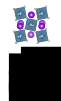
\includegraphics[width=\textwidth]{./data/plots/anharmonicity/2_materials/both.pdf}
	\caption{
		\label{fig:KCaF3}
		KCaF$_3$ in the low-temperature Pnma~(top) and high-temperature cubic phase~(bottom). Both structures are viewed along the long $b$-axis.
	}
	\label{fig:anh.KCaF3}
\end{marginfigure}

\newthought{Furthermore, it is instructive to evalute the anharmonicity for single configurations}, be it snapshots in time during molecular dynamics simulations, or when using other sampling approaches,~e.\,g,~harmonic Monte Carlo samples as defined in Eq.\,\eqref{eq:ha.samples}. The sample-resolved anharmonicity is given in analogy to Eq.\,\eqref{eq:sigmaA} as
\begin{align}
	\sigmaA [{\bf R}]
		= \sqrt{\frac{\sum_{I, \alpha} (F^{\rm A}_{I, \alpha})^2}{\sum_{I, \alpha} {(F_{I, \alpha})^2}}}~.
	\label{eq:sigmaA.sample}
\end{align}
While we will discuss ``time-resolved anharmonicity'' in detail at a later point, we show the evaluation of $\sigmaA$ for samples generated by Eq.\,\eqref{eq:ha.samples} in Fig.\,\ref{fig:anh.sampling}.
\begin{figure}
	\includegraphics[width=4.1in]{./data/plots/anharmonicity/7_sampling/convergence_sigma_MC.pdf}
	\caption{
			Anharmonicity measure $\sigmaA$ evaluated for individual atomic configurations obtained from Eq.\,\eqref{eq:ha.samples}. Dots: $\sigmaA [{\bf R}_n]$ for individual samples; Red line: Cumulative average.	Black dashed line: $\sigmaA$ from \emph{ai}MD.	Shadowed region: Convergence estimated by standard error.
	}
	\label{fig:anh.sampling}
\end{figure}
The analysis shows that a decent estimate of the anharmonicity measure $\sigmaA$ can be obtained from the harmonic sampling analysis with few samples. Especially in silicon, each individual harmonic sample yields a $\sigmaA$ within 99\,\% of the reference value obtained by MD simulations for several hundred simulation time steps, which is indicated by the dashed vertical line. For the more anharmonic KCaF$_3$, the harmonic sampling with 30~samples yields an estimated value of $\sigmaA_{\rm est.} = 0.38$, which differs from the MD value ($\sigmaA = 0.36$) by about 5\,\%. A distinction between largely harmonic materials like silicon, and anharmonic materials like KCaF$_3$, is therefore possible with very few samples.

\newthought{Motivated by this fact, we investigated the possiblity to estimate $\sigmaA$ based on a single sample}, as suggested by Zacharias and coworkers in Ref.\,\cite{Zacharias2016}, where a single, deterministic sample probing the most probable part of the harmonic distribution is used by choosing $\zeta_s = (-1)^s$ instead of a random distribution in Eq.\,\eqref{eq:ha.samples}. We denote anharmonicity measures obtained by such a ``one-shot'' approach by $\sigmaAOS$ in the following. As shown in Fig.\,\ref{fig:anh.one-shot}, the one-shot samples provide very good estimates for silicon in the the entire temperature range from 200\,K to 800\,K, which can be expected due to the largely harmonic nature of silicon.
\begin{figure}
	\includegraphics[width=4.1in]{./data/plots/anharmonicity/7_sampling/sigma_temp_one_shot.pdf}
	\caption{
		$\sigmaA$ as a function of temperature obtained from MD~simulations (black circles) and one-shot sampling (triangles connected by dashed curves)
	}
	\label{fig:anh.one-shot}
\end{figure}
For KCaF$_3$, the agreement is good in the temperature range from 200\, to 400\,K, at least within the limits of the harmonic sampling approach as discussed in the previous paragraph, taking into account that only a single sample was used. Above 500\,K, however, the difference to the reference value from MD simulations increases, which is due to the phase transition mechanism in KCaF$_3$ discussed earlier: This phase transition also occurs in the simulation cell. A prediction of anharmonicity across phase transitions therefore cannot be expected from simple harmonic sampling approaches, because the entire reference frame for the harmonic model changes when a phase transition occurs. The phase transition mechanism of KCaF$_3$ and implications for the anharmonicity measure are further discussed in Ref.\,\cite{Knoop2020}.

\newthought{Ultimately, the applicability of the one-shot sampling approach} needs to be assessed for a diverse set of materials, especially if one aims to use this scheme to screen for anharmonicity in material space. As shown in Fig.\,\ref{fig:anh.screening} for a set of 63~materials, the one-shot sampling is reliable within $\pm 10\,\%$ for all materials in the set, up to a value of about $\sigmaA \simeq 0.3$.
\begin{figure}
	\includegraphics[width=4.1in]{./data/plots/anharmonicity/8_screening/sigma_os_md.pdf}
	\caption{
		Comparison of the anharmonicity measure obtained from MD simulations and one-shot sampling (OS) for 63 materials at 300\,K. The set comprises 25 rock salt (RS), 21 zincblende (ZS), 7 wurtzite (WZ), and 10 orthorombic perovskite (Perov.) materials. The diagonal line denotes perfect agreement between MD and OS, and the green area denotes a 10\,\%~error margin to guide the eye.
		Data was taken from Ref.\,\cite{Knoop2020}.
	}
	\label{fig:anh.screening}
\end{figure}
For larger values of $\sigmaA$, the deviation can become larger, especially for the rock salt materials with $\sigmaA \simeq 0.35$ where the one-shot sampling overestimates $\sigmaA$ by about 20\,\%. Nevertheless, the agreement is qualitatively correct up to values of about $\sigmaA \simeq 0.5$, after which materials begin to show effects not captured by the harmonic sampling,~e.\,g.,~phase transitions as discussed earlier for KCaF$_3$. In particular, the three highlighted noble metal halides AgBr, CuCl, and CuBr deviate strongly. These materials tend towards non-perturbative effects during the MD simulation such as spontaneous defect formation~\cite{Knoop2020}, which is a dynamical effect impossible to be described by any reference harmonic model. We will discuss the nature of these effects in more detail later. To conclude, we point out that also in the case of non-trivial dynamical effects such as defect formation, the estimated anharmonicity scores $\sigmaAOS$ are larger than $\gtrapprox 0.5$, and therefore indicate strong anharmonicity. A qualitative classification of strong anharmonicity in terms of one-shot sampling is therefore possible for all materials in the set, while quantitative agreement is only achieved for harmonic materials with $\sigmaA \lesssim 0.2$.


\section{Anharmonicity and thermal conductivity}
\label{sec:kappa_vs_sigmaA}

Based on the qualitative discussion of thermal transport in Sec.\,\ref{sec:hf.kappa.ha}, one can expect that stronger anharmonicity leads to shorter phonon lifetimes and therefore lower thermal conductivity. We tested this hypothesis for a list of 47 materials where experimental reference was available~\cite{morelli2006,Chen2019}. The results are shown in Fig.\,\ref{fig:anh.kappa}.
\begin{figure}
	\includegraphics[width=4.1in]{./data/plots/anharmonicity/9_kappa/sigma_vs_kappa.pdf}
	\caption{
		Experimental thermal conductivity at room temperature, $\kappa^{\rm exp}_{300\,{\rm K}}$, versus one-shot measure of anharmonicity, $\sigmaAOS$. The dashed diagonal line indicates a power law fit for the data. The grey area denotes values of $\kappa$ which agree with the fit within an order of magnitude. The dataset contains 47 materials, 22 rock salt (RS), 19 zincblende (ZB), and 6 wurtzite (WZ) structures. Experimental data from Ref.~\cite{morelli2006,Chen2019}.
	}
	\label{fig:anh.kappa}
\end{figure}
The analysis reveals an inverse power law relationship between thermal conductivity and anharmonicity for the materials in the dataset. Given that just a single descriptor was used,~i.\,e.,~the estimated anharmonicity score, and no further vibrational properties as commonly employed in semi-empirical models for thermal condcutivity\CITE{Curtarolo,Toberer,Ramprasad}, this observation is somewhat surprising. At the same time, the inverse correlation is an indication that $\sigmaA$ indeed captures some essential physics relevant to heat transport.

\newthought{The most important messages from Fig.\,\ref{fig:anh.kappa} can be summarized as follows}, adopting the definition suggested by Morelli and Slack to define ``high thermal conductivity'' as $\kappa \gtrsim 50 \, {\rm W/mK}$~\cite{morelli2006}:
\begin{enumerate}
	\item Largely harmonic materials with $\sigmaA \simeq 0.1$, like diamond (C), boron nitride (BN), or boron phosphide (BP) can be expected to be good thermal conductors with $\kappa \gtrsim 100\,{\rm W/mK}$.
	\item Strongly anharmonic materials with $\sigmaA \gtrsim 0.3$ can be expected to be poor thermal conductors with $\kappa \lesssim 10\,{\rm W/mK}$.
	\item $\sigmaA$ has a strong correlation with thermal conductivity across the entire dataset, but nevertheless only a rough estimate can be made solely based on $\sigmaA$, especially in the middle region with $\sigmaA \simeq 0.2$. This can be seen by comparing strontium oxide (SrO) with $\kappa = 10\,{\rm W/mK}$ and $\sigmaA = 0.22$, and zinc oxide (ZnO) with $\kappa = 60\,{\rm W/mK}$ and $\sigmaA = 0.24$, or beryllium oxide (BeO) with $\kappa = 370\,{\rm W/mK}$ and $\sigmaA = 0.16$ to magnesium oxide (MgO) with $\kappa = 60\,{\rm W/mK}$ and $\sigmaA = 0.18$. These pairs of materials differ only slightly in their estimated anharmonicity, but still quite strongly in the thermal conductivity. 
\end{enumerate}

\newthought{These findings suggest the following approach} towards screening material space in search for thermal insulators: Estimate the anharmonicity for materials of interest and discard the largely harmonic ones, as they will be good thermal conductors most of the time. Of course, the reverse approach can be pursued when searching for materials with potentially high thermal conductivity.

\section{Candidate Materials}
\begin{marginfigure}
	\includegraphics[width=\textwidth]{./data/plots/dataset/pies.pdf}
	\caption{
		Lattice types and space groups represented in the dataset. Space groups not shown in the pie chart: 56, 61, 160, 164, 206, with one representative each.
	}
	\label{fig:anh.pie}
\end{marginfigure}
In the context of the work published in Ref.\,\cite{Knoop2020}, we have identified a set of 118 binary and ternary materials for further investigation with the \emph{ab intio} Green Kubo (aiGK) approach. The materials comprise five lattice types and 12 space groups as summarized in Fig.\,\ref{fig:anh.pie}.
%\begin{figure}
%	\includegraphics[width=\textwidth]{./data/plots/dataset/pies_horizontal.pdf}
%	\caption{
%		Lattice types and space groups represented in the dataset. Space groups not shown in the pie chart: 56, 61, 160, 164, 206, with one representative material each.
%	}
%	\label{fig:anh.pie}
%\end{figure}
Since we are mainly interested in thermal insulators as candidate thermoelectric and thermal barrier coating materials, we have discarded largely harmonic materials with $\sigmaA < 0.17$ from the set, and focus on anharmonic strengths $\sigmaA > 0.2$ with a mean of $\sigmaA=0.31$ and a median of $\sigmaA = 0.29$. A histogram displaying the distribution of $\sigmaA$ values is shown in Fig.\,\ref{fig:anh.histogram}.
\begin{figure}
	\includegraphics[width=4.1in]{./data/plots/dataset/histogram.pdf}
	\caption{
		Histogram of $\sigmaAOS$ values samples for the 118 chosen materials
	}
	\label{fig:anh.histogram}
\end{figure}
All values are given with respect to room temperature, as this is the regime where the most experimental reference is available to benchmark the aiGK method and to showcase the approach. In total, there are experimental reference values for 45 materials available, were we have discarded sources of questionable quality.

\REM{
The materials come from these sources:
From Ramprasad: 41
From Toberer: 3
From Springer: 4
From Roekeghem: 9
From ICSD: 55
From Seko: 2
From AAPL: 4
}

\TODO{Include materials with reference in appendix}

\newpage
\section{Dynamical effects}
As shown in the initial screening of material space presented in Ref.\,\cite{Knoop2020}, strongly anharmonic materials with $\sigmaA > 0.3$ are prone to exhibiting non-trivial dynamical effects such as metastable defect formation and precursors of structural phase transitions. 

\newthought{We carried out \emph{ab initio} molecular dynamics simulations}~\footnote{Computational settings: PBEsol function and \emph{light default} basissets. Time step 4-5\,fs based on the highest harmonic vibrational frequency, total simulation time at least 30\,ps. Lattice expansion accounted for by minimizing the pressure in the simulation cell according to the scheme outlined in Sec.\,\ref{sec:app.lattice_expansion}. Full details given in appendix \ref{sec:app.computational_details}.} for each of the candidate materials introduced in the previous chapter to see whether the materials exhibit such non-trivial dynamical effects. 
These dynamical effects can be detected by using a time-resolved anharmonicity measure as defined in Eq.\,\eqref{eq:sigmaA.sample},~i.\,e.,~by evaluating the anharmonicity measure for each sample during the MD with $\sigmaA(t) = \sigmaA [{\bf R} (t)]$, and evaluating fluctuations of $\sigmaA (t)$ in terms of its standard deviation ${\rm std} [ \sigmaA ]$ evaluated along a given trajectory. A comparison of $\sigmaA$ values obtained by one-shot sampling, $\sigmaAOS$, and molecular dynamics, $\sigmaAMD$, is shown in Fig.\,\ref{fig:sigma_os_md_dataset}. Materials with a standard deviation larger than ${\rm std} [ \sigmaAMD ] > 0.01$ are highlighted and labeled.
\begin{figure}
	\includegraphics[width=4.1in]{./data/plots/sigma_vs_sigma/sigma_os_md_edit.pdf}
	\caption{$\sigmaA$ values obtained by one-shot sampling (OS) and molecular dynamics simulations (MD) in comparison. Materials with significant fluctuations of the time-resolved anharmonicity measure $\sigmaA (t)$ are highlighted and labeled.}
	\label{fig:sigma_os_md_dataset}
\end{figure}
We discuss the nature of these effects for KCaF$_3$, CuI, AgI, and AgCl in the following. AgBr and KCdF$_3$ are omitted because they behave qualitatively similar to AgCl and KCaF$_3$, respectively. 

The discussion is meant to highlight the prevalence of non-trivial dynamical effects that violate one basic assumption of phonon theory,~i.\,e.,~the assumption of well-defined and stationary reference positions for all atoms in a given phase. Another key insight is that the observed effects are precursors of phase transitions known to occur in these materials at higher temperatures, which means that their onset is observed on the microscopic scale during the dynamic evolution already several 100\,K below the phase transition temperature.
From a methodological point of view, we show how the time-resolved anharmonicity can be used to uncover and explain the nature of the underlying dynamical effect.

\newpage

\subsection{KCaF$_3$}
KCaF$_3$ is the perovskite material already discussed in some detail in Sec.\,\ref{sec:anharmonicity_measure}, where the octahedral tilting mechanism typical for this class of materials, and the phase transition phenomenology were presented~\cite{Bulou1980,Hidaka1984,Knight2005}. In total, we performed five $NVE$ simulations for KCaF$_3$, with a simulation time of 30\,ps each. The time resolved anharmonicity measure is displayed for each of those trajectories in Fig.\,\ref{fig:defects.KCaF3.sigmaA}.
We find that in three of the five trajectories, $\sigmaA (t)$ jumps between the reference values of $\sigmaA \approx 0.4$,\footnote{We round to 1 decimal point in the following, which is completely sufficient for the discussion of intermittent jumps.} and increased values between $\sigmaA \approx 0.8$ and $\sigmaA \approx 1.2$.
%
\begin{figure}
	\includegraphics[width=\textwidth]{./data/plots/defects/062.05.KCaF3/sigma_vs_time.pdf}
	\caption{Time-resolved anharmonicity measure $\sigmaA (t)$ for orthorombic KCaF$_3$ in five molecular dynamics runs or 30\,ps length. Increased values of $\sigmaA (t)$ are found in three trajectories (b, d, e).}
	\label{fig:defects.KCaF3.sigmaA}
\end{figure}
%
\newthought{The nature of the underlying dynamical effects} can be resolved by time-averaging the positions ${\bf R} (t)$,
\begin{align}
	{\bf R}_{\rm avg} = \braket{{\bf R} (t)}_t~,	
	\label{eq:R(t).avg}
\end{align}
%
\begin{marginfigure}[-3cm]
	\includegraphics[width=\textwidth]{./data/plots/defects/062.05.KCaF3/plots/ref_left.png}
	\includegraphics[width=\textwidth]{./data/plots/defects/062.05.KCaF3/plots/2_left.png}
	\includegraphics[width=\textwidth]{./data/plots/defects/062.05.KCaF3/rdf/geometry_in_def_2.pdf}
	\caption{Precursor of phase transition in KCaF$_3$. Upper panel: The reference orthorombic structure viewed in (010) direction. The orthorombic displacement of the potassium sub-lattice (violet balls connected by sticks) is clearly visible. Middle panel: When $\sigmaA (t) \approx 1.1$, the potassium sub-lattice temporarily adopts a tetragonal shape. Also the fluorite atoms (small blue balls) reduce their tilt consequently. Lower panel: Radial distribution function $g(r)$ for the fluorine atoms in the orthorombic reference and deformed structure: The number of distinct peaks reduces, reflecting an increase in symmetry when the orthorombic tilt reduces.}
	\label{fig:defects.KCaF3.1}
\end{marginfigure}
\noindent
for the time spans where $\sigmaA (t)$ is increased. Performing this time average for time spans where $\sigmaA (t) < 0.5$,~i.\,e.,~in situations where no increase is seen, one recoveres the initial orthorombic structure shown in Fig.\,\ref{fig:defects.KCaF3.1} (top figure). When averaging trajectory b) for the time where $\sigmaA (t) \approx 1.1$, the resulting structure is more symmetric, with an approximately tetragonal arrangement of atoms. This can be seen by focusing on the potassium sub lattice (purple atoms connected by sticks) in Fig.\,\ref{fig:defects.KCaF3.1} (middle). The increased symmetry is further revealed by noting that the fluorine cage becomes more ordered, as shown in terms of the F-F pair distribution function in Fig.\,\ref{fig:defects.KCaF3.1} (bottom). This phenomenon can be viewed as a precursor of the phase transitions towards tetragonal and cubic phases known to occur in the material at temperatures higher than 560\,K~\cite{Bulou1980,Hidaka1984,Knoop2020}. However, at 300\,K, well below the transition temperature, this configuration only occurs sporadically on the time scale of several picoseconds during the simulation, and is therefore not fully stabilized.

% \newpage

\subsection{CuI}
\label{sec:defects.CuI}

\begin{figure}
	\includegraphics[width=\textwidth]{./data/plots/defects/216.02.CuI/sigma_vs_time.pdf}
	\caption{Zincblende (SG\,216) CuI, describe comp. details}
	\label{fig:defects.CuI}
\end{figure}
\noindent
Copper iodide (CuI), also known as marshite, is a simple material with fcc lattice of the zincblende type. This phase is also known as the $\gamma$ phase ($\gamma$-CuI).
The time-resolved anharmonicity measures are shown in Fig.\,\ref{fig:defects.CuI} for three trajectories of 60\,ps simulation time.
The characteristic features are the jumps in $\sigmaA (t)$ from values of $\sigmaA (t) \approx 0.5$ to $\sigmaA (t) \approx 1.2$ or 1.6. In the simulated time period, these values are taken for 3 to 12\,ps, before the initial value of $\sigmaA (t) \approx 0.5$ is restored. 
% The jumps in $\sigmaA (t)$ hint at a dynamical effect which strongly violates the harmonic approximation.
%
\begin{marginfigure}
	\includegraphics[width=\textwidth]{./data/plots/defects/216.02.CuI/all.pdf}
	\caption{CuI viewed in (110) direction. Top: High-symmetry zincblende structure. Middle: Copper ion in lower-right quadrant moves into interstitial site along (111) direction when $\sigmaA (t) \approx 1.2$. Bottom: Several defects form when $\sigmaA (t) \approx 1.6$}
	\label{fig:defects.CuI.1}
\end{marginfigure} 
%
As in the case of KCaF$_3$, we compare two time-averaged structures in Fig.\,\ref{fig:defects.CuI.1}: A time average with respect to the entire simulation time reveals the perfect zincblende structure of CuI which corresponds to the minimum of the potential energy surface.
When averaging over the time span where $\sigmaA (t) \approx 1.2$, however, the average structure has one Cu atom diplaces along the (111) direction. Viewing the supercell in (110) direction, the diplacement is clearly visible (Fig.\,\ref{fig:defects.CuI.1}, middle). This means that the Cu occupies a metastable interstitial site at the given position for the respective time period. When $\sigmaA (t)$ is restored to the base value of $\sigmaA (t) \approx 0.5$, the Cu atom moves back to the high-symmetry reference position within the zincblende structure. 
The third trajectory shown in Fig.\,\ref{fig:defects.CuI}~c) evolves to a situation where $\sigmaA \approx 1.6$. This corresponds to a situation, where more than one defects forms~(Fig.\,\ref{fig:defects.CuI.1}, bottom).

\newthought{$\gamma$-CuI is known to undergo a phase transition to a superionic conducting $\beta$ phase} above 643\,K~\cite{boyce1979, boyce1980,boyce1981,keen1995}. It is very likely that the defect formation observed in the aiMD simulations at 300\,K are precursors of this phase transition, but too infrequent at this temperature to destabilize the fcc lattice of the $\gamma$ phase.
\TODO{cation size}


\subsection{AgI}
Wurtzite silver iodide ($\beta$-AgI), or iodargyrite, is another transition metal halide that shares some similarities with $\beta$-CuI discussed in the previous section~\cite{boyce1981}. It is known to transition into the superionic conducting $\alpha$ phase above $\sim 420$\,K~\cite{hoshino1957,boyce1981,Brenner2020}, and was in fact one of the earliest studied materials exhibiting this phenomenon~\cite{strock1934,strock1935,strock1936}.
%
\begin{figure}
	\includegraphics[width=\textwidth]{./data/plots/defects/186.02.AgI/sigma_vs_time.pdf}
	\caption{Wurtzite (SG\,186) AgI, describe comp. details}
	\label{fig:defects.AgI}
\end{figure}
%
\begin{marginfigure}
	\includegraphics[width=\textwidth]{./data/plots/defects/186.02.AgI/defects_all.png}
	\caption{AgI viewed in (100) direction. Top: High-symmetry wurtzite structure. Middle: Silver ions (red) move into interstitial sites along (001) direction when $\sigmaA (t) \approx 1.3$. Bottom: The same configuration viewed along (001) direction.}
	\label{fig:defects.AgI.1}
\end{marginfigure} 
%
The time-resolved anharmonicity measure for AgI at 300\,K is shown in Fig.\,\ref{fig:defects.AgI}. As in $\gamma$-CuI, the value jumps back and forth between the already quite large reference value of $\sigmaA \approx 0.7$, short spikes at $\sigmaA \approx 0.5$, and longer periods where $\sigmaA \approx 1.3-1.6$ for several picoseconds. For example, the first trajectory displayed in Fig.\,\ref{fig:defects.AgI}~a) jumps between $\sigmaA \approx 0.7$ and $\sigmaA \approx 1.3$ several times, where the longest time span around this value is about 5\,ps. Averaging the positions over this time span as before, we obtain a supercell containing three Ag defects moving along (001) direction in the supercell, as shown in Fig.\,\ref{fig:defects.AgI.1} (middle and bottom), as opposed to the reference wurtzite structure (top).
It is again very likely that the instability of the wurtzite lattice towards defect formation at room temperature is a precursor of the actual phase transition taking place at temperatures approximately 120\,K higher. 

\newpage
\subsection{AgCl}
Silver chloride (AgCl) is yet another material of the class of transition metal halides, and the room-temperature stable phase is rock salt~\cite{lowndes1972,andreoni1983,batchelor1995}.
\begin{figure}
	\includegraphics[width=\textwidth]{./data/plots/defects/225.02.AgCl/sigma_vs_time.pdf}
	\caption{Rocksalt (SG\,225) AgCl, describe comp. details}
	\label{fig:defects.AgCl}
\end{figure}
%
\begin{marginfigure}[-2in]
	\includegraphics[width=\textwidth]{./data/plots/defects/225.02.AgCl/per_atom/histogram_atoms_margin.pdf}
	\caption{Species-resolved anharmonicity score in AgCl.}
	\label{fig:defects.AgCl.sigmaA}
\end{marginfigure}
%
As opposed to the previously discussed transition metal halides CuI and AgI, the time-resolved anharmonicity $\sigmaA (t)$ exhibits no ``jumps'' in AgCl, but rather stays constants at $\sigmaA \approx 1$, which can be interpreted as a situation where the 0\,k harmonic model loses predictive power for the observed forces. By resolving the anharmonicity measure per atom species in Fig.\,\ref{fig:defects.AgCl.sigmaA} similar to the discussion for KCaF$_3$ in Sec.\,\ref{sec:anharmonicity_measure}, we see that the harmonic model performs better for the chlorine atoms with $\sigmaA_{\rm Cl} = 0.86$, and worse for silver with $\sigmaA_{\rm Ag} = 1.25$. This is in line with the previous observations in metal halides where small cations proved to be more mobile and susceptible to dislocations. However, no clear-cut dislocation pattern can be identified for AgCl as opposed to CuI and AgI.
%
\begin{figure}
	\centering
	\includegraphics[width=3.5in]{./data/plots/pdfs/agcl.pdf}
	\caption{Rocksalt (SG\,225) AgCl, describe comp. details
	Coordination shells: 
	1: 2.75579 atoms: Cl-Ag 
	2: 3.89727 atoms: Ag-Ag/Cl-Cl 
	3: 4.77317 atoms: Ag-Cl 
	4: 5.51158 atoms: Ag-Ag	
}
	\label{fig:defects.pdf.agcl}
\end{figure}
%
\newthought{The nature of the dynamical effects manifesting in AgCl can nevertheless be elucidated.} We do this by computing the pair distribution functions for the first four coordinates shells in AgCl
\CITE{pair distribution function. Boon?}
, as shown in Fig.\,\ref{fig:defects.pdf.agcl}, and contrasting them with the prototypical, largely harmonic rock salt material magnesium oxide (MgO, $\sigmaA = 0.17$) in Fig.\,\ref{fig:defects.pdf.mgo.small}. 
%
\begin{marginfigure}
	\includegraphics[width=\textwidth]{./data/plots/pdfs/mgo_small.pdf}
	\caption{Radial distribution function resolved by pair contributions.}
	\label{fig:defects.pdf.mgo.small}
\end{marginfigure}
%
In MgO, the distribution of atoms are sharply distinguishable, which means that the atoms vibrate closely around their reference position. In AgCl on the other hand, only the first coordination shell of silver-chlorine atoms is distinct at 300\,K. The chlorine (Cl-Cl) and silver (Ag-Ag) sublattices (purple/green area in Fig.\,\ref{fig:defects.pdf.agcl}) show discernible peaks, although the broadening is significant compared to MgO. The silver-chlorine (Cl-Ag) distribution (yellow area) is even more broadened and is still non-zero at distances normally characteristic of like atoms (Cl-Cl or Ag-Ag) , see~e.\,g.,~the non-zero width of the yellow curve at 3.9 and 5.5\,\AA (second and fourth coordination shell). In total, this leads to a very strong broadening in the third and fourth coordination shell, with a barely discernible local maximum in the third coordination shell (4.8\,\AA).
This is in line with experimental Extended X-ray Absorption Fine Structure (EXAFS) measurements detecting an ``anomalously large motion'' in the third neighbor shell already at a temperature of 120\,K~\cite{batchelor1995}.
This hints at severe dynamical distortions throughout the simulation which are typically discussed in terms of dynamical Frenkel pair formation, where the mobile Ag$^+$ cations dynamically populate interstitial sites~\cite{Aboagye1975,andreoni1983,wilmer1995,mebane2010}. While we can confirm an increased mobility of Ag$^+$ ions as discussed above, we do not observe a local accumulation of Ag$^+$ ions at interstitial sites, which should correspond to additional local minima in the respective pair distribution functions compared to the reference structure. However, such an effect might very well occur at higher temperatures, and the observed effects are fingerprints of the instability of the lattice towards this kind of dynamical defect formation.
Irrespective of the exact type of defect formation, %which is beyond the scope of this work, 
the observed dynamical effects hint at a strong form of premelting phenomenon in AgCl, which has an experimental melting temperature of 728\,K.

\newthought{Similar effects can be observed in silver bromide (AgBr)}. As discussed in Ref.\,\cite{andreoni1983}, the dynamical properties of AgCl and AgBr share many similarities with the chemically related material AgI presented in the previous section. In contrast to AgI however, they do not become superionic conductors before melting, despite the increased ion mobility presented here.


\subsection{Conclusion}
In summary, we have observed a variety of non-perturbative dynamical effects occuring in the candidate materials, and discussed them for the prototypical systems KCaF$_3$, $\gamma$-CuI, $\beta$-AgI, and AgCl. The common feature of these effects is that they indicate phenomena which are known to occur in the respective materials, but at significantly higher temperatures. This comprised the onset of structural phase transitions in KCaF$_3$, fingerprints of a superionic phase in CuI and AgI, and pre-melting phenomena in AgCl and AgBr.



\chapter{Ab Initio Green Kubo: Implementation}
\label{chp:implementation}

The theoretical background for the \emph{ab initio} simulation of thermal conductivity has been established in the previous chapters, in particular, Chp.~\ref{chp:heat_transport}. The purpose of this chapter is to discuss the practical implementation of the respective formulas for two benchmark materials. The scheme is implemented in FHI-vibes~\cite{FHI-vibes}.

\newthought{We restate the Green-Kubo formula} for the thermal conductivity initially introduced in Sec.\,\ref{sec:ab_initio_heat_flux} as
\begin{align}
	\kappa^{\alpha \beta} (T)
		= \int \d \Gamma_0 ~ \kappa^{\alpha \beta} (\Gamma_0) f_T (\Gamma_0) ~,
	\label{eq:implementation.kappa.avg}
\end{align}
where $\kappa^{\alpha \beta} (T)$ are the Cartesian components of the thermal conductivity tensor at temperature $T$,\footnote{$T$ represents all thermodynamic conditions in the simulation, including pressure $p$.} and $\Gamma_0$ are phase-space configurations with a respective ensemble weight $f_T (\Gamma_0)$ at the given temperature. For each phase-space configuration $\Gamma_0$, the thermal conductivity is computed as
\begin{align}
	\kappa^{\alpha \beta} (\Gamma_0)
		&=
		\frac{V}{k_{\rm B} T^2} 
		\lim_{t_{\rm c} \to \infty}
		\int_{0}^{\tcut} 
		\d t ~ C_{JJ}^{\alpha \beta} (\Gamma_0, t)~.
	\label{eq:implementatino.kappa.1}
\end{align}
Here, $	C^{\alpha \beta}_{J J} (\Gamma_0, t)$ denotes the heat flux autocorrelation function (HFACF),
\begin{align}
	C^{\alpha \beta}_{J J} (\Gamma_0, t)
		=
		\lim_{t_{0} \to \infty}
		\frac{1}{t_0 - t}
		\int_{0}^{t_{\rm 0} - t} 
		\d s ~ J^\alpha (\Gamma_{t + s}) J^\beta (\Gamma_s)~,
	\label{eq:implementatino.acf.1}
\end{align}
which can be viewed as an average over all available starting conditions $\Gamma_s$ during a simulation of length $t_0$. Each phase-space point $\Gamma_t$ is related to the initial configuration $\Gamma_0$ through the canonical time evolution determined by the many-body Hamiltonian of the system, $\mathcal H (\Gamma)$. Equation~\eqref{eq:implementation.kappa.avg} through~\eqref{eq:implementatino.acf.1} represent an exact reformulation of the Green Kubo formula.


\newthought{In order to evaluate these equations in finite simulations}, the integrals need to be discretized and truncated to finite domains. First, we approximate Eq.\,\eqref{eq:implementation.kappa.avg} by choosing a finite set of $M$ starting configurations $\Gamma_0^i$, so that
\begin{align}
	\kappa^{\alpha \beta} (T)
		\approx
		\frac{1}{M} \sum_{i=1}^M \kappa^{\alpha \beta} (\Gamma_0^i)~,
	\label{eq:implementation.kappa.mean}
\end{align}
where the starting conditions $\Gamma_0^i$ are chosen from NVT molecular dynamics simulations for the thermodynamic conditions of interest. For each starting condition $\Gamma_0^i$, we perform NVE molecular dynamics simulations to generate the time evolution of the system, $\Gamma_t^i$, 
%\mscomment{you don't need initial equilibration?}
%\FK{All convergence checks go by discarding the first time period, I didn't see an effect there when discarding a few ps. I think it really depends on the quantity one is interest in. Also it's often a minor error compared to things like energy drift in aiMD runs, I would guess.}
and evaluate the heat flux, $J^\alpha (\Gamma_t^i)$ along this trajectory. The simulation is performed for a total simulation time $t_0$, thereby truncating the time integral in Eq.\,\eqref{eq:implementatino.acf.1}. From the resulting autocorrelation function of finite length, the thermal conductivity is computed via Eq.\,\eqref{eq:implementatino.kappa.1}, where a \emph{cutoff time} $\tcut < t_0$ is chosen to avoid integrating parts of the autocorrelation function after it has effectively decayed, as non-zero values are only due to statistical fluctuations stemming from finite size and time effects~\cite{Jones.2012}.
%\mscomment{what noise?}
%\FK{statistical noise in the ACF due to finite size/finite time scales. Not fully balances statistical distribution of phonon modes, etc}
After computing the thermal conductivity for each trajectory, the final value is given by Eq.\,\eqref{eq:implementation.kappa.mean},~i.\,e.,~by the \emph{mean} of the individual trajectories. The statistical error due to the finite ensemble average is estimated by the \emph{standard error},~i.\,e.,~the standard deviation of the mean,
\begin{align}
	\Delta \kappa^{\alpha \beta} (T)
		= \frac{1}{\sqrt{N}} \sqrt{\frac{1}{N} \sum_i \left( \kappa^{\alpha \beta} (T) - \kappa^{\alpha \beta} (\Gamma_0^i) \right)^2}~.
	\label{eq:imp.kappa.err}
\end{align}
From the Cartesian components of the thermal conductivity $\kappa^{\alpha \beta} (t)$, the scalar thermal conductivity $\kappa (T)$ is obtained via
\begin{align}
	\kappa (T)
		= \frac{1}{3} \sum_{\alpha} \kappa^{\alpha \alpha} (T)~.
	\label{eq:kappa.scalar}
\end{align}


\newthought{In empirical force field approaches}, the appearing equations can be evaluated as is, and convergence in size and time can be checked in a brute-force way by increasing the respective scales well beyond the necessary limits.
%\CITE{Lammps, Jones, more}. 
From an \emph{ab initio} perspective, the accessible size and time scales are each at least two orders of magnitude lower,\footnote{Force fields: 1\,ns for 10000~atoms within 1 day on one supercomputer node, \emph{ab initio}: 50\,ps for 200~atoms within 1~months on five supercomputer nodes.} and additional steps are necessary to increase the amount of information that can be extracted from the comparatively short simulations. The purpose of this chapter is to discuss these additional steps in detail: First, we present steps to remove noise from the heat flux autocorrelation functions $C_{JJ} (t)$, which enables to choose cutoff times $\tcut$ in a numerically robust way. Next, we discuss the size extrapolation scheme in terms of the harmonic mapping presented in Sec.\,\ref{sec:aiGK} which allows to correct for the finite size of simulations cells used in \emph{ab initio} molecular dynamics simulations. Finally, we discuss the necessary simulation times $t_0$ and how those can be estimated for novel materials.

\newthought{We present the implementation in detail} for the case of periclase magnesium oxide (MgO) which is well-known in the literature, and, as a rather harmonic material, a typical benchmark system for perturbative heat transport techniques. We then apply the same approach to the strongly anharmonic marshite copper iodide (CuI), for which basic assumptions of perturbation theory are violated, as we will explain in detail. 
Both structures are studied at GGA level of theory using the PBEsol functional and light-default basissets in FHI-aims~\cite{Perdew.2008,FHI-aims}. Supercell sizes are 216 atoms each, and the MD simulations are performed via FHI-vibes~\cite{Larsen.2017,FHI-vibes}. The aiGK methods as described is implemented in FHI-vibes as well. Force constants for the size extrapolation via harmonic mapping are obtained via regression from the MD runs via the temperature dependent effective potentials code (TDEP)~\cite{Hellman.2013}.\footnote{See also appendix~\ref{app:force_constants}.} The MD runs are thermalized using the pre-thermalization technique outlined in Sec.\,\ref{sec:harmonic_sampling} using finite-differences force constants obtained via phonopy~\cite{phonopy}. Afterwards, a Langevin thermostat at the target temperature (300\,K) is used to perform NVT sampling. After and initial sampling period of 2.5\,ps, the thermal pressure is relaxed according to the scheme outlined in Sec.\,\ref{sec:app.lattice_expansion} in the appendix to account for thermal expansion. Starting points $\Gamma^i_0$ for the NVE simulations are chosen from an NVT run for the relaxed supercell at least 2\,ps apart. The time step for the MD simulation was chosen as 5\,fs, which corresponds to a tenth of the shortest period duration of the harmonic spectrum of MgO ($\omega_{\rm max} \approx 20$\,THz).


\section{Noise reduction scheme and cutoff estimation}
\subsection{Discard non-contributing terms}
The raw \emph{ab initio} heat flux used in this work was defined in Eq.\,\eqref{eq:J_ai} and is given for a phase-space point $\Gamma_t = \set{{\bf R} (t), \dot{{\bf R}} (t)}$ by
\begin{align}
	{\bf J}^{\rm raw} (t) 
		= \frac{1}{V} \sum_I \sigma_I (t)  \dot{{\bf R}}_I (t)~,
	\label{eq:imp.J.0}
\end{align}
where $\sigma_I (t) \equiv \sigma_I [{\bf R} (t)]$ are atomic virial tensors for the configuration at the given time $t$ as defined in Eq.\,\eqref{eq:hf.sigma_I}, and $\dot{{\bf R}}_I (t)$ is the velocity of atom $I$ as usual. We split the raw flux in two parts,
\begin{align}
	{\bf J}^{\rm raw} (t)
		= \frac{1}{V} \sum_I \delta \sigma_I (t) \dot{{\bf R}}_I (t) 
		+ \frac{1}{V} \sum_I \braket{{\sigma_I}} \dot{{\bf R}}_I (t)~,
	\label{eq:imp.J.1}
\end{align}
where $\braket{\sigma_I}$ is the average atomic virial, and $\delta \sigma_I (t)$ is the time-dependent part. In the absence of diffusion, the second term is the total time derivative of a bounded vector field, $\sum_I \braket{\sigma_I} \dot{{\bf R}}_I (t) = \frac{\d}{\d t} \sum_I \braket{{\sigma_I}} {\bf R}_I (t)$. By means of the gauge invariance principle introduced in Sec.\,\ref{sec:gauge_invariance}, it therefore does not contribute to the time integral in Eq.\,\eqref{eq:implementatino.kappa.1}, and can be discarded before evaluating the heat flux autocorrelation function~\cite{Ercole.2016}. We therefore always use the following heat flux expression:
\begin{align}
	{\bf J} (t)
		= \frac{1}{V} \sum_I \delta \sigma_I (t) \dot{{\bf R}}_I (t)~.
	\label{eq:imp.J}
\end{align}
Depending on the material, discarding the non-contributing part from the raw heat flux reduces the noise in the simulation \emph{massively}, as shown for the case of MgO in the upper panel of Fig.\,\ref{fig:imp.hfacf.kappa.1} (orange curves compared to light blue curves).

Due to the finite time of the simulation, we furthermore enforce a vanishing expectation of the flux to remove bias from the resulting quantities by removing the finite-time average, ${\bf J} (t) \to \delta {\bf J} (t) = {\bf J} (t) - \braket{{\bf J}}_t$.
%
\begin{figure}
	\includegraphics[width=\textwidth]{./data/plots/implementation/MgO/hfacf_data_yy_3.pdf}
	\caption{Heat flux autocorrelation function $C_{JJ}(t)$ (HFACF) as defined in Eq.\,\eqref{eq:implementatino.acf.1} and its cumulative integral,~i.\,e.,~the thermal conductivity $\kappa (t)$ as function of lag time $t$. Light blue: $C_{JJ}(t)$ and $\kappa (t)$ obtained by using the raw flux as defined in Eq.\,\eqref{eq:imp.J.0}. Orange: After discarding the gauge-invariant term in Eq.\,\eqref{eq:imp.J.1}. Black curves: After applying additional, integral-preserving noise filtering as explained in the main text. The cutoff time $t_{\rm c}$ is chosen based on the ``first dip'' of the noise-filtered HFCAF.
	\emph{Computational details:} The shown data is for the $\kappa^{yy}$-component of MgO in an aiMD simulation of 60\,ps total length using a time step of 5\,fs. The heat flux was evaluated every four steps. The system was thermalized to 300\,K using a Langevin thermostat. The system size is 216 atoms in a cubic supercell.}
	\label{fig:imp.hfacf.kappa.1}
\end{figure}

\subsection{Noise filtering}
After discarding the gauge-invariant contributions from the heat flux, there is still a considerable level of noise in the HFACF, which hinders a robust identification of the time at which it is fully decayed,~i.\,e.,~the cutoff time $\tcut$. Available techniques to identify cutoff times, such as the first avalanche method introduced in Ref.\,\cite{Chen.2010}, are not fully parameter-free, and need hand tuning, even if very little.\footnote{The first avalanche technique determines cutoff times by means of a signal-over-noise ratio and relies on two parameters, a window size for computing moving averages, and a threshold value for the resulting avalanche function.} We therefore suggest an approach that does rely only on a single parameter which is chosen based on the vibrational spectrum of the material: Motivated by the fact that the \emph{integrated} HFACF,~i.\,e.,~the cumulative thermal conductivity
\begin{align}
	\kappa (t)
		=
		\frac{V}{k_{\rm B} T^2} 
		\int_{0}^{t} 
		\d t' ~ C_{JJ} (t')~,
	\label{eq:imp.kappa.cum}
\end{align}
is already a much smoother function than the HFACF itself, we apply a shape-preserving Savitzky-Golay filter to $\kappa (t)$ as implemented in Scipy~\cite{Savitzky.1964,scipy}. The remaining parameter is the window size for the filter. It is chosen based on the vibrational spectrum of the material by taking the period length corresponding to the slowest significant frequency $\omega_{\min}$. Thereby, all noise of higher frequency is effectively filtered from $\kappa (t)$, while all relevant time integrals are preserved by construction: The cumulative kappa before (orange curve) and after (black curve) lie right on top of each other in the lower panel of Fig.\,\ref{fig:imp.hfacf.kappa.1}. The filter is constructed such that the antisymmetry of $\kappa (t)$ in time, $\kappa (-t) = - \kappa (t)$ is respected.\footnote{The antisymmetry of $\kappa (t)$ is a consequence of the time symmetry of $C_{JJ} (t)$.} This also ensures that $\kappa (t)$ vanishes identically at $t=0$.

Based on the filtered cumulative thermal conductivity, the HFCAF can be obtained by differentiating, which carries over the filtering to $C_{JJ} (t)$. The filtered HFACF can be obtained analytically by fitting spline functions to $\kappa (t)$, or numerically by applying the same filter on the numerical gradient of $\kappa (t)$. The resulting cumulative thermal conductivity $\kappa (t)$ and HFACF $C_{JJ} (t)$ are shown as black curves in Fig.\,\ref{fig:imp.hfacf.kappa.1}. From the noise-filtered HFACF, the cutoff time $\tcut$ is chosen by a ``first dip'' criterion,~i.\,e.,~when $C_{JJ} (t)$ drops to zero~\cite{Chen.2010}. This corresponds to the first significant plateau in $\kappa (t)$ after removing the noise. With the cutoff time $\tcut$, the resulting thermal conductivity for a given component of the thermal conductivity tensor is given by the value $\kappa = \kappa (\tcut)$ as indicated by the dashed horizontal line in Fig.\,\ref{fig:imp.hfacf.kappa.1}.
The presented scheme will be used for all reported values of thermal conductivity in the following.

\section{Size extrapolation}
\label{sec:imp.extrapolation}

%\mscomment{tell more clearly what is new and what not}
After we have seen how the Green-Kubo formula is used to compute thermal conductivities from the \emph{ab initio} heat flux evaluated along aiMD trajectories, we shortly review the size extrapolation scheme first introduced in Ref.\,\cite{Carbogno.2016} and discussed in more detail in Sec.\,\ref{sec:aiGK}. The aim of the size extrapolation is to correct for finite size effects occuring in aiMD simulations, because the supercells used in \emph{ab initio} simulations are limited in size, and phonon modes of longer wavelength than the supercell are therefore not included. 

\newthought{As discussed in Sec.\,\ref{sec:aiGK}}, the correction works by computing the harmonic contribution to the thermal conductivity $\kappa_{\rm ha}$ within the supercell via Eq.\,\eqref{eq:ha.kappa.bte}
\begin{align}
	\kappa_{\rm ha}^{\alpha \beta} = V k_{\rm B} \sum_{b, {\bf q}} v^\alpha_b ({\bf q}) v^{\beta}_b ({\bf q}) \fD \tau_b ({\bf q})~,
	\label{eq:imp.K.bte}
\end{align}
where $v_b^\alpha ({\bf q})$ is the group velocity of a phonon mode with band index $b$ and \emph{commensurate} wave vector $\bf q$, and $\tau_b ({\bf q})$ is the lifetime obtained from the autocorrelation function of the mode-resolved energy $E_b ({\bf q}, t)$ as defined and discussed in Eq.\,\eqref{eq:G_s}~\cite{Carbogno.2016}, and shown in Fig.\,\ref{fig:G_s}. 
%
% This is exemplified for a simulation of MgO at 300\,K in Fig.\,\ref{fig:G_s}.
%
\begin{figure}
	\includegraphics[width=\textwidth]{./data/plots/lifetimes/greenkubo_summary_interpolation_lifetimes.pdf}
	\caption{Fit of mode lifetimes for MgO at 300\,K. Simulation performed with a timestep of 5\,fs for a simulation time of 60\,ps. The size of the simulatin cell was 216 atoms. Left: normalized mode-energy autocorrelation function $G_s (t)$ as obtained from the simulation by Eq.\,\eqref{eq:G_ss}. Right: Analytic expression of the form $G_s (t) = {\rm e}^{-t / \tau_s}$ after fitting mode lifetimes $\tau_s$. The y-axis is logarithmic such that exponential functions appear as straight lines.}
	\label{fig:G_s}
\end{figure}
%
For a given simulation $\set{\Gamma^i  _t}$, Eq.\,\eqref{eq:imp.K.bte} is evaluated for all commensurate $\bf q$-points, and projected to the symmetry-inequivalent points in the Brillouin zone determinded by the space group operations of the system to improve the statistics~\cite{Maradudin.1968}. The irreducible q-points in the Brillouin zone are obtained by iteratively reducing the given grid with the available symmetry operations for the system obtained by the spglib package~\cite{Spglib}.

\newthought{In the next step}, the lifetimes $\tau_b ({\bf q})$ are interpolated to denser $\bf q$-point meshes by $\fD{\tilde{\tau}}_b (\tilde{{\bf q}}) = \fD \lambda_b (\tilde{{\bf q}}) \omega_b^{-2} (\tilde {{\bf q}})$ with a weakly $\bf q$-dependent function $\lambda_b (\tilde {{\bf q}})$ obtained by linearly interpolating the lifetimes obtained at commensurate $\bf q$-points.\footnote{We use linear interpolation at variance with Ref.\,\cite{Carbogno.2016}, as we found it to be numerically more robust. However, results should not significantly depend on the interpolation algorithm used to obtain $\lambda_b (\tilde{{\bf q}})$, as the physically relevant contribution is captured by the $\omega_b^{-2} ({\bf q})$  scaling.} The scaling of lifetimes with $\omega_b^{-2} ({\bf q})$ is rooted in basic phonon theory as discussed in detail by Herring~\cite{Herring.1954}. For the acoustic modes at ${\bf q} = \Gamma = 0$, where $\omega ({\bf q \to 0}) \to 0$, the value for $\lambda_b (\Gamma)$ is obtained by averaging over values at the surrounding $\bf q$-points. For the new, denser grid, an interpolated value,
\begin{align}
	\kappa_{\rm ha - int}^{\alpha \beta} (N_{\tilde{\bf q}}) = V k_{\rm B} \frac{N_{\bf q}}{N_{\tilde{\bf q}}} \sum_{b, \tilde{{\bf q}}} v^\alpha_b (\tilde{{\bf q}}) v^{\beta}_b (\tilde{{\bf q}}) \fD{\tilde{\tau}}_b (\tilde{{\bf q}})~,
	\label{eq:imp.K.bte.correction}
\end{align}
can be obtained, where $N_{\tilde{\bf q}}$ is the number of points in the new grid, and the factor $N_{\bf q} / N_{\tilde{\bf q}}$ accounts for the increased number points. The bulk limit of Eq.\,\eqref{eq:imp.K.bte.correction} is obtained by computing interpolated values for an increasing density of $\bf q$-points. Since Eq.\,\eqref{eq:imp.K.bte.correction} is a Riemann sum approximating the Brillouin zone integral $\int \d^3 q$, its convergence can be expected to be linear in $N_{\tilde{\bf q}}^{-1/3} \equiv 1 / n_q$, where $n_q$ is number of $\bf q$-points per Cartesian direction. The slope of this curve can be used to extrapolate the value of $\kappa_{\rm ha}$ to bulk limit, as shown in Fig.\,\ref{fig:imp.kappa.bte.correction}.
\begin{figure}
	\includegraphics[width=.8\textwidth]{./data/plots/lifetimes/greenkubo_summary_interpolation_fit.pdf}
	\caption{Size extrapolatino correction to bulk limit computed from Eq.\,\eqref{eq:imp.K.bte.correction} assuming linear convergence in $1 / n_q$, where $n_q$ is the number of {\bf q}-points per Cartesian direction.}
	\label{fig:imp.kappa.bte.correction}
\end{figure}
With the extrapolated value $\kappa_{\rm ha-bulk}$, a correction can be obtained via
\begin{align}
	\delta \kappa_{\rm ha-correction} 
		= \kappa_{\rm ha-bulk} - \kappa_{\rm ha}~,
	\label{eq:imp.K.correction}
\end{align}
from which the final result for the thermal conductivity is obtained via
\begin{align}
	\kappa^{\alpha \beta}_{\rm corrected}
		 = \kappa^{\alpha \beta} + \delta \kappa^{\alpha \beta}_{\rm ha-correction}~,
	\label{eq:imp.K.corrected}
\end{align}
where $\kappa^{\alpha \beta}$ is the value from the \emph{ab initio} Green Kubo simulation. The interpolation scheme effectively subtracts harmonic contributions to the thermal conductivity from vibrations commensurate with the supercell, and extrapolates them to the bulk limit, thereby including long-range contributions otherwise not present in the simulation cell.

\section{Simulation time convergence}
\label{sec:implementation.convergece}
After we have seen how the cutoff time $\tcut$ in Eq.\,\eqref{eq:implementatino.kappa.1} can be obtained, and finite-size errors can be corrected, we discuss the convergence of presented scheme as a function of the simulation time $t_0$ in Eq.\,\eqref{eq:implementatino.acf.1}. We do this for the case of MgO for three independent trajectories of 60\,ps length each. We truncate every trajectory in 10\,\% steps down to a length of 6\,ps, and apply the workflow presented in the previous sections to each of the truncated trajectories. 
\begin{figure}
	\includegraphics[width=\textwidth]{./data/plots/kappa_convergence/examples/225_MgO.pdf}
	\caption{Thermal conductivity $\kappa$ as function of the effective simulation time $\teff = 7.5\,{\rm THz} \cdot t_0$ as defined in Eq.\,\ref{eq:imp.teff}. Values are given as the ensemble average over three independent trajectories. The error bars are computed according to Eq.\,\eqref{eq:imp.kappa.err} as the standard error of the ensemble average. The blue curve is a logistic curve defined in Eq.\,\eqref{eq:imp.f_logistic} fitted to the $\kappa$ values, the dashed blue curve is the infinite time limit of the fitted function. Gray dots represent the thermal conductivity as given by the simulation without the size-correction scheme.
	
	Please note that the values for $\kappa$ shown here cannot be directly compared to the value displayed in Fig.\,\ref{fig:imp.hfacf.kappa.1} or \ref{fig:imp.kappa.bte.correction}, because the latter only show single components of single runs, which can vary substantially from the total average.
%	\mscomment{x-label: teff}
	}
	\label{fig:imp.kappa.convergence.MgO}
\end{figure}
The convergence of the scalar thermal conductivity is shown in Fig.\,\ref{fig:imp.kappa.convergence.MgO} as function of a dimensionless \emph{effective simulation time} $t_0^{\rm eff}$, which we define via
\begin{align}
	\teff = t_0 \cdot \bar{\omega}_{\rm min}~,
	\label{eq:imp.teff}
\end{align}
where $t_0$ is the (truncated) simulation time, and $\bar{\omega}_{\rm min}$ is a characteristic frequency for the slow degrees of freedom of the system, chosen as the mean frequency of the lowest 20\,\% of the vibrational spectrum as explained in Fig.\,\ref{fig:imp.w_eff}. In MgO, this frequency is 7.5\,THz.
\begin{marginfigure}
	\includegraphics[width=\textwidth]{./data/plots/kappa_convergence/t_eff/vdos.pdf}
	\caption{Vibrational density of states (VDOS) for MgO. Light blue is the entire VDOS, solid blue is the lowest 20\,\% of the spectrum. $\bar{\omega}_{\rm min}$ is calculated as the average frequency in the low part of the spectrum.}
	\label{fig:imp.w_eff}
\end{marginfigure}
Figure~\ref{fig:imp.kappa.convergence.MgO} shows that the thermal conductivity converges after an effective simulation time of $\teff \approx 300$, which corresponds to a time of 40\,ps, where the value of $\kappa$ reaches a plateau within the error bars. The overall shape of the curve can be described as follows: Simulations shorter than 20\,ps ($\teff \lesssim 150$) sample the early decay of the HFACF which contribute about 30\,W/mK to the total thermal condcutivity. After a simulation time of 25\,ps ($\teff \gtrsim 190$), the late decay of the HFACF is sampled, contributing more than double the amount to the total thermal conductivity of $68.8 \pm 6.1$\,W/mK after the total simulation time. In the plot, this two-step behavior is approximated by a logistic function 
\begin{align}
	f(t) 
		= \frac{L}{1 + \exp \left(-\frac{(t-t_{\rm inflection})}{\tau} \right)} + f_0~,
	\label{eq:imp.f_logistic}
\end{align}
which allows to accurately quantify the simulation times where the second super-linear increase in $\kappa$ occurs,~i.\,e.,~the region in the vicinity of the inflection point located at $t_{\rm inflection} = 218$, which corresponds to a simulation time of 29\,ps.
%The plot also shows the thermal conductivities obtained without the finite-size correction discussed earlier as gray dots. Without this correction, the final value would be $45.5 \pm 6.1$\,W/mK. The finite-size correction therefore increases this value by about 50\,\%.

\section{Comparison to literature values}
\label{sec:mgo.experiments}
Periclase MgO is an important constituent of the earth mantle and its thermal properties have been studied in detail both experimentally and theoretically~\cite{Charvat.1957,Slack.1962,touloukian1970,Macpherson.1983,Koker.2009,Stackhouse.2010,Tang.2010,Dekura.2017}. We list the common experimental reference values for the thermal conductivity of periclase MgO in Tab.\,\ref{tab:exp.MgO}.
\begin{table}[ht]
  \centering
  \fontfamily{ppl}\selectfont
  \begin{tabular}{lc}
    \toprule
    Reference & Thermal conductivity \\
    & at 300\,K (W/mK) \\
    \midrule
    Slack~1962~\cite{Slack.1962} & $59.7$ \\
    Touloukian et al.~1970~\cite{touloukian1970} & $59.8$ \\
    MacPherson and Schloessin~1983~\cite{Macpherson.1983} & $61.7 \pm 10.5$ \\
    Andersson and B\"ackstr\"om~1986~\cite{Andersson.1986} & $55.2 \pm 0.4$ \\
    Katsura 1997~\cite{Katsura.1997} & $65 \pm 15^{\,\dagger}$ \\
    Dalton et al.~2013~\cite{Dalton.2013} & $53 \pm 2$ \\
    Hofmeister~2014~\cite{Hofmeister.2014} & $50.1$ \\
    This work (theory) & $68.8 \pm 6.1$ \\
    \bottomrule
    \vspace{.5em}
  \end{tabular}
  \caption{Experimental values for the thermal conductivity of periclase MgO at ambient conditions. The value marked by $\dagger$ was computed from thermal diffusivity measurements by Katsura according to Ref.\,\cite{Hofmeister.2014} with parameters from Ref.~\cite{Dubrovinsky.1997,Chase.1998}.
  }
  \label{tab:exp.MgO}
\end{table}
The aiGK value presented in this work agrees within the statistical precision with the experimental value presented by MacPherson and Schloessin~\cite{Macpherson.1983}. It slightly overestimates the values reported by Slack~\cite{Slack.1962}, Touloukian et al.~\cite{touloukian1970}, and Katsura~\cite{Katsura.1997}. More recent experiments by Dalton et al. and Hofmeister using laser-flash experiments report lower values of thermal conductivity in the range of 50-55\,W/mK~\cite{Dalton.2013,Hofmeister.2014}.

Overall, we overestimate the experimentally observed thermal conductivity by about 10-30\,\%, depending on the reference. This can be explained by two factors: First, the simulation deals with isotopically pure MgO. Isotope scattering is known to decrease the thermal conductivity in MgO by up to 46\,\% when the natural abundance of magnesium isotopes is considered~\cite{Slack.1962,Tang.2010}. As MgO is a major constituent of the earth mantle, available experiments investigate MgO in this form.\footnote{Natural abundance of Mg in the earth mantle is 80\% $^{24}$Mg, 10\% $^{25}$Mg, 10\% $^{26}$Mg~\cite{Berglund.2011}.} Second, the aiGK theory uses classical statistical mechanics, and nuclear quantum effects lowering the heat capacity of MgO and therefore its thermal conductivity are neglected. These effects have been shown to lower the thermal conductivity in MgO by about 5\,\% at 500\,K~\cite{Puligheddu.2019}, a stronger effect can therefore be expected at 300\,K. In total, an overestimation of thermal conductivity in non-isotopically-pure MgO at ambient conditions is therefore expected.\footnote{Unfortunately, experimental measurements for isotopically pure MgO are not available.}
%Furthermore, small imperfections in the simulation tend to increase the thermal conductivity further: The pressure in the aiMD simulation is about 0.5\,GPa, and the thermal conductivity of MgO is known to increase with pressure by up to 6.8\,\% per GPa~\cite{Yukutake.1978}. Also the temperatures observed during the three aiMD runs are, on average, slightly lower than 300\,K.~\footnote{Observed temperatures in the three trajectories: 307.1\,K, 290.7\,K, 286.5\,K.}

We also compare to theoretical values listed in Tab.\,\ref{tab:theo.MgO}.
%
\begin{table}[ht]
  \centering
  \fontfamily{ppl}\selectfont
  \begin{tabular}{lc}
    \toprule
    Reference & Thermal conductivity \\
    & at at 300\,K (W/mK) \\
    \midrule
    de Koker 2010 (LDA)~\cite{Koker.2010} & $\approx 75^{\,\dagger}$ \\
    Stackhouse et al. 2010 (LDA)~\cite{Stackhouse.2010} & $58 \pm 6^{\,\dagger}$ \\
    Tang and Dong 2010 (LDA)~\cite{Tang.2010} & $\approx 66$ \\
    Dekura and Tsuchiya 2017 (LDA)~\cite{Dekura.2017} & $\approx 54$ \\
    Plata et al.~2017 (PBE)~\cite{AAPL} & $54.06$ \\
    Xia et al.~2020 (PBE)~\cite{Xia.2020} & $50.1-58.7$ \\
    This work & $68.8 \pm 6.1$ \\
    \bottomrule
    \vspace{.5em}
  \end{tabular}
  \caption{Theoretical values for the thermal conductivity of periclase MgO at ambient conditions. All cited approaches use a perturbative Boltzmann transport approach with three phonon scattering. Xia and coworkers use three different flavors of Boltzmann transport theory and therefore give three values for thermal conductivity in the indicated range. Values marked with $\dagger$ are extrapolated values using data from higher temperatures using Eq.\,(17) in Ref.\,\cite{Koker.2010} and Eq.\,(5) in Ref.\,\cite{Stackhouse.2010}, respectively. See also discussion in Ref.\,\cite{Haigis.2012}.}
  \label{tab:theo.MgO}
\end{table}
%
Our study agrees well with the values reported by de Koker, and Stackhouse and coworkers~\cite{Koker.2009,Stackhouse.2010}. Both use non-perturbative \emph{ab initio} molecular dynamics-based methods and simulate isotopically pure MgO, they are therefore closely related from a methodological point of view. All other approaches are based on Boltzmann transport theory and account for isotope scattering. They are therefore smaller, overall by about 10-15\,W/mK, and mutually agree quite well irrespective of the xc-functional. The only exception is the value reported by Tang and Dong, which is about 20\,\% larger, which they partially attribute to underestimated lattice constants due to their LDA functional~\cite{Tang.2010}.\footnote{Indeed, Tang and Dong find a density of MgO at ambient conditions of 3.70\,g/cm$^3$, compared with an experimantal value of 3.58\,g/cm$^3$~\cite{Speziale.2001}.}

\newthought{In summary, the agreement with literature values can be considered satisfactory}, in particular with the related computational approaches by de Koker, and Stackhouse and coworkers. In comparison to the experimental literature, we observe a systematic overestimation of available values, which is to be expected due to the lack of isotope effects in our simulations, as discussed.

%Given the wide spread of experimental values in the range of 50--62\,W/mK for non-defect-free MgO samples, and noticing that MgO is not fully classical at 300\,K. Furthermore, please note that MgO is largely harmonic with $\sigmaA = 0.17$ and therefore not an ideally suited candidate material for Green-Kubo studies, as all requirements for perturbative Boltzmann transport are fulfilled, and good quantitative agreement can be achieved with that approach,~cf.~Tab.\,\ref{tab:theo.MgO}.

%\mscomment{no reason to use isotopically pure MgO, add information which istope abundance was used}
%\FK{natural abundance of Mg is 79\% $^{24}$Mg, 10\% $^{25}$Mg, 10\% $^{26}$Mg~\cite{Berglund.2011}, we have approx. 100 Mg atoms in the simulation -> nice project.}
%\mscomment{isotope effect estimation can be improved}
%\FK{True, see discussion in \cite{Haigis.2012} using Eq. (1) from \cite{Tang.2010}.}
%\ADD{Stackhouse \cite{Stackhouse.2010} and Koker \cite{Koker.2009} as discussed in Haigis \cite{Haigis.2012}.}
%\mscorrect{...not ideally suited...: this should be ideal because BT works}
%\FK{yes but GK is expensive and isotope scattering + NQE, which are important here, are easier to incorporate into BT}
%\mscomment{Do TangDong use PBEsol or similar?}
%\FK{they use LDA}


\section{Case study copper iodide}

After discussing our implementation of the aiGK method %and found reasonable agreement with literature values 
for periclase MgO,
%\mscomment{You should agree if there are no other approximation}
%\FK{I listed the most important approximations, for full agreement one would need a consistent comparison with same computational parameters and good statistics, see \cite{Puligheddu.2019}.}
we apply the presented methodology to zincblende copper iodide ($\gamma$-CuI), also know as marshite. CuI is a transparent semiconductor which shows several interesting electronic and thermal transport properties: In particular, its room temperature thermal conductivity is very low with only 1.68\,W/mK~\cite{perry2016}, which is typical for copper halide materials~\cite{Slack.1982}. In polycrystalline thin films, even lower thermal conductivities of 0.48--0.55\,W/mK have been reported~\cite{Yang.2017,Coroa.2019}.

In our initial screening for anharmonic materials, CuI was detected as particularly anharmonic, with a one-shot $\sigmaAOS = 0.37$, 
%\mscorrect{0.4 ist mild}
%\FK{no.}
and a value of $\sigmaA = 0.4-0.5$ in molecular dynamics simulations. The peculiar dynamical effects occuring in CuI,~.i.\,e.,~formation of metastable Cu defects below the superionic phase transition, have been discussed in Sec.\,\ref{sec:defects.CuI} in the previous chapter. CuI can therefore be considered a bigger challenge for \emph{ab initio} dynamical simulations compared to MgO.
%\mscomment{I disagree, CuI should be easier for GK}
%\FK{yes, for GK, but I meant common ab initio simulations in general. Clarify}
Furthermore, as we have seen in Sec.\,\ref{sec:anharmonicity.bte}, thermal transport in strongly anharmonic zincblende compounds is often dominated by higher-order phonon scattering, a strong deviation to Boltzmann transport simulations based on third-order scattering can therefore be expected.



\subsection{Thermal conductivity}
Following the same recipe presented earlier in this chapter, the convergence of the aiGK thermal conductivity with effective simulation time is shown in Fig.\,\ref{fig:imp.kappa.convergence.CuI} for CuI at room temperature.
\begin{figure}
	\includegraphics[width=\textwidth]{./data/plots/kappa_convergence/examples/216_CuI.pdf}
	\caption{Thermal conductivity $\kappa$ as function of the effective simulation time $\teff = 1.1\,{\rm THz} \cdot t_0$ as defined in Eq.\,\ref{eq:imp.teff}. Values are given as the ensemble average over three independent trajectories. The error bars are computed according to Eq.\,\eqref{eq:imp.kappa.err} as the standard error of the ensemble average. The blue curve is a logistic curve defined in Eq.\,\eqref{eq:imp.f_logistic} fitted to the $\kappa$ values, the dashed blue curve is the infinite time limit of the fitted function. Gray dots represent the thermal conductivity as given by the simulation without the size-correction scheme.
}
	\label{fig:imp.kappa.convergence.CuI}
\end{figure}
The final value of $1.38 \pm 0.14$\,W/mK is approached within error bars after an effective simulation time of $\teff = 40$, which corresponds to $t_0=36$\,ps. The finite size correction contributes about 0.26\,W/mK to the thermal conductivity,~i.\,e.,~19\,\% of the total value.

Comparing this to the available literature in Tab.\,\ref{tab:exp.CuI}, we find good agreement with the  experimental reference value of 1.68\,W/mK, while the value is clearly above the thin-film limit of 0.55\,W/mK~\cite{Yang.2017}.
\begin{table}[ht]
  \centering
  \fontfamily{ppl}\selectfont
  \begin{tabular}{lc}
    \toprule
    Reference & Thermal conductivity \\
    & at 300\,K (W/mK) \\
    \midrule
    CRC Handbook~\cite{perry2016} (experiment) & 1.68 \\
    Yang et al.~\cite{Yang.2017} (experiment) &  0.55$^{\,\dagger}$ \\
    Togo et al.~\cite{phono3py} (theory) & 6.55--7.22 \\
    This work & $1.38 \pm 0.14$ \\
    \bottomrule
    \vspace{.5em}
  \end{tabular}
  \caption{Experimental values and one theoretical reference for the thermal conductivity of marshite CuI at ambient conditions. The value from Yang et al. marked by $\dagger$ is from a thin film experiment, and therefore can be regarded as a lower bound of the bulk thermal conducitivity~\cite{Yang.2017}.}
  \label{tab:exp.CuI}
\end{table}
The theoretical reference on the other hand drastically overestimates the thermal conductivity by a factor of $\approx 4$~\cite{phono3py}. 
%\mscomment{Explain in more detail, are there empirical parameters:}
As discussed in Sec.\,\ref{sec:anharmonicity.bte}, this is expected since the theoretical reference uses a perturbative approach in terms of third-order force constants obtained at the local minimum of the potential-energy surface, which is problematic for CuI: As discussed in Sec.\,\ref{sec:defects.CuI}, CuI inhibits effects like metastable defects, which are qualitatively different from the phonon picture of atoms moving about a well defined reference position in a nearly harmonic potential. This supports the assumption that higher than third-order terms of the potential-energy surface are important when modeling the actual, strongly anharmonic dynamics of CuI with sufficient accuracy. These effects are, however, naturally included in the non-perturbative aiGK formalism.


\section{Conclusion}
We have introduced the technical details of our aiGK implementation, and discussed two benchmark systems at ambient conditions: Periclase MgO, and marshite CuI. Although both structures are very simple cubic structures with two atoms in the unit cell, they behave quite differently from a dynamical point of view: MgO is a largely harmonic system which can be regarded as a textbook example for phonon theory, where all basic assumptions hold. In particular there are well defined reference positions, and the deviation from perfectly harmonic interactions is quite weak, with a $\sigmaA = 0.17$ signaling an anharmonic contribution to the forces of about 17\,\%. CuI on the other hand is strongly anharmonic, with $\sigmaA \approx 0.4-0.5$, and displays spontaneous formation of metastable insterstial defects as discussed in Sec.\,\ref{sec:defects.CuI}. 
While perturbative approaches proved to be very accurate for MgO, and even had some advantages compared to aiGK in situations where the material of interest is not fully classical, or isotope scattering lowers the thermal conductivity substantially, the differences were much bigger for the strongly anharmonic CuI, where the perturbative approach overestimated the thermal conductivity drastically, whereas the aiGK is in good agreement.
%\mscorrect{When you compare GK with BT you should use same isotope concentration}
%\FK{I do, for the simulation. BT includes isotope scattering perturbatively in the postprocessing. We cannot do this. Then what do we compare?}

%\mscomment{say that this was the motivation which we could confirm:}
\newthought{The aiGK method is therefore our method of choice} for the investigation of the strongly anharmonic candidate thermal insulators suggested in Chp.\,\ref{chp:anharmonicity}.

%\mscorrect{ZP effects should be estimated}
%\FK{I do this to some extent later for LiF, and I think available techniques are unsatisfactory.}
%\mscorrect{discuss isotope scattering in more detail, in particular w.r.t to harmonic/anharmonic materials}
%\FK{I think I did this, clarify.}

\chapter{Thermal Conductivities for Strongly Anharmonic Compounds}
\label{chp:results}

After introducing the implementation of the \emph{ab initio} Green Kubo (aiGK) method in the previous chapter, we are now in position to present results for the set of potential thermal insulators identified in chapter~\ref{chp:anharmonicity}.

We first discuss the question of simulation time convergence for an initial set of materials in order to predict systems which can be computed with a simulation time of 30-60\,ps. This time was chosen as a compromise between the finite amount of available computational ressources, and the desire to compute as many materials from the list of candidates as possible.
% 57 materials
%
In a second step, we compare the computed thermal conductivities at room temperature to experimental references for the subset of materials where experiments are available to further verify the aiGK method beyond the two materials presented in the previous chapter.
% 22 materials 
%
In the last step, we present the computed thermal conductivities for the remaining materials,~i.\,e.,~those where no experimental thermal conductivity was reported before, and discuss how they fit into the schema of predicting thermal insulators from anharmonicity estimation as discussed in Sec.\,\ref{sec:kappa_vs_sigmaA}.
\idea{we highlight some materials with noteworthy properties and try to answer some open question in the experimental literature}

\idea{compare to theoretical approaches, i.e., the Roekeghem perovskites}



\section{Convergence estimation}
We discuss simulation time convergence in the light of the \emph{effective simulation time} introduced in Sec.\,\ref{sec:implementation.convergece}. The key idea is to identify lower boundaries for the \emph{necessary} effective simulation time in a material in order to asses whether a time-converged thermal conductivity is possible to obtain within a simulation time of 30-60\,ps. The rational for this approach is that for individual materials, one would always compute several times longer trajectories to ensure that all relevant contributions are captured. In turn, several times less materials could be computed with a given amount of computational resources. Here, we leverage observations across different materials to circumvent this necessity for individual materials, thereby allowing to compute good estimates for thermal conductivity for dozens of them.

We choose materials based on the criteria displayed in Fig.\,\ref{fig:results.convergence} based on converged thermal conductivities in 7 materials. We define four thresholds of minimal effective simulation time based on a material's anharmonicity $\sigmaA$, reflecting that phonons in harmonic materials like MgO have longer lifetimes than those in anharmonic materials.
%
\begin{figure}
	\includegraphics[width=.49\textwidth]{./data/plots/kappa_convergence/3.pdf}
	\includegraphics[width=.49\textwidth]{./data/plots/kappa_convergence/4.pdf}
	\includegraphics[width=.49\textwidth]{./data/plots/kappa_convergence/5.pdf}
	\includegraphics[width=.49\textwidth]{./data/plots/kappa_convergence/6.pdf}
	\caption{Illustration of minimal necessary effective simulation times. Upper left: $\teff = 240$ for harmonic materials with $\sigmaA \leq 0.2$. Upper right: $\teff = 120$ for materials with $0.2 < \sigmaA \leq 0.3$. Lower left: $\teff = 60$ for materials with $0.3 < \sigmaA \leq 0.4$. Lower right: $\teff = 45$ for materials with $\sigmaA > 0.4$.}
	\label{fig:results.convergence}
\end{figure}
%
We point out that at this stage, the given thresholds are meant as a \emph{necessary} condition for convergence, which ensures that a significant contribution to the cumulative thermal conductivity is included in the simulation. A statement about the \emph{sufficient} simulation time, however, can only made on the level of individual trajectories and should therefore be reserved for the verification of materials that show interesting properties after the \emph{necessary} simulation time.

Based on this estimation, we identify XX materials out of the list of XXX candidates to compute thermal conductivity on, and discuss those in the following.
\REM{list of materials in appendix}


\section{Comparision to Experiment}



\begin{figure}
	\includegraphics[width=\textwidth]{./data/plots/kappa_vs_exp_trusted/kappa_vs_exp_corrected_annotated.pdf}
	\caption{Comparison to experiment. Bullets($\bullet$): Single crystal. Stars ($\star$): Contains data from polycrystalline experiment. Error bar in y-direction: Statistical uncertainty for $\kappa^{\rm aiGK}$ from standard error over individual trajectories. Diagonal line: Agreement with experiment or mean of experiments if multiple available. Dark grey region: Agreement between mean experiment and mean computation with $\pm 15\,\%$ deviation. Light grey region: Agreement between mean experiment and mean computation with $\pm 50\,\%$ deviation.}
	\label{fig:kappa_exp}
\end{figure}



\section{Relation to Anharmonicity}

\begin{figure}
	\includegraphics[width=\textwidth]{./data/plots/anharmonicity/9_kappa/incl_computations/sigma_vs_kappa_annot_comp.pdf}
	\caption{Thermal conductivity at room temperature vs. anharmonicity measure.}
	\label{fig:kappa_sigma_exp_comp}
\end{figure}

\begin{figure}
	\includegraphics[width=\textwidth]{./data/plots/kappa_vs_sigma_trusted/kappa_vs_sigma_trusted.pdf}
	\caption{Thermal conductivity at room temperature vs. anharmonicity measure. Small grey dots denote materials where experimental reference was available. Other symbols denote materials where not experimental references where available before.}
	\label{fig:kappa_sigma}
\end{figure}

\newpage

\subsection{Chalcopyrites}
\begin{figure}
	\centering
	GaLiTe$_2$ \hspace{3.7cm} InLiTe$_2$\\
	\includegraphics[width=0.45\textwidth]{./data/plots/spectral_functions/122.04.GaLiTe2.png}
	\includegraphics[width=0.45\textwidth]{./data/plots/spectral_functions/122.04.InLiTe2.png}
	\caption{Spectral functions for the chalcopyrite materials GaLiTe$_2$ and InLiTe$_2$.}
	\label{fig:kappa_sigma}
\end{figure}

\cite{kuhn1985,kuhn1987,isaenko2005}

\begin{table}[ht]
  \centering
  \fontfamily{ppl}\selectfont
\begin{tabular}{lrrr}
\toprule
     material &  kappa\_corrected &      sigma &  space\_group \\
\midrule
 InLiTe$_2$ &             0.46 &       0.33 &          122 \\
 GaLiTe$_2$ &             0.47 &       0.31 &          122 \\
  AgAlS$_2$ &             0.84 &       0.33 &          122 \\
        CsF &             0.84 &       0.48 &          225 \\
        LiI &             1.07 &       0.49 &          225 \\
   Na$_2$Te &             1.64 &       0.38 &          225 \\
   KCdF$_3$ &             1.67 &       1.32 &           62 \\
   KCaF$_3$ &             2.00 &       0.52 &           62 \\
    Rb$_2$O &             2.08 &       0.47 &          225 \\
      ZnPLi &             2.09 &       0.27 &          216 \\
 InNaSe$_2$ &             2.22 &       0.34 &          166 \\
  CsCdF$_3$ &             2.30 &       0.35 &          221 \\
 InLiSe$_2$ &             2.34 &       0.40 &          166 \\
   Na$_2$Se &             2.63 &       0.35 &          225 \\
   Li$_2$Te &             3.24 &       0.36 &          225 \\
  BaLiF$_3$ &             3.27 &       0.29 &          221 \\
         KH &             3.39 &       0.37 &          225 \\
  RbZnF$_3$ &             3.47 &       0.32 &          221 \\
     K$_2$O &             3.67 &       0.38 &          225 \\
       LiCl &             4.14 &       0.40 &          225 \\
   Sr$_2$HN &             4.17 &       0.26 &          166 \\
    Na$_2$S &             4.40 &       0.33 &          225 \\
   Li$_2$Se &             4.55 &       0.33 &          225 \\
     LiAsMg &             4.67 &       0.26 &          216 \\
  LiScS$_2$ &             6.42 &       0.27 &          166 \\
  RbMgF$_3$ &             6.94 &       0.24 &          221 \\
      LiNZn &             8.42 &       0.27 &          216 \\
  InNaO$_2$ &             9.71 &       0.23 &          166 \\
  CuGaO$_2$ &            12.82 &       0.22 &          166 \\
  LiRhO$_2$ &            13.37 &       0.21 &          166 \\
    Li$_2$S &            13.85 &       0.31 &          225 \\
    Li$_2$O &            21.39 &       0.29 &          225 \\
\bottomrule
\end{tabular}
  \caption{Thermal conductivities without experimental reference.}
  \label{tab:kappa.noexp}
\end{table}


% \addtocontents{toc}{\protect\setcounter{tocdepth}{0}}
% \addcontentsline{toc}{chapter}{Conclusion}
\chapter{Conclusion}
\section{Summary}

In summary, we have studied \emph{ab initio} thermal transport.

\begin{itemize}
	\item comprehensive exposition of (classical) GK theory from first principles in the framework of DFT
	\item development of descriptor for identification of strongly anharmonic solids and effects~\cite{Knoop2020}
	\item general implementation of aiGK method~\cite{Carbogno2016} in FHI-vibes~\cite{FHI-vibes}
	\item aiGK results for XX materials
		\subitem prediction of XX thermal conductivities in materials where no experiments were available before
	\item prototypical implementation of a data-driven approach for novel material discovery
		\subitem leverage experimental knowledge to identify trends in material space based on efficient descriptor
		\subitem predict candidate materials based on descriptor
		\subitem verify candidates by high-accuracy method
\end{itemize}

\section{Outlook}

There are many things left to do.

\begin{itemize}
	\item Methods:
		\subitem ML potentials to make GK more feasible and accessible, remove computational bottleneck, go beyond GGA accuracy  
			\CITE{Carla,DonadioBehler,DeepotSE,Langer,...}
		\subitem analytical GK: crossover between GK and BTE approach for not-too-complex materials
			\CITE{Dangic,Simoncelli}
			\subsubitem NQE? \cite{shulumba2017,sutherland2021}
	\item materials discovery
		\subitem highlight that $\sigmaA$ is able to describe main trend in material space, improving on that by including more descriptors very well possible, will enable to accelerate novel materials discovery for thermal insulators
			\CITE{Purcell?,Ramprasad,SISSO,Subgroup discovery,...}
\end{itemize}

\cleardoublepage
\phantomsection
\addcontentsline{toc}{chapter}{Bibliography}

\bibliographystyle{unsrt}
\bibliography{references,references_experiments}

% \setcounter{secnumdepth}{-1}

\part*{Appendix}

% \setcounter{tocdepth}{1}
% \addtocontents{toc}{\setcounter{tocdepth}{0}}
\addtocontents{toc}{\protect\setcounter{tocdepth}{0}}
\newcommand{\bibsection}{\section{Bibliography}} % <- was missing

\begin{appendices}
%  \appendixpage
  \part*{Appendix}
  \chapter{Notation}
\label{app:notation}
\epigraph{\singlespacing \it ``It is useful to start by declaring one's notations.''}{Paul Gartner}

\section{Indexation}
Throughout the thesis, we use the following symbols to index and label the appearing quantities:
\begin{itemize}
\item $\alpha, \beta, \gamma, \delta$: Cartesian component indices,
\item $\mu, \nu, \rho$: crystal-basis component indices,
\item $I, J$: atom number labels,
\item $i, j$: atom labels in the primitive cell,
\item ${\bf L}, {\bf K}$: lattice vectors.
\end{itemize}
We use a contra/covariant notation for vector components following Sands~\cite{Sands2002}, with an Einstein convention,
$$
{\bf x} \cdot {\bf y} = \sum_\alpha x^\alpha y_\alpha \equiv x^\alpha y_\alpha~,
$$
for sums over vector components. In particular, we have
\begin{itemize}
	\item ${\bf R}_I = (R^1_I, R^2_I, R^3_I)$: Atomic position of atom $I$ in a Cartesian components.
	\item $\set{{\bf a}_\mu}$: crystal basis with lattice vectors ${\bf a}_\mu$.
	\item $\set{{\bf a}^\mu}$: dual basis with inverse lattice vectors ${\bf a}^\mu$ fulfilling ${\bf a}^\mu \cdot {\bf a}_\nu = \delta^\mu_{~\nu}$. The cartesian components of $\set{{\bf a}^\mu}$ and $\set{{\bf a}_\mu}$ are related by
	$$ a^{\mu}_{~\alpha} = (\itp a)_{\mu \alpha} ~.$$
	\item ${\bf R}_I = R^\mu_I {\bf a}_\mu$: Atomic position of atom $I$ expressed in the crystal basis $\set{{\bf a}_\mu}$. The are $R_I^\mu$ are also called \emph{scaled} or \emph{fractional} components. They are related to the Cartesian components $R_I^\alpha$ by $R_I^\mu = {\bf a}^\mu \cdot {\bf R}_I = (\itp a)_{\mu \alpha} R_I^{\alpha}$ by the identity stated above.
	\item ${\bf L} = L^\mu {\bf a}_\mu$: A lattice vector $\bf L$ expressed in the crystal basis $\set{{\bf a}_\mu}$. 
	\item $\set{{\bf b}^\mu}$: reciprocal lattice vectors fulfilling ${\bf b}^\mu \cdot {\bf a}_\nu = 2 \pi \delta^\mu_{~\nu}$,~i.\,e.,~${\bf b}^\mu = 2\pi\,{\bf a}^\mu$ with the crystallographic convention of including the factor $2 \pi$ in the basis defintion.
	\item ${\bf q} = q_\mu {\bf b}^\mu$: phonon wave vector in the reciprocal lattice basis $\set{{\bf b}^\mu}$.
	\item ${\bf q} \cdot {\bf R}_I = 2 \pi \, q_\mu R^\mu_I$: scalar product of wave vector with atomic position.
\end{itemize}
We remind the reader that in Cartesian space, indices can be lowered and raised arbitrarily,~i.\,e.,~the components $x^\alpha$ and $x_\alpha$ are equal.

\chapter{Bloch Theorem and Brillouin Zone}
\epigraph{\singlespacing \it ``The idea of periodicity in the reciprocal space is useless but, I think, harmless.''}{Paul Gartner}
\section{Bloch Theorem}
\label{sec:BlochTheorem}
The Schr\"odinger equation in 1d reads
\begin{align}
	\hat H \psi (x) = \left( - \frac{\nabla^2}{2m} + V(x) \right) \psi (x) = E \psi (x)~.
	\label{eq:app.bloch.se}
\end{align}
In a periodic potential,
\begin{align}
	V(x + a) = V(x)~,
	\label{eq:app.bloch.potential}
\end{align}
the periodicity can be expressed by stating that the translation operator $\hat T_a$ defined by its action,
\begin{align}
	\hat T_a f(x) = f(x + a)~,
	\label{eq:app.bloch.Ta}
\end{align}
commutes with the Hamiltonian,
\begin{align}
	\left[ \hat H , \hat T_a\right] = 0~.
	\label{eq:app.bloch.commute}
\end{align}
The eigenstates $\psi (x)$ of $\hat H$ are therefore also eigenstates of $\hat T_a$~\cite{Basdevant2000}. The translation operator is unitary, $\D{\hat T}_a = \hat{T}_a^{-1}$, but not hermitian. The eigenvalues $\lambda$ associated with $\hat T_a$ are thus complex numbers. By definition, one has \mbox{$\psi ( x + na ) = \lambda^n \psi(x)$}. Requiring bounded solutions, $\lim_{x \rightarrow \infty} \lvert \psi (x) \rvert < \infty$, imposes the condition $\lvert \lambda \rvert = 1$.
The function $\psi$ can therefore be written as
\begin{align}
	\psi (x) = c(x) u(x)~,
\end{align}
with a real, periodic function
\begin{align}
	u: \mathds R \rightarrow \mathds R
	\quad\text{with}\quad u(x + a) = u(x)~,
\end{align}
and a complex function of unit modulus,
\begin{align}
	c: \mathds R \rightarrow \mathds C
	\quad\text{with}\quad \left\lvert c(x) \right\rvert = 1~.
	\label{eq:app.bloch.c1}
\end{align}
We label each possible solution by the number $k$, then
\begin{align}
	c_k (x) = {\rm e}^{\im k x}
	%% don't impose uniqeness here
	%\quad\text{with}\quad k \in \left[0, \frac{2 \pi}{a} \right)
	\label{eq:app.bloch.c2}
\end{align}
% is a unique map from the domain $x \in [0, a)$ to the complex unit circle $\set{z \in \mathds C : \lvert z \rvert = 1}$. 
is a map from the domain $x \in \mathds R$ to the complex unit circle $\set{z \in \mathds C : \lvert z \rvert = 1}$. 
It then holds that $\hat T_a \psi_k (x) = {\rm e}^{\im k a} \psi(x)$,~i.\,e.,~$\psi_k$ is an eigenfunction of $\hat T_a$ with eigenvalue $\lambda = {\rm e}^{\im k a}$. We formulate the
\begin{thm}[Bloch]
	Solutions to the Schr\"odinger equation~\eqref{eq:app.bloch.se} with a periodic potential of periodicity $a$ are of the form
	\begin{align*}
		\psi_k (x) = {\rm e}^{\im k x} u_k (x)~,
	\end{align*}
	with a real, periodic function $u_k$.
%	 for each $k$ in the first Brillouin zone,
%	\begin{align*}
%		k \in \left[0, \frac{2 \pi}{a} \right)~.
%	\end{align*}
\end{thm}
The theorem is trivially extended to the 3d case by using the multiplication rule
\begin{align}
	\hat{T}_{{\bf a} + {\bf b}} f({\bf x}) = \hat{T}_{\bf a} \hat{T}_{\bf b} f({\bf x}) \equiv f({\bf x} + {\bf a} + {\bf b})~.
\end{align}
A more rigorous proof in terms of representation theory can be found,~e.\,g.,~in~\cite{Dresselhaus2007}.

\section{Brillouin Zone}
\label{sec:BrillouinZone}
We have not yet specified the range of the quantum number $k$. This can be done by requiring the complex function $c_k$ defined in Eq.\,\eqref{eq:app.bloch.c2} to map the interval $x \in [0, a)$ \emph{exactly once} to the unit circle so that $k$ is a \emph{unique} label for the eigenvalues ${\rm e}^{\im k a}$ of the translation operator $\hat T_a$.
We therefore define the
\begin{align}
	\text{Brillouin zone} = \set{k : k \in \left[ - \frac{\pi}{a}, \frac{\pi}{a}\right)}~.
\end{align}
For a wavefunction belonging to $k' = k + G$, where $G$ is an integer multiple of the the reciprocal lattice vector $b = 2\pi / a$, we would find
\begin{align}
	\hat T_a \psi_{k + G} (x) = {\rm e}^{\im k a} \psi_{k + G} (x)~.
\end{align}
They are therefore indistinguishable by the translation operator and we define $\psi_k$ and $\psi_{k+G}$ to be the same function,
\begin{align}
	\psi_k (x) = \psi_{k + G} (x)~.
\end{align}
This is sometimes termed ``periodicity of Bloch functions in reciprocal space''.

\chapter{Born-von Karman Supercell}
To ensure normalizability of the functions $\psi_{{\bf k}l}$, one additionally imposes the \emph{Born-von Karman boundary conditions}
\begin{align}
\psi_{{\bf k}l} ({\bf x} + {\bf A}_i) 
= \psi_{{\bf k}l} ({\bf x})
%\label{eq:dft.Bloch.4}
\end{align}
where each ${\bf A}_i$ is a linear combination of the primitive basis vectors $\set{{\bf a}_i}$,
\begin{align}
{\bf A}_i = S_i^{~j} {\bf a}_j\quad\text{with } S_i^{~j} \in \mathds Z~,
\end{align}
where $S$ is a non-singular matrix with integer elements. The space spanned by the $\set{{\bf A}_i}$ is parallelepiped of volume $V = N \, {\bf a}_1 \cdot ({\bf a}_2 \times {\bf a}_3)$, where $N = \det S$ is the number of unit cells that fit into the enlarged cell. This cell is therefore often called \emph{supercell}, and the matrix $S$ is denoted as a \emph{supercell matrix}.
With the Born-von Karman boundary conditions, the domain of all functions and functionals appearing in the Kohn-Sham equations become restricted to the supercell. The ideal, infinite crystal is obtained in the limit $N \rightarrow \infty$.
Using the periodic boundary condition expressed by Eq.\,\eqref{eq:dft.Bloch.4} in the Bloch functions given by Eq.\,\eqref{eq:dft.Bloch.2}, and the periodicity of the functions $u_{{\bf k} l}$, one finds that
\begin{align}
%	{\rm e}^{\im {\bf k} \cdot ({\bf x} + N_i {\bf a}_i)} u_{{\bf k} l} ({\bf x})
%		&= {\rm e}^{\im {\bf k} \cdot {\bf x}} u_{{\bf k} l} ({\bf x}) \nonumber \\
%	\implies
%		{\rm e}^{\im {\bf k} \cdot  N_i {\bf a}_i} 
%			&= 1 \nonumber \\
%	\implies
{\bf k} \cdot {\bf A}_i
&= 2 \pi m_i\quad\text{with } m_i \in \mathds N \text{ such that } 
\forall i: {\bf k} \cdot {\bf a}_i \leq 2 \pi~.
%\label{eq:dft.Bloch.5}
\end{align}
In total there are $N$ permissible values of $\bf k$ labelled by ${\bf m} = (m_1, m_2, m_3)$ that can be expressed in terms of the \emph{reciprocal lattice vectors}~\cite{Sands2002}
\begin{align}
{\bf B}^i 
= 2 \pi \varepsilon^{ijk} \frac{{\bf A}_j \times {\bf A}_k}{{\bf A}_1 \cdot ({\bf A}_2 \times {\bf A}_3)} ~,
%\label{eq:dft.Bloch.bi}
\end{align}
where $\varepsilon^{ijk}$ denotes the Levi-Civita symbol enforcing the correct ordering of $ijk$. The complete set of $\bf k$-values is
\begin{align}
{\bf k}_{\bf m} 
= \sum_{i=1}^3 m_i {\bf B}^i~.
%\label{eq:dft.Bloch.k_m}
\end{align}
The values of $\bf k$ given by Eq.\,\eqref{eq:dft.Bloch.k_m} are those sampled in real-space simulation in a box of the given size,~i.\,e.,~the \emph{Born-von Karman cell}.

\chapter{Numerical Force Constants}
\label{app:force_constants}
The force constants $\Phi$ can be obtained from first-order derivatives of the potential-energy surface,~i.\,e.,~the forces, by rewriting the second derivative in terms of a finite difference expression,
\begin{align}
\Phi_{I \alpha, J \beta}
= \left.\frac{\partial^{2} \mathcal{V}(\mathbf{R})}{\partial R_{I}^{\alpha} \partial R_{J}^{\beta}}\right|_{\mathbf{R}^{0}}
= - \frac{\partial}{\partial R_I^\alpha} F_{J, \beta}
= - \lim_{\epsilon \to 0}
\frac{F_{J, \beta} (\set{\b R': R^{\prime \alpha}_I = R^{0, \alpha}_I + \epsilon )}}{\epsilon}
~.
\label{eq:FC2_finite}
\end{align}
In practice, atom $I$ is displaced by a small but finite displacement $\epsilon$ in the direction $\alpha$, and the force on all other atoms is recorded. By performing the displacement in all $3N$ degrees of freedom, the $3N \times 3N$ forces can be arranged in a matrix ${\rm F}_{[3N \times 3N]}$, and the displacements can be arranged in a matrix ${\rm U}_{[3N \times 3N]} = \epsilon \mathds 1_{[3N \times 3N]}$. The $3N \times 3N$ force-constants matrix $\Phi$ is obtained by the trivial matrix multiplication
\begin{align}
{\rm F }
&= - \Phi {\rm U} 
= - \epsilon \Phi \mathds 1
\label{eq:finite.diff.1}
\\
\implies
\Phi &= - \frac{1}{\epsilon} {\rm F} \mathds 1~.
\end{align}
%\begin{align}
%	F &= - H U \\
%	\implies
%	H &= - U^{+} F \\
%	F &= \begin{pmatrix} \b F_1, & \cdots, & \b F_{3N} \end{pmatrix}
%\end{align}
If $M > 3N$ displacements are used,~e.\,g.,~because positive and negative displacements $\pm \epsilon$ are used, the force constants can be obtained by solving an overdetermined linear equation of the kind
\begin{align}
{\rm F}_{[3N \times M]} &= - \Phi_{[3N \times 3N]} {\rm U}_{[3N \times M]} \\
\implies
\Phi &= - {\rm F} {\rm U}^{+}~,
\label{eq:phi.pseudo.1}
\end{align}
where ${\rm U}^{+}$ denotes the Moore-Penrose pseudo inverse of the displacement matrix $\rm U$~\cite{Penrose1955,Parlinski1997}.

\newthought{The number of required force calculations} can be reduced by considering the spacegroup symmetry of the crystal. This can be achieved in two ways: First, the symmetry can be used to identify the set of inequivalent displacements from which all other forces can be constructed by the following argument: We define the representation $\Gamma^g$ of a symmetry operation $g$ by its action on the atomic coordinates $\set{\b R_I = \b R_I^0 + \b U_I}$ as
\begin{align}
\b R_I^{g} &\equiv {\Gamma}^g (\b R_I) = { P}^g_{IJ} \b R^0_J + { M}^g \b U_I~,
\label{eq:sym.RI'}
\end{align}	
where $P^g_{IJ}$ is the permutation that relates the reference positions of atom $I$ and atom $J$, and $M^g$ is an orthogonal matrix representing the rotation (or inversion) of the respective displacement.\begin{marginfigure}
	\centering
	\includegraphics[width=\textwidth]{./data/sketches/symop.jpg}
	\caption{The configurations $\b R$, $\b R^g$, and $\tilde{\b R}^g$ obtained from the symmetry operation $g=\text{90 degrees rotation}$ for a two-dimensional system with five atoms. Arrows indicate the force at each atom.}
	\label{fig:symmetry.1}
\end{marginfigure}
\newthought{As depicted in Fig.~\ref{fig:symmetry.1}}, the forces on each atom in the rotated system $\b R^g = \set{\b R^g_I}$ are obtained by co-rotating the forces in the initial configuration $\b R = \set{\b R_I}$ as
\begin{align}
\b F_I (\b R^g) &= {M}^g \b F_I (\b R)~,
\label{eq:sym.Fp}
\end{align}
i.\,e.,~the forces transform as the displacements $\b U_I$.
Let us now define a new configuration $\tilde{\b R}^g$ where just the displacements $\b U_I$ are rotated according to $g$. This can be achieved by rotating the entire system according Eq.\,\eqref{eq:sym.RI'} and applying the inverse permutation $P^{g-1}$,~i.\,e.,
\begin{align}
\tilde{\b R}_I^g 
&= P^{g-1}_{IJ} \b R_I^g 
\stackrel{\eqref{eq:sym.RI'}}{=} \b R^0_I + {\rm M}^g P^{g-1}_{IJ} \b U_J~.
\end{align}
It follows that the force on atom $I$ in the new configuration $\tilde{\b R}^g$ is related to the force in the rotated system $\b R^g$ by this inverse permutation, so that
\begin{align}
\b F_I (\tilde{\b R}^g) 
&= {P}^{g-1}_{IJ} \b F_J (\b R^g) 
= {M}^g  {P}^{g-1}_{IJ} \b F_J (\b R)~.
\label{eq:sym.Ftilde}
\end{align}
By means of this equation, the set of forces obtained for a configuration $\set{\b R_I = \b R_I^0 + \b U_I}$ can be used to generate a set of forces for each symmetrically equivalent configuration $\set{\tilde{\b R}_I^g = \b R_I^0 + {\rm M}^g P^{g-1}_{IJ} \b U_J}$, where $g$ are spacegroup elements.

A complementary approach is to use the symmetry elements $\set{g}$ to reduce the forceconstant matrix to an irreducible basis,
\begin{align}
\Phi 
= \sum_{i=1}^{D} p_i \tilde{\Phi}_i~,
\label{eq:sym.Phi.irrep.1}
\end{align}
where the $\tilde{\Phi}_i$ are \emph{solely} determined by the space group elements $\set{g}$ and analytical properties of the forceconstants, and only the \emph{irreducible components} $p_i$ are system dependent. The pseudoinverse procedure given in Eq.\,\eqref{eq:phi.pseudo.1} then only has to be performed for the $D$ parameters $p_i$~\cite{Parlinski1997}. This procedure can drastically reduce the number of free parameters in the forceconstant matrix. For example, in a $4\times4\times4$ bcc lattice with 128 atoms, $\Phi$ is a matrix with $(3 \cdot 128)^2 = 147456$ elements. However, there are only $D=11$ irreducible parameters $p_i$ that need to be determined~\cite{Hellman2013}.

\TODO{Add the theory for symmetry reduction}

\section{Temperature Dependent Effective Potentials}
\TODO{Add TDEP}

\chapter{Geometry Optimization for Crystals}
\section{Lattice optimization at zero temperature}
\label{sec:ltrm}
The task of geometry optimization is to find a local minimum $\b R^0$ of the potential-energy surface $\mathcal{V} (\b R)$. From a mathematical point of view, $\mathcal V (\b R)$ is a function of the $3N$ coordinates $\b R$, or, when lattice degrees of freedom are included, $3N + 9$ degrees of freedom.\footnote{When rotations are rigorously excluded, the lattice only has 6~degrees of freedom.} Summarizing the positional degrees of freedom including the lattice in the generalized coordinate
\begin{align}
x 
= \left( R_{0}^x, R_{0}^y, \ldots, R_{N}^z; a^x_{~1}, a^x_{~2}, \ldots, a^z_{~3} \right) ~,
\label{eq:opt.x}
\end{align}
we seek to find
\begin{align}
x^0 = \arg \min_x \mathcal V (x)~.
\end{align}
The standard tools to solve this problem are very well covered in the standard reference~\cite{nocedal2006}. The technical pitfalls when optimizing lattices are thoroughly discussed in~\cite{pfrommer1997,Tadmor1999}.
A slightly different approach as the ones discussed in the references listed above is taken in the molecular simulations code \textsc{FHI-aims}~\cite{FHI-aims}. We therefore review this approach shortly in the following.

\newthought{Many optimization algorithms} working with gradients as input are based on the Newton descent method in which the target function is locally approximated by a second-order Taylor expansion~\cite{nocedal2006}. In our case, we denote the generalized force as $f_x$ and the Hessian matrix of second derivatives as ${\rm H}_{xx'}$, where
\begin{align}
f_x 
&= - \partial_x \mathcal V (x)~,
\label{eq:opt.f} \\
{\rm H}_{xx'} 
&= \partial_x \partial_{x'} \mathcal{V} (x)~.
\label{eq:opt.H}
\end{align}
Assuming that $f_x$ and ${\rm H}_{xx'}$ are known, the neighborhood of a configuration $x$ can be written to second order in a displacement $s_x$ as\marginnote{Sum convention \mbox{$s_x f_x \equiv \sum_x s_x f_x$} is implied.}
\begin{align}
m(x + s_x) 
= \mathcal V (x) - s_x f_x + \halb \fD s_x \fD {\rm H}_{xx'} \fP s_{x'}~.
\label{eq:opt.m}
\end{align}
The minimum of this function is given by
\begin{align}
s_x = {\rm H}_{xx'}^{-1} \fD f_{x'}~,
\end{align}
which is the essence of the Newton method. One beneficial property of the Newton method is that the exact Hessian $\rm H$ is not required to be known, and one can find approximate matrices $\rm B$ that yield good results. Replacing the exact $\rm H$ by an approximate matrix $\rm B$ is known as the \emph{quasi}-Newton method.
Typically, an initial approximate Hessian $\rm B^0$ is chosen to be of simple form,~e.\,g.,~a constant times unit matrix, or based on some simpler model~\cite{lindh1995}. The initial guess is then updated during the optimization, for example by means of the  Broyden–Fletcher–Goldfarb–Shanno (BFGS) algorithm.\footnote{BFGS update for the estimated Hessian $B^i$ from step $i$ to $i+1$:
	\begin{align*}
	{\rm B}^{i + 1}_{xx'}
	= {\rm B}^i_{xx'} 
	& + \frac{{\rm B}^i_{x\fP{y}} s^i_{\fP{y}} s^i_{y'} {\rm B}^i_{y'x'} }{s^i_{\fP y} {\rm B}^i_{yy'} s^i_{y'}}
	- \frac{\delta f^i_{\fP x} \delta f^i_{x'}}{\delta f^i_{\fP x} s^i_{x'}}~,
	\end{align*}
	with $\delta f^i = f^{i+1} - f^i$.
}
The configuration $x$ is updated according
\begin{align}
x^{i+1} = x^i + s_x^i = ~x^i + {\rm B}^i_{xx'} f^i_{x'}.
\end{align}

\newthought{If the lattice degrees of freedom} are represented by the Cartesian components $a^\alpha_i$ of the lattice vectors, the generalized force on the lattice is given by\marginnote{Symbolically:
	$$
	f_a 
	= -\frac{\partial \mathcal V}{\partial a} 
	= -V \underset{\fD \sigma}{\underbrace{\frac{1}{V}\frac{\partial \mathcal V}{\partial \varepsilon}}} \underset{\itp a}{\underbrace{\frac{\partial \varepsilon}{\partial a}}}~.
	$$
}
\begin{align}
f_a = - V \sigma \itp{a}~,
\end{align}
where $V = \det a$ is the unit cell volume, $\sigma$ is the $3 \times 3$~stress tensor, and $a$ is the lattice matrix.\footnote[][0em]{The lattice matrix is the collection of lattice vectors $\set{\b a_i}$,
	\begin{align}
	a = \begin{pmatrix} \b a_1, \b a_2, \b a_3 \end{pmatrix}~.
	\end{align}
}
For non-cubic systems, a diagonal Hessian matrix $B^0 = c \mathds 1$ will therefore produce steps proportional to the reciprocal cell $\itp{a}$ which, among other things, can break the space-group symmetry of the crystal. This behavior can be avoided by defining the initial Hessian as
\begin{align}
B^0 = c \itp{a} a^{-1}~,
\label{eq:opt.B0.new}
\end{align}
where $c$ is a numerical constant. This particular choice of $B^0$ can be viewed as making the Hessian diagonal in the native coordinate system of the lattice,~i.\,e.,~when deformations of the lattice are viewed as strain transformations in terms of the strain tensor $\varepsilon$. By the choice of the Hessian according to Eq.\,\eqref{eq:opt.B0.new}, the resulting steps $s^i_a$ will mimic such strain transformations early during the optimization:
\begin{align}
a^{i + 1} = a^i + s_a^i = (\mathds 1 + \varepsilon_s^i) a^i~.
\end{align}
Another detail that must be taken into account is that updates of the lattice necessarily have to keep the relative atomic positions expressed in the crystal basis,~i.\,e.,~their fractional coordinates, unchanged. The ideas outlined in this section have been implemented in~\textsc{FHI-aims} and the performance compared to the previous implementation is shown in Fig.\,\ref{fig:ltrm}.
\begin{marginfigure}
	\includegraphics[width=\textwidth]{./data/plots/relaxation/ltrm.pdf}
	\caption{Residual force component as function of the relaxation steps, before (\texttt{trm\_2012}) and after (\texttt{trm}) optimizing the relaxation routine in \textsc{FHI-aims} according to the considerations presented in this chapter.}
	\label{fig:ltrm}
\end{marginfigure}
The non-systematic decrease of the residual force observed in the previous implementation (\texttt{trm\_2012}) was due to spurious distortions of the lattice and dislocations of the atomic arrangements generated by keeping their \emph{Cartesian} instead of \emph{fractional} positions unchanged during the lattice update. These artifacts are absent in the updated implementation (\texttt{trm}). The force convergence is generally faster and better behaved.


\section{Lattice optimization at finite temperature: Lattice expansion}
At finite temperatures,\marginnote{The volume expansion is usually measured in terms of the \emph{thermal expansion coefficient} $\alpha (T)$~\cite{Kittel1969}
	\begin{align}
	\alpha (T) = \frac{1}{3 V} \frac{\partial V (T)}{\partial T}~.
	\label{eq:lattice.expansion.coefficient}
	\end{align}
}
the nuclear motion results in dynamical pressure $p(T)$ and the lattice reacts by deforming,
\begin{align}
a (T) = \bm ( \mathds 1 + \varepsilon (T) \bm ) a_0~,
\label{eq:lattice.T}
\end{align}
where $a_0$ is the 0\,K static lattice matrix, and $a (T)$ is the lattice at finite temperature given in terms of a \emph{strain transformation} $\varepsilon (T)$. 
The energy change per unit volume $\d W$ of a system subject to an infinitesimal strain deformation $\varepsilon$ is defined as
\begin{align}
\d W = \sigma_{\alpha}^{~\beta} \d \varepsilon^{\alpha}_{~\beta}~,
\label{eq:stress.strain}
\end{align}
where $\sigma$ is the \emph{stress tensor} of the system. The lattice $a(T)$ in thermal equilibrium will therefore be the lattice that minimizes the stress $\sigma$ in Eq.\,\eqref{eq:stress.strain}. Depending on the crystal symmetry~\cite{Nye1985}, the strain tensor $\varepsilon$ has up to six independent values. Equation\,\eqref{eq:stress.strain} therefore poses a six-dimensional optimization problem at a given temperature~$T$ which can be solved for example by coupling the system to a barostat and performing an $NPT$ simulation~\CITE{NPT}. In the language of the previous chapter, the lattice $a(T)$ is then given as a time or ensemble average $\braket{a}_{(p, T)}$ at thermodynamic conditions $(p, T)$. In practice however, this approach is quite inefficient and suffers from large noise, especially in the system sizes typically available to \emph{ab initio} MD simulations~\CITE{ai NPT}.

\newthought{An approximate solution} to the six-dimensional optimization problem of finding the finite temperature lattice $a (T)$ can be  found by the following rationale: We assume that the thermodynamic pressure at a given volume $V$ and temperature $T$ is given as
\begin{align}
p (V, T) \approx \frac{N k_{\rm B} T}{V} + p_{\rm pot} (V_0, T) + p_{\rm int}(V)~,
\label{eq:eos.p}
\end{align}
where $p_{\rm kin} (T) = N k_{\rm B} T / V$ is the kinetic pressure, and $p_{\rm pot} (V_0, T)$ is the potential part of the pressure in the system at reference volume $V_0$ which stems from the nuclear interaction $\mathcal V (\b R)$~\cite{Hansen1990}. The last term, $p_{\rm int} (V)$, is an internal pressure induced by the volume change. We assume that $p_{\rm int} (V)$ mainly stems from the lattice and is not temperature dependent. It can therefore be obtained from an equation of state parametrized at 0\,K, for example the \emph{Vinet equation}~\cite{Vinet1987}:
\begin{align}
p_{\rm int} (V) 
&= \frac{3 B_0}{X^2} (1-X) {\rm e}^{\eta (1-X)} \label{eq:p.Vinet} \quad\text{with} \\ 
X &= \left[\frac{V}{V_0}\right]^{\frac{1}{3}}
\quad\text{and}\quad
\eta 
= \frac{3}{2} \left(B_0' - 1 \right)~,
\end{align}
where $V_0$ is the volume, $B_0$ is the bulk modulus, and $B_0' = \partial B_0 / \partial p$ is the isothermal pressure derivative of the bulk modulus. All these three parameters are obtained for the static lattice and we neglect their temperature dependence. Once the full parametrization of Eq.\,\eqref{eq:eos.p} is known, the temperature-dependent volume $V_{\rm min} (T)$ is found by requiring zero pressure. The resulting pressure $p_{\rm int} (V_{\rm min})$ can be used to find the static reference lattice $a(T)$ by optimizing the geometry while applying the external pressure $p_{\rm relax} = - p_{\rm int} (V_{\rm min})$ as depicted in Fig.\,\ref{fig:lattice.expansion}.
\begin{marginfigure}
	\includegraphics[width=\textwidth]{./data/sketches/lattice_expansion.jpg}
	\caption{Determination of relaxation pressure to obtain lattice at finite temperature. Dots denote volumes used to parametrize Eq.\,\eqref{eq:p.Vinet}.}
	\label{fig:lattice.expansion}
\end{marginfigure}
The lattice $a (T)$ obtained this way will then generate the static pressure contribution $p_{\rm int}$ which compensates the dynamical contributions stemming from kinetic and potential energy.

\newthought{The procedure goes as follows}:
\begin{enumerate}
	\item To parametrize $p_{\rm int} (V)$, calculate a $p(V)$ curve for different volumes\footnote{For non-cubic systems or systems with internal degrees of freedom, use a set of external pressures $p_{\rm relax}$ to obtain a set of reference structures at different volumes $V_{p_{\rm relax}}$ by geometry optimization.} and fit the Vinet equation of state given by Eq.\,\eqref{eq:p.Vinet} to obtain $(V_0, B_0, B_0')$.
	\item Perform MD simulation at $V_0$ and target temperature $T$ until pressure $p_{\rm pot} (V_0, T)$ is sufficiently  converged.
	\item Minimize Eq.\,\eqref{eq:eos.p} with respect to volume to find $V_{\rm min} = \arg \min_V p (V, T)$.
	\item Predict pressure $p_{\rm relax} = - p_{\rm int} (V_{\rm min})$ and obtain a reference structure of correct volume $V_{\rm min}$ by applying this pressure during a geometry optimization, see Fig.\,\ref{fig:lattice.expansion}. The lattice of this structure will satisfy $\det a(T) = V_{\rm min}$.
\end{enumerate}

\newthought{After the lattice $a (T)$ is obtained}, it should be verified that the pressure $p (V_{\rm min}, T)$ is indeed minimized. If a significant residual pressure $p_{\rm residual}$ persists it can be added to the pressure used for relaxation until self consistence is reached.

\chapter{Linear Response Distribution Function}
\label{app:lr.f}
To solve for $\Delta f(t)$ defined in Eq.\,\eqref{eq:lr.df.2}, we introduce a shorthand notation such that
\begin{align}
\frac{\d \Delta f}{\d t} = -\im L \Delta f(t) - \im \Delta L (t) f^0~,
\label{eq:lr.df.3}
\end{align}
where the Liouville operator $L^0$ is defined by
\begin{align}
	\im L^0 g = \set{g, H^0}~,
	\label{eq:app.lr.L}
\end{align}
and similarly
\begin{align}
	\im \Delta L (t) g = \set{g, H'(t)}~.
	\label{eq:app.lr.L'}
\end{align}
Equation~\eqref{eq:lr.df.3} is a first order linear differential equation of the form
\begin{align}
	\frac{\d y}{\d t} + p(t) y = q(t)~,
	\label{eq:app.lr.dgl.1}
\end{align}
which is straightforward to solve by using an integrating factor as follows: We identify $y = \Delta f$, $p(t) = \im L^0$, and $q(t) = - \im \Delta L (t) f^0$. Following Ref.~\cite[p.\,68]{Lomen1986}, we define the integrating factor \mbox{$\rho (t) = \exp(\int \d t \, p (t)) = \exp (\im L^0 t)$}, multiply Eq.\,\eqref{eq:app.lr.dgl.1} with $\rho (t)$, and use that \mbox{$\frac{\d}{\d t} \, \rho(t) = \rho(t) p(t)$} to obtain
$$
\frac{\d}{\d t} (\rho (t) y) = \rho(t) q(t)~.
$$
This gets integrated to
$$
\rho(t) y = \int_{-\infty}^t \d t' \, \rho(t') q(t')
$$
under the boundary condition $y (t \to -\infty) = 0$. In total we obtain
\begin{align}
  y(t) 
    &= \rho^{-1} (t) \int_{-\infty}^t \d t' \, \rho(t') q(t')~, \\
  \implies
  \Delta f(t) 
    &= - {\rm e}^{- \im L^0 t}  \int_{-\infty}^t \d t' \, {\rm e}^{\im L^0 t'} \im \Delta L (t') f^0~.
\end{align}

\chapter{Explicit Formulas}
\section{Harmonic Approximation}
\label{app:formulas.ha}
In Sec.\,\ref{sec:dynmat.periodic}, we introduced the shorthand notation $s=(b, \b q)$, $-s=(b, -\b q)$ to write brief formulas. We give the explicit form of these formulas here.

\newthought{The normal mode coordinates} in the periodic case in terms of complex amplitudes $a^{(\dagger)}_b (\b q)$ read
\begin{subequations}
	\label{eq:u_b(q).amplitudes}
	\begin{align}
	u_b (\b q)
	&=   \frac{1}{\sqrt{2 \omega_b (\b q)}} \left[ \D a_b (- \b q) + \fD a_b (\b q)  \right] \\
	p_b (\b q)
	&= \im \sqrt{\frac{\omega_b (\b q)}{2}} \left[ \D a_b (- \b q) - \fD a_b (\b q)  \right]
	\end{align}
	\end{subequations}
	The inverse relation is given by
	\begin{subequations}
		\label{eq:a(q)}
		\begin{align}
		a_b (\b q)
		&= \sqrt{\frac{\omega_b (\b q)}{2}} u_b (\b q) + \frac{\im}{\sqrt{2 \omega_b (\b q)}} p_b (\b q) \\
		a^\dagger_b (-  \b q)
		&= \sqrt{\frac{\omega_b (\b q)}{2}} u_b (\b q) - \frac{\im}{\sqrt{2 \omega_b (\b q)}} p_b (\b q)
		\end{align}
		\end{subequations}
		The displacements are recovered by
		\begin{align}
		\b u_{i \b L}
		&= \frac{1}{\sqrt{N_{\b q}}} \sum_{b \b q} {\rm e}^{\im  \b q \cdot \b R^0_{i \b L}} \, \b e^\ast_{b i} (\b q) \fD u_b (\b q)
		\label{eq:u_iL}
		% \\
		% \b p_{i \b L}
		% &= \frac{1}{\sqrt{N_{\b q}}} \sum_{b \b q} {\rm e}^{\im  \b q \cdot \b R^0_{i \b L}} \, \b e^\ast_{b i} (\b q) \fD p_b (\b q)
		\end{align}
		%\end{subequations}
		and likewise for $\b p$.
		
		The Hamiltonian reads
		\begin{align}
		\mathcal H (u_b, p_b)
		&= \frac{1}{2} \sum_{b \b q} \left[ p^\ast_b (\b q) p_b (\b q) + \omega^2_b (\b q) u^\ast_b (\b q) u_b (\b q) \right] 
		\end{align}
		Equations of motion
		\begin{align}
		\ddot{u}_b (\b q)
		= \dot{p}_b (\b q)
		= - \frac{\partial \mathcal{H}}{\partial u_b^\ast (\b q)}
		\end{align}

\newpage

\section{Heat Capacity}
\begin{subequations}
\begin{align}
	\beta
		& = \frac{1}{k_{\rm B} T} \\
	c_V 
		&= \frac{\partial E}{\partial T} \\
	E (T)
		&= \sum_s \hbar \omega_s n_s (T) \\
	n_s (T)
		&= \frac{1}{e^{\beta \hbar \omega_s} - 1} \\
	\frac{\partial n_s}{\partial T}
		&= \frac{\hbar \omega_s}{k_{\rm B} T^2} \, n_s (n_s + 1) \\
	\implies c_V
		&= \sum_s \underset{c_{V, s}}{\underbrace{\frac{\hbar^2 \omega_s^2}{k_{\rm B} T^2} \, n_s (n_s + 1)}}
\end{align}
\end{subequations}
Classical limit $k_{\rm B} T \gg \hbar \omega_s$
\begin{subequations}
\begin{align}
	n_s (T) 
		&\to \frac{k_{\rm B} T}{\hbar \omega_s} \gg 1 \\
	\implies E(T)
		&\to 3 N k_{\rm B} T \\
	\implies c_V 
		&\to 3 N k_{\rm B}
\end{align}
\end{subequations}
\end{appendices}

% \backmatter



\end{document}
